% 官方要求：
% 1.整体机械结构设计/核心结构设计说明
% 2.工艺选择
% 3.传感器的设计安装、电路板的固定及走线情况
% 4.核心零件的有限元分析、静力学分析

\subsection{整体机械结构设计}
在23赛季的规则下，哨兵的功能变为了自动的步兵机器人，且发弹量上升到了750发。为了满足发弹量与保证云台响应的需求，下供弹成为哨兵的主流趋势。由于我队在22赛季就开始了中心下供步兵的研发，并且在轻量化上做出了一定的成果。故我们本赛季哨兵机器人的机械设计任务主要是在22赛季中心下供步兵机器人的基础上进行修改和优化，使得其满足新赛季哨兵机器人的需求。
\subsubsection{云台安装座及弹仓结构}
一代哨兵底盘在原步兵底盘的基础上仅修改增大了弹仓，如 \figref{fig:第一次迭代方案}所示。在测试中发现，22赛季步兵底盘设计较为紧凑，使弹仓可增大的上限较小，在极限增大弹仓后，容弹量依然达不到750发的需求。

\begin{figure}[hbt!]
    \centering
    \subfigure[步兵弹仓以及基座示意图\label{fig:步兵弹仓以及基座示意图} ]{
        \centering
        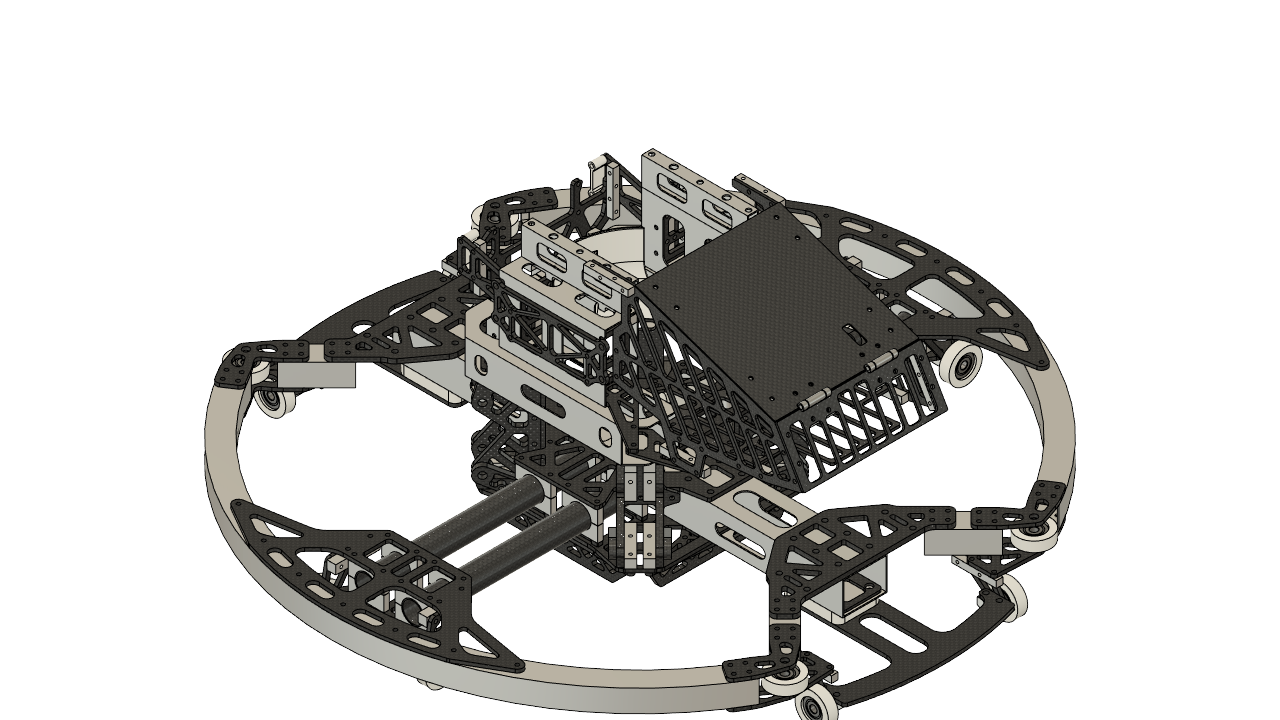
\includegraphics[width=0.45\columnwidth]{figure/设计方案/机械结构设计/步兵弹仓以及基座示意图.png}
    }
    \subfigure[哨兵1代弹仓以及基座示意图\label{fig:哨兵1代弹仓以及基座示意图}]{
        \centering
        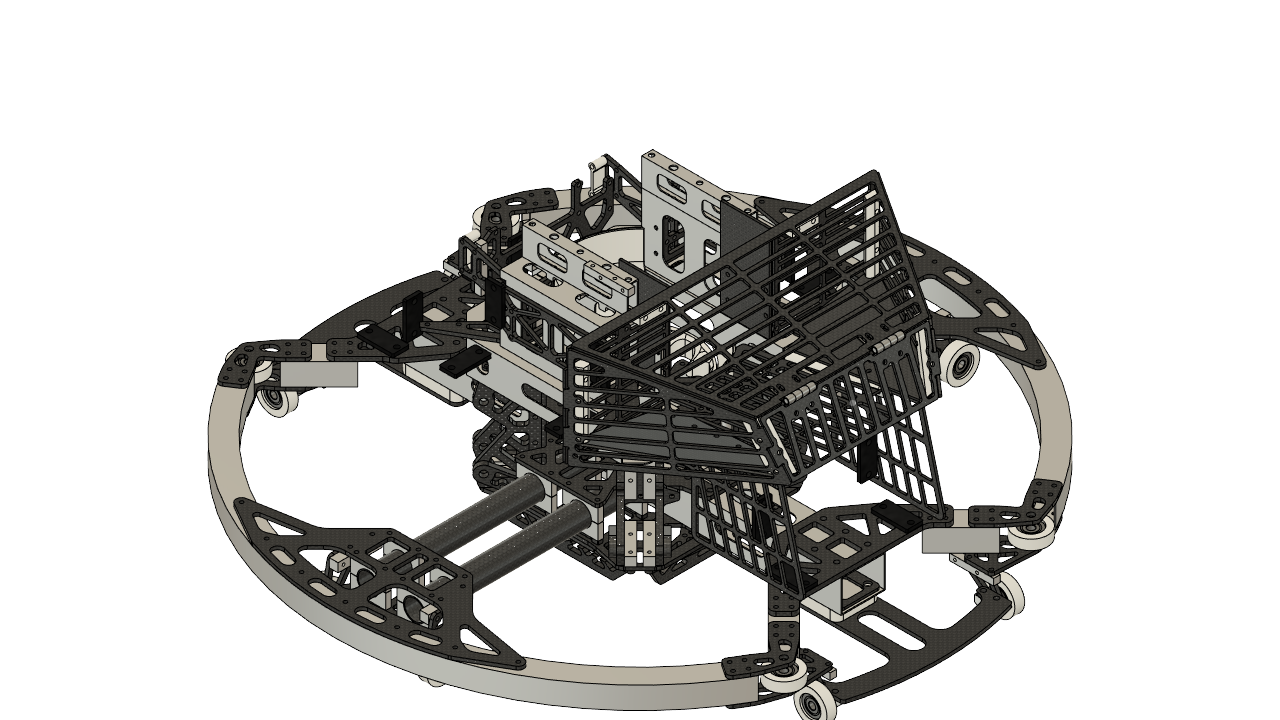
\includegraphics[width=0.45\columnwidth]{figure/设计方案/机械结构设计/哨兵1代弹仓以及基座示意图.png}
    }
    \caption{第一次迭代方案\label{fig:第一次迭代方案}}
\end{figure}

于是我们决定在不改变哨兵轮系结构与悬挂系统的前提下，扩大哨兵车架的尺寸。二代哨兵底盘扩大了云台安装座固定铝管的间距与保护框的大小，使得弹仓可修改的空间更大。扩大基座铝管的间距增大了哨兵的容弹量，同时减少了弹丸对底盘重心的影响。考虑弹丸的随机堆积后，根据公式：
$$N=k*(V_x \div V)$$
其中N为理论装弹量，$V_x$是弹仓容积，V为单颗弹丸体积，k为随机堆积密度，取$60\%$。经过计算，哨兵的基座下方可容纳弹丸465发，经过更改的弹仓可容纳646发，总计可容纳1112发弹丸，可以满足哨兵750发弹丸的需求，如 \figref{fig:第二次迭代方案}所示。云台安装座采用薄壁铝管层叠的方式，在减少质量的同时可以提高强度。

\begin{figure}[hbt!]
    \centering
    \subfigure[哨兵1代弹仓以及基座示意图\label{fig:哨兵1代弹仓以及基座示意图.png} ]{
        \centering
        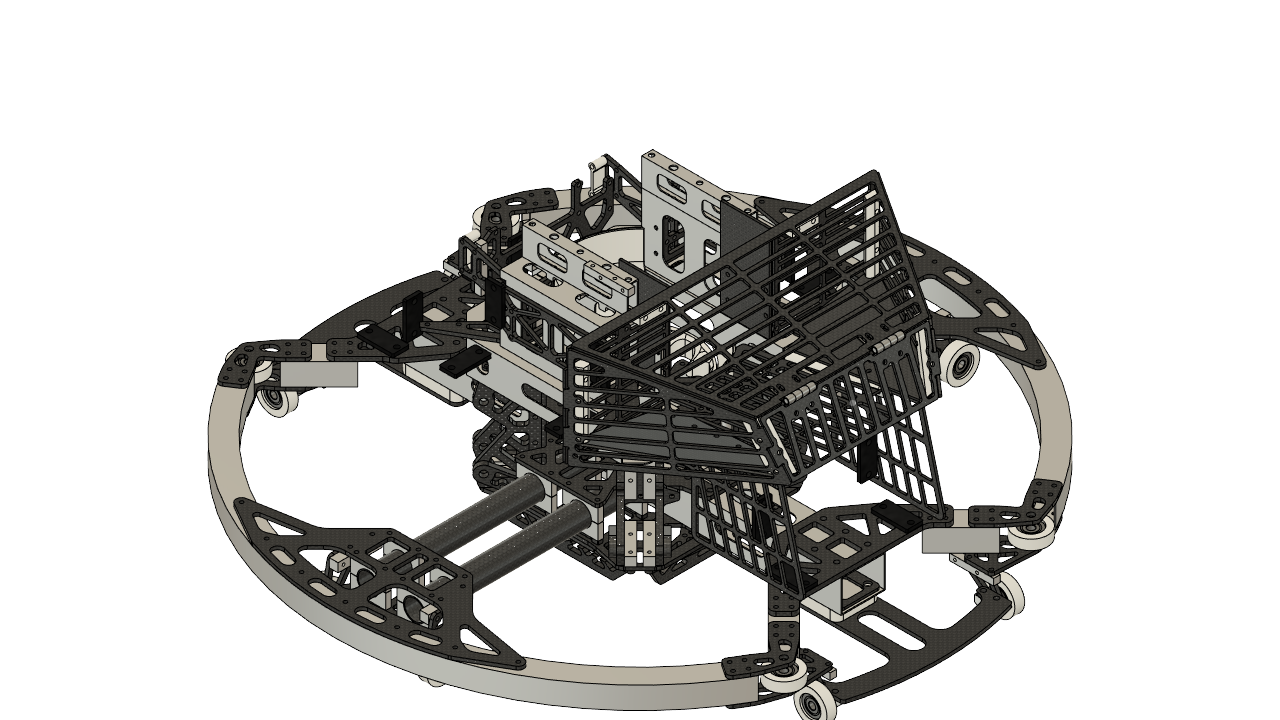
\includegraphics[width=0.45\columnwidth]{figure/设计方案/机械结构设计/哨兵1代弹仓以及基座示意图.png}
    }   
    \subfigure[哨兵2代弹仓以及基座示意图\label{fig:哨兵2代弹仓以及基座示意图}]{
        \centering
        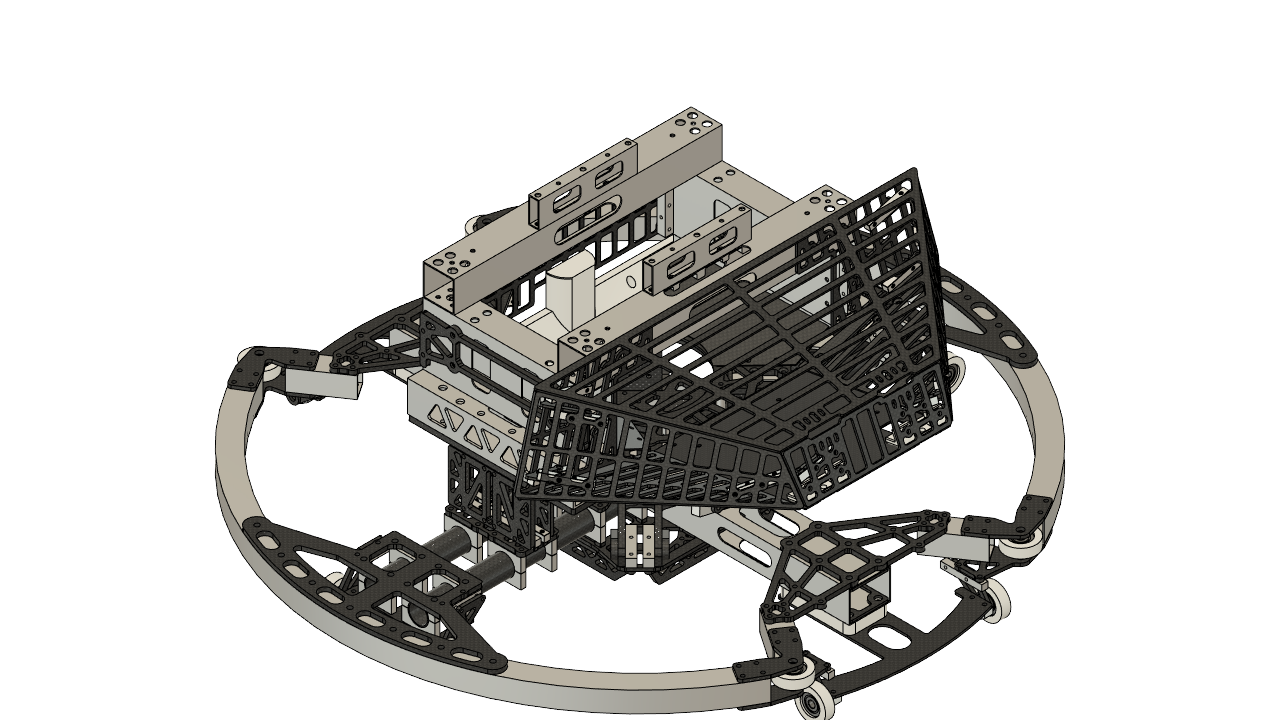
\includegraphics[width=0.45\columnwidth]{figure/设计方案/机械结构设计/哨兵2代弹仓以及基座示意图.png}
    }
    \caption{第二次迭代方案\label{fig:第二次迭代方案}}
\end{figure}

\subsubsection{车架结构}
车架主体采用薄壁粗铝方管，质量轻强度高。如 \figref{fig:拉铆螺母装在铝管内_设计方案}所示我们在铝方管内嵌固定了拉铆螺母的碳板，这样铝管和铝管的连接就无需焊接，同时极大地简化了哨兵底盘的拆装，并且由于碳板直接压在铝管上，碳板可以分散螺丝的拉力，降低铝管撕裂的可能性，但需要定期检查。

\begin{figure}[hbt!]
    \centering
    \subfigure[拉铆螺母固定板\label{fig:拉铆螺母固定板_设计方案} ]{
        \centering
        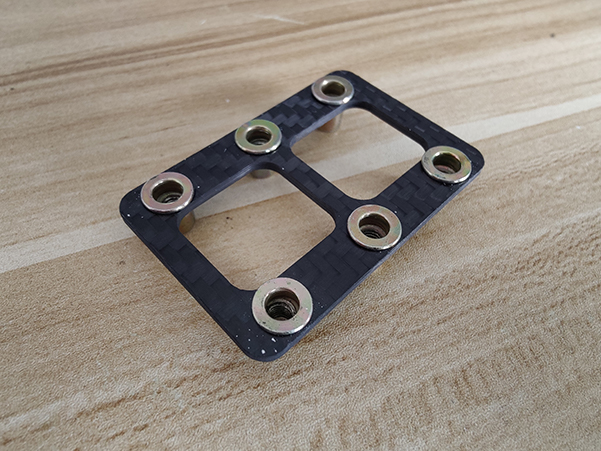
\includegraphics[width=0.4\columnwidth]{figure/设计方案/机械结构设计/拉铆螺母固定板.jpg}
    }
    \subfigure[拉铆螺母装在铝管内\label{fig:拉铆螺母装在铝管内_设计方案}]{
        \centering
        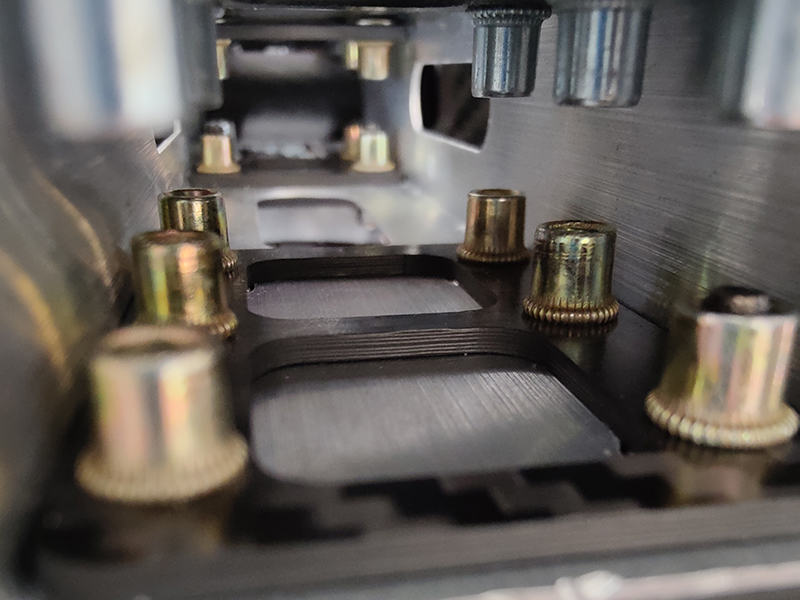
\includegraphics[width=0.4\columnwidth]{figure/设计方案/机械结构设计/拉铆螺母装在铝管内.jpg}
    }
    \caption{铝管连接方式展示\label{fig:铝管连接方式展示_设计方案}}
\end{figure}

如 \figref{fig:chassis1_设计方案}所示车架左右保护框采用碳管与铝方管连接，质量轻强度高且不会因为堆叠碳管而增加车体高度。

结合全向轮布局，我们将保护框设计为圆形，可有效减小因场地因素或对方机器人对哨兵机器人移动和小陀螺的影响，因此保护框采用$\qtyproduct{20 x 20 x 1}{\mm}$的6063铝合金方管弯曲而成，弯曲后将一个带有保护框形状的槽和孔位的2.5D雕刻的玻纤模具扣在方管上打孔并切去多余部分，这样制成的保护框质量轻强度高且成本低。
保护框与车架采用碳板连接，在承受大载荷冲击时共同吸收能量，保护车架。

如 \figref{fig:chassis2_设计方案}所示车架四周安装有落地防卡导轮，防止飞坡姿态不稳定时落地倒栽和脱落下台阶时卡住。底部RFID使用碳板转接，旨在方便拆装而不影响其他零部件，比如需要拆卸裁判系统。RFID四周有碳板保护，防止哨兵在下台阶时损坏RFID或被台阶卡住。

\begin{figure}[hbt!]
    \centering
    \subfigure[车架图\label{fig:chassis1_设计方案} ]{
        \begin{minipage}[t]{0.45\linewidth}
        \centering
        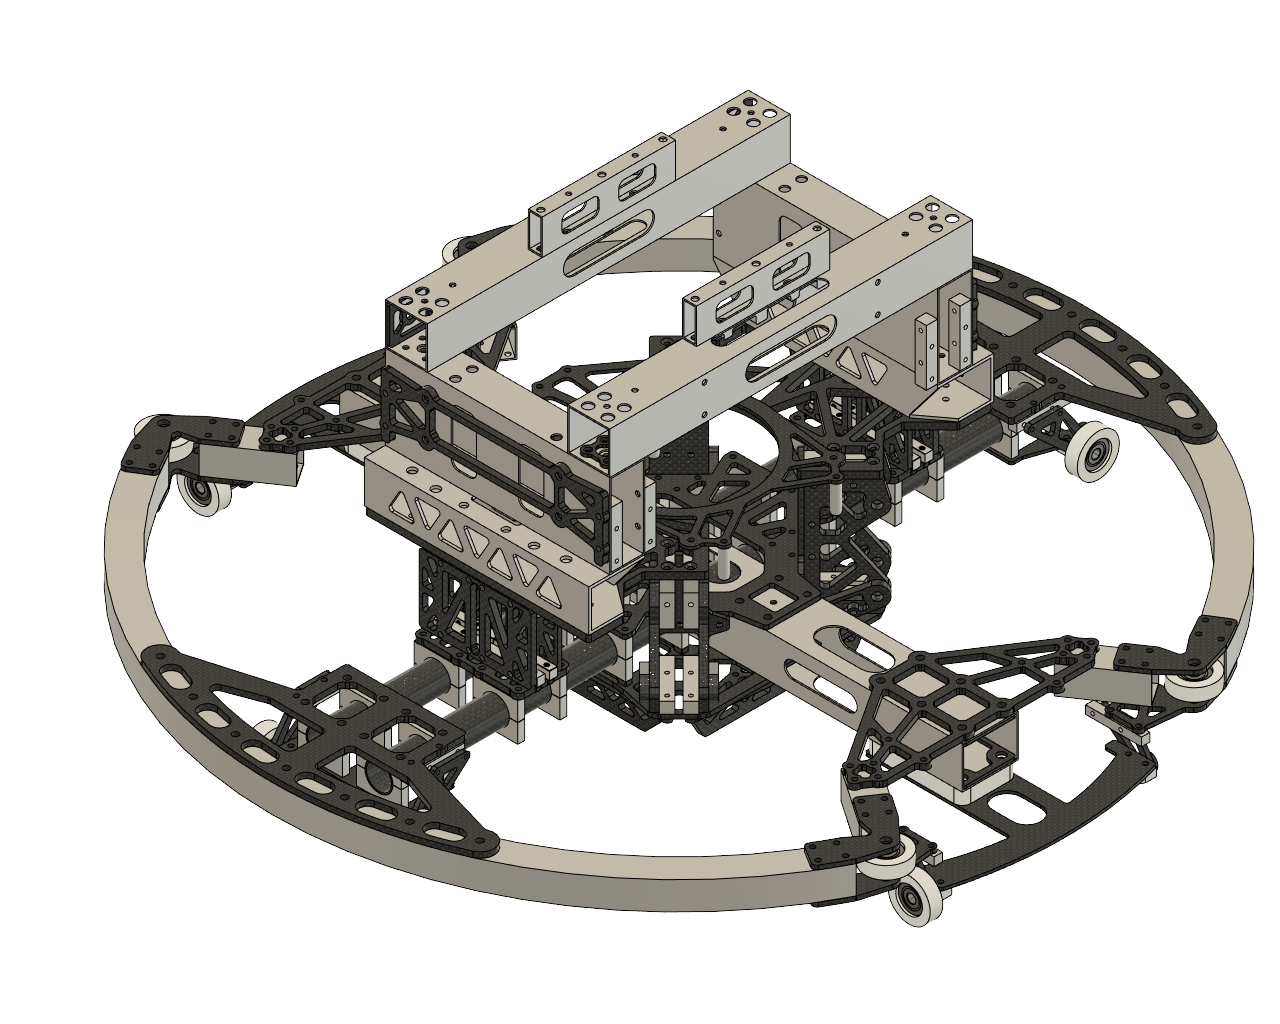
\includegraphics[width=0.7\columnwidth]{figure/设计方案/机械结构设计/车架.png}
        \end{minipage}
    }
    \subfigure[落地防卡导轮\label{fig:chassis2_设计方案}]{
        \begin{minipage}[t]{0.45\linewidth}
        \centering
        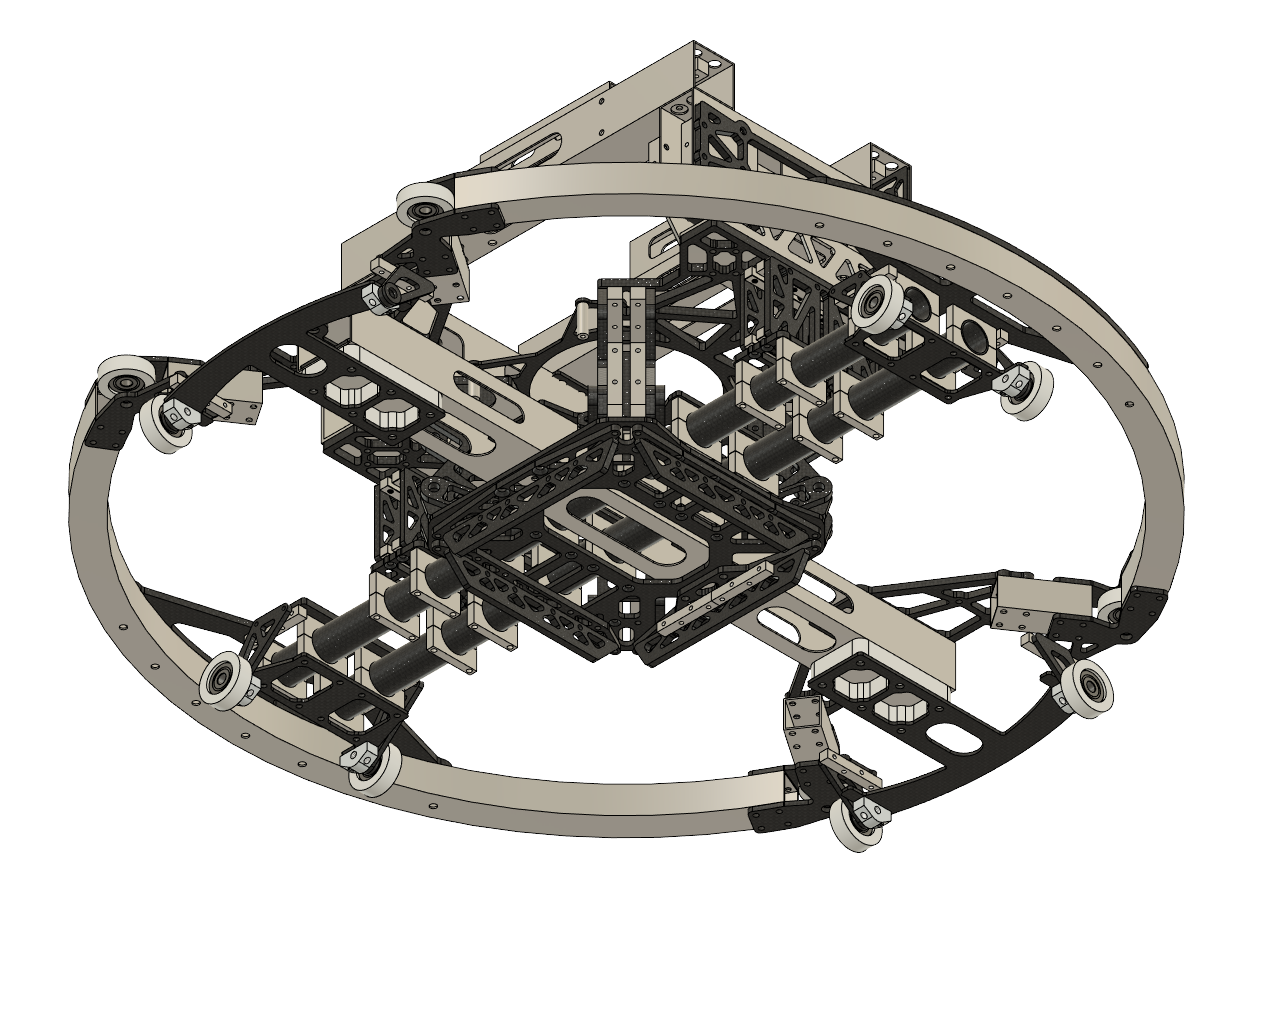
\includegraphics[width=0.7\columnwidth]{figure/设计方案/机械结构设计/落地防卡导轮.png}
        \end{minipage}
    }
    \caption{车架展示\label{fig:chassis3_设计方案}}
\end{figure}

\subsubsection{轮系结构}

为了简化结构和减重，在轮系中我们采用了 如\figref{fig:轮毂电机及其配套的全向轮_设计方案}所示自制的减速箱轮毂电机。

\begin{figure}[hbt!]
    \centering
        \subfigure[轮毂电机质量\label{fig:轮毂电机质量} ]{
        \centering
        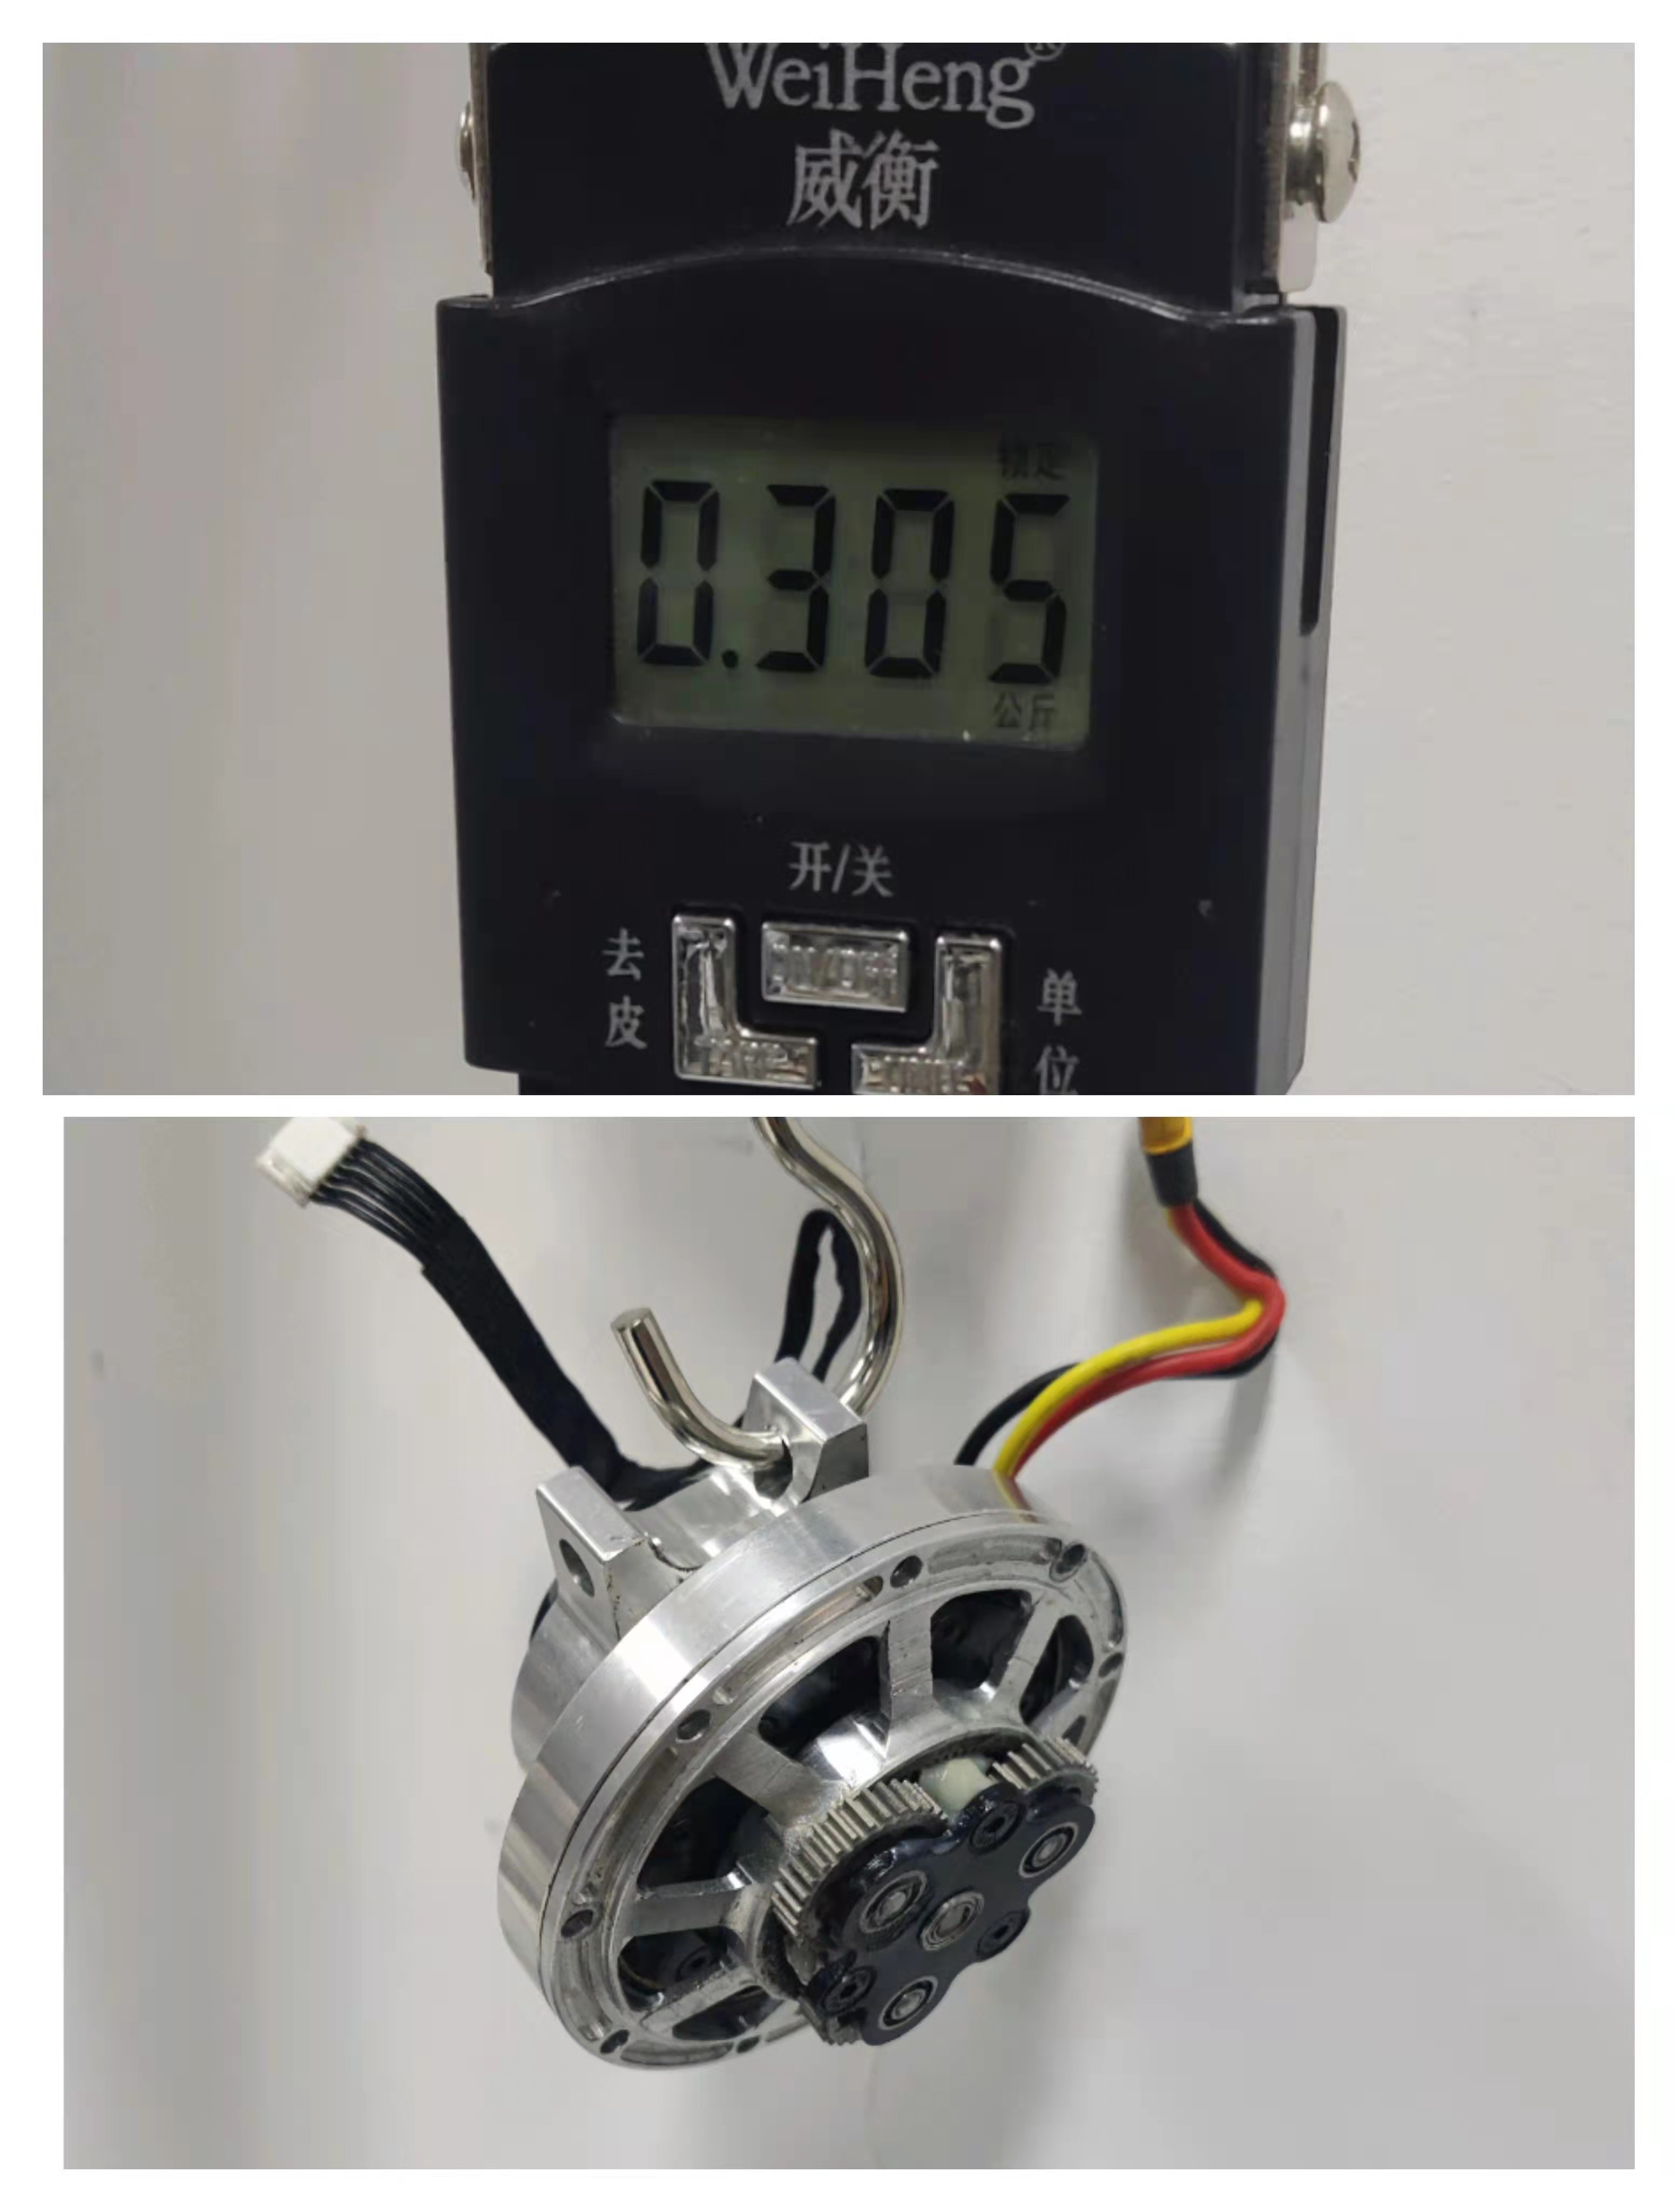
\includegraphics[width=0.15\columnwidth]{figure/设计方案/机械结构设计/轮毂电机质量.jpg}
    }
    \subfigure[轮毂电机图\label{fig:轮毂电机图_设计方案} ]{
        \centering
        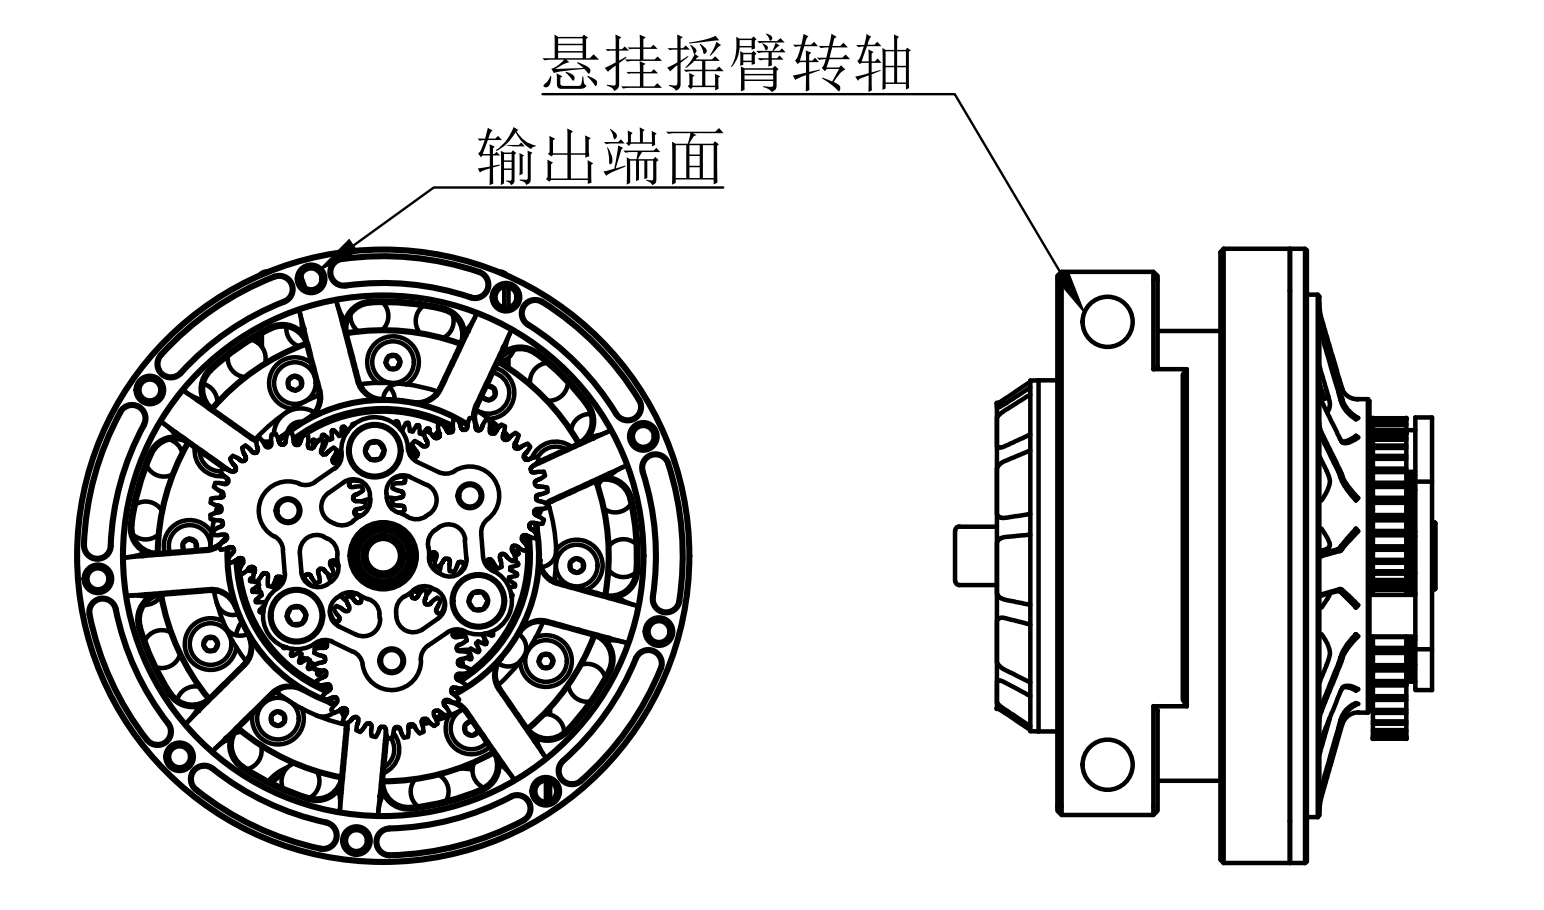
\includegraphics[width=0.35\columnwidth]{figure/设计方案/机械结构设计/轮毂电机图.png}
    }
    \subfigure[6寸全向轮轮毂电机爆炸图\label{fig:6寸全向轮轮毂电机爆炸图_设计方案}]{
        \centering
        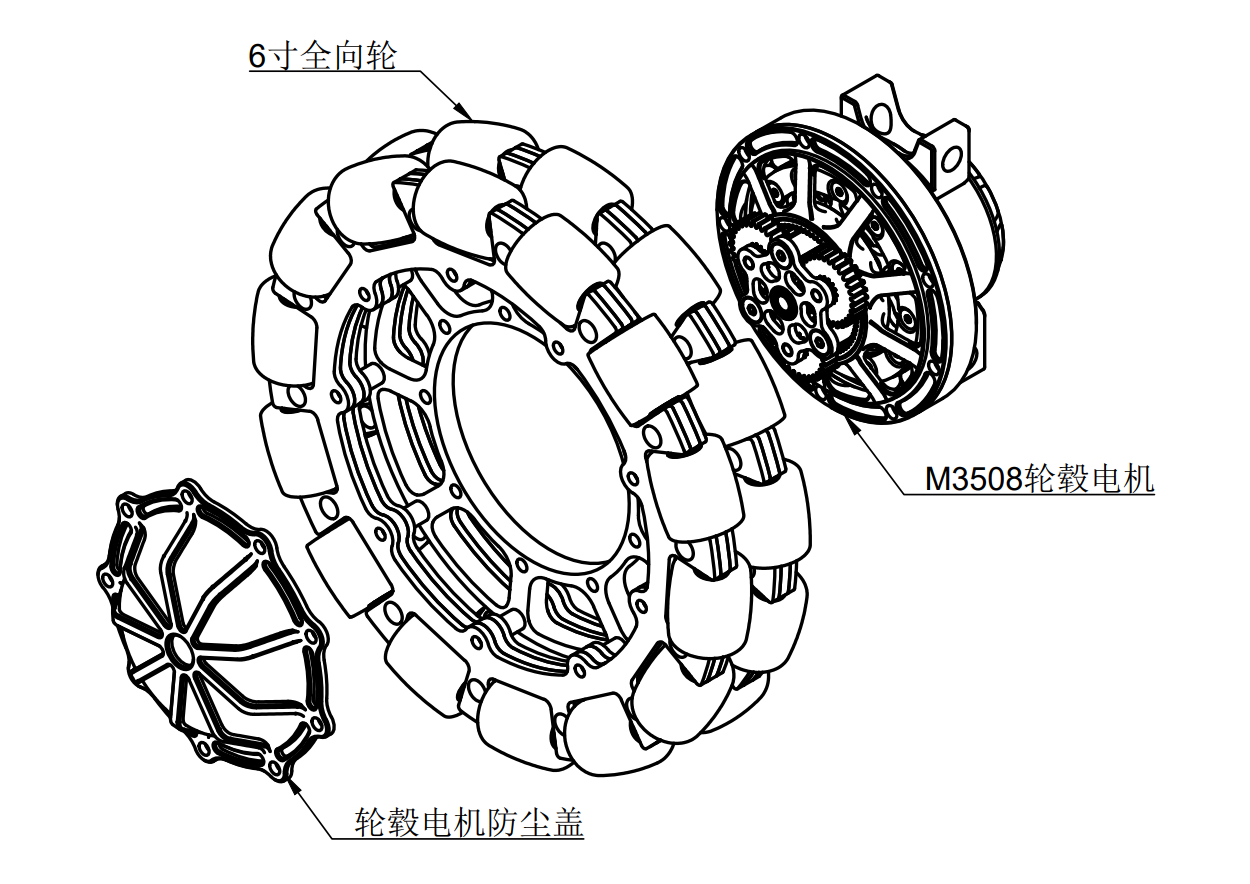
\includegraphics[width=0.35\columnwidth]{figure/设计方案/机械结构设计/6寸全向轮轮毂电机爆炸图.png}
    }
    \caption{轮毂电机及其配套的全向轮\label{fig:轮毂电机及其配套的全向轮_设计方案}}
\end{figure}

该减速器可自由设计减速比（1:11-1:21）同时如 \figref  {fig:两种轮毂电机固定方式_设计方案}所示输入端可根据需求改变固定方式，例如采用端面固定或四连杆摇臂。轮毂电机采用一个大号四点接触轴承作为输出端轴承，提高了该电机的抗冲击能力，同时简化了轴系，降低了全向轮的拆装的难度。

\begin{figure}[hbt!]
    \centering
    \subfigure[轮毂电机四连杆摇臂固定\label{fig:轮毂电机四连杆摇臂固定_设计方案} ]{
        \centering
        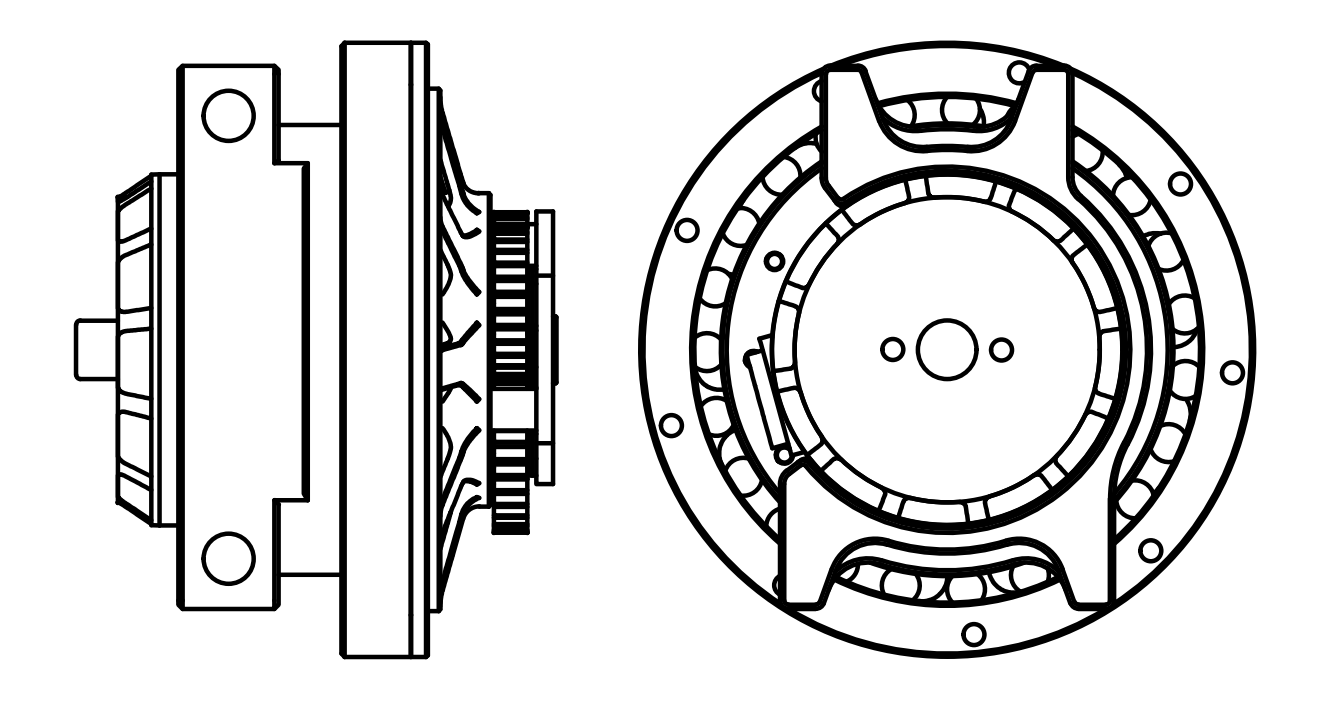
\includegraphics[width=0.40\columnwidth]{figure/设计方案/机械结构设计/轮毂电机四连杆摇臂固定.png}
    }
    \subfigure[轮毂电机端面固定\label{fig:轮毂电机端面固定_设计方案}]{
        \centering
        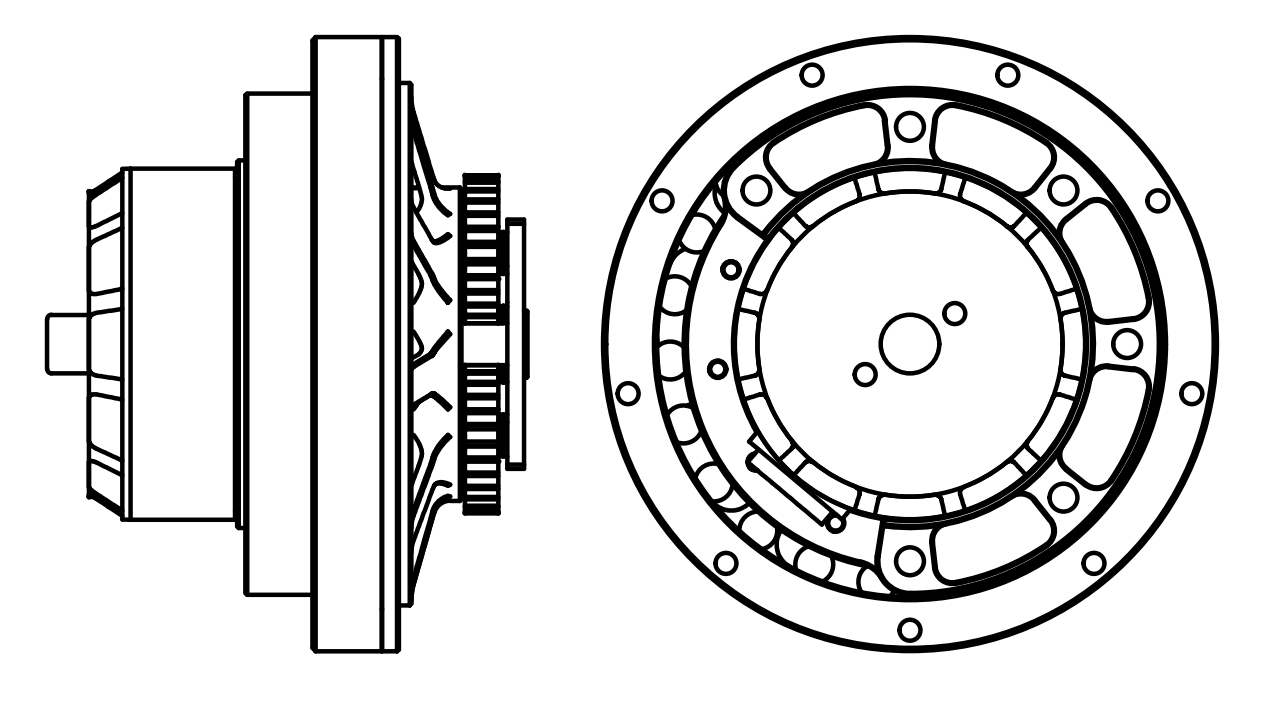
\includegraphics[width=0.40\columnwidth]{figure/设计方案/机械结构设计/轮毂电机端面固定.png}
    }
    \caption{两种轮毂电机固定方式\label{fig:两种轮毂电机固定方式_设计方案}}
\end{figure}

该电机在采用端面固定的时候仅重约$\qty{270}{\g}$，并且由于减速器采用端面输出，不用像原装M3508一样添加联轴器即可固定轮子。如\figref {fig:悬挂系统质量对比_设计方案}所示，更换轮毂电机后减重效果显著，整车可减重$\qty{1.4}{\kilogram}$。

\begin{figure}[hbt!]
    \centering
    \subfigure[原装M3508悬挂系统系统质量\label{fig:原装M3508悬挂系统系统质量_设计方案} ]{
        \centering
        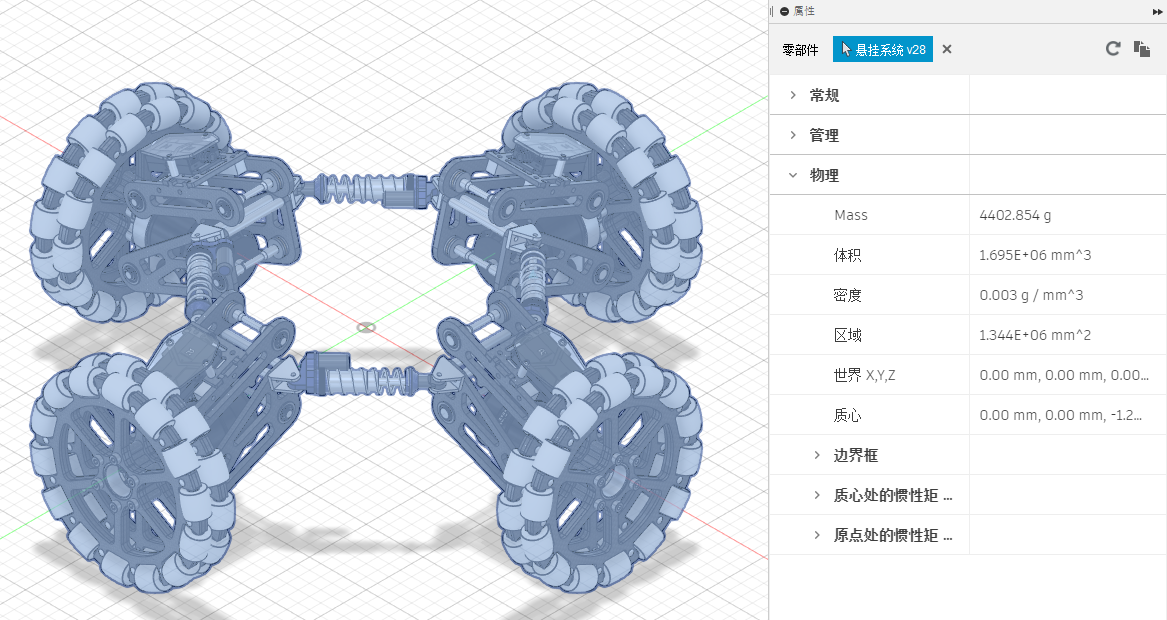
\includegraphics[width=0.40\columnwidth]{figure/设计方案/机械结构设计/原装M3508悬挂系统系统质量.png}
    }
    \subfigure[轮毂电机悬挂系统系统质量\label{fig:轮毂电机悬挂系统系统质量_设计方案}]{
        \centering
        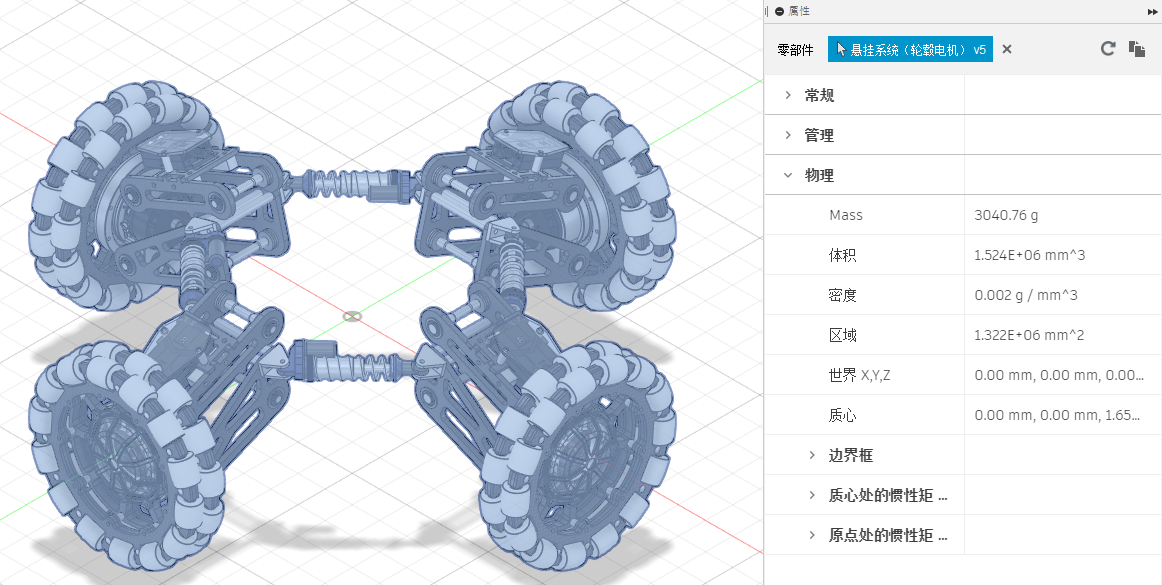
\includegraphics[width=0.40\columnwidth]{figure/设计方案/机械结构设计/轮毂电机悬挂系统系统质量.png}
    }
    \caption{悬挂系统质量对比\label{fig:悬挂系统质量对比_设计方案}}
\end{figure}

\subsubsection{自适应悬挂结构}

如 \figref{fig:悬挂系统展示_设计方案}我们采用了与哈工大深圳开源步兵相似的环式自适应平行四边形悬挂，四个避震器水平放置介于两轮组之间。保证轮组抓地、结构简单、可以空出中心云台位置。但根据底盘布局将避震器的安装位置下移，提高了底盘的空间利用率。通过设计自适应行程，确保底盘在小陀螺上坡时不会有轮子悬空。
同时，为提高小陀螺旋转速度，我们尽可能的减小了全向轮对边的轮距。

\begin{figure}[hbt!]
    \centering
    \subfigure[悬挂系统图]{
        \begin{minipage}[t]{0.45\linewidth}
        \centering
        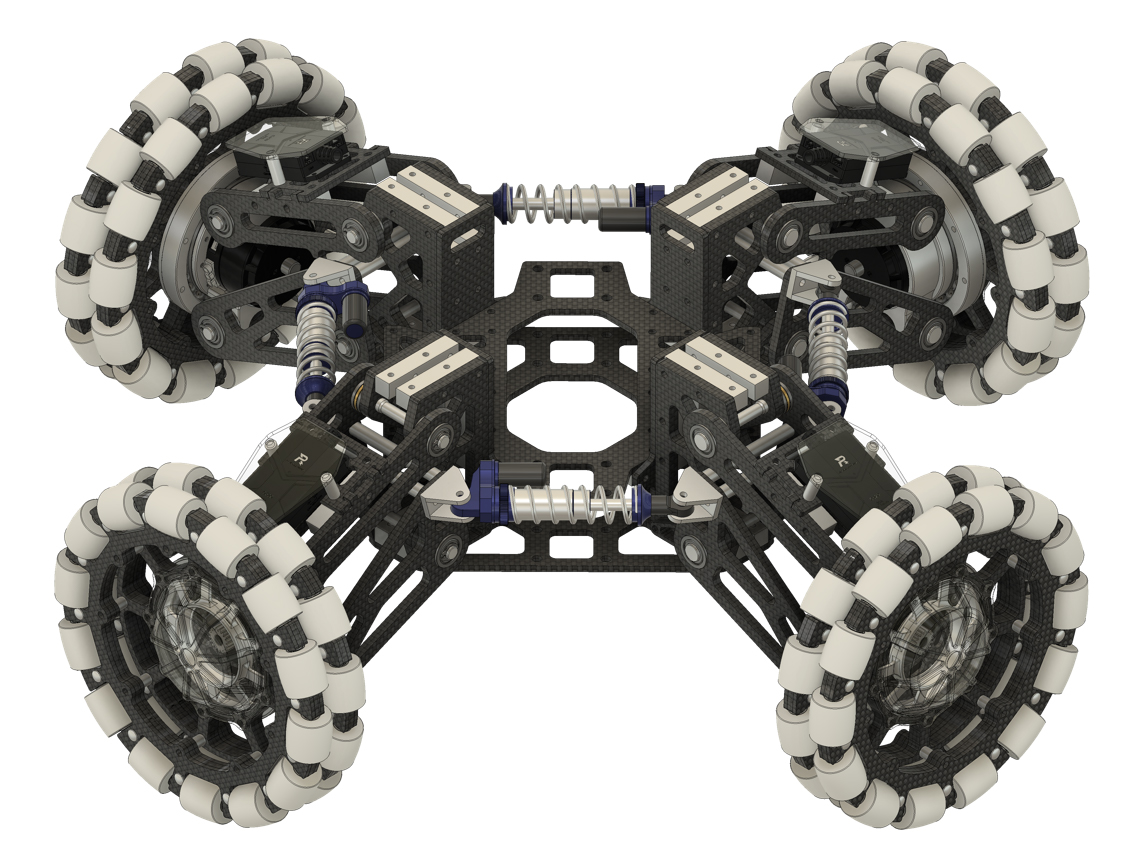
\includegraphics[width=0.7\columnwidth]{figure/设计方案/机械结构设计/悬挂系统图.jpg}
        \end{minipage}
    }
    \subfigure[轮距图]{
        \begin{minipage}[t]{0.45\linewidth}
        \centering
        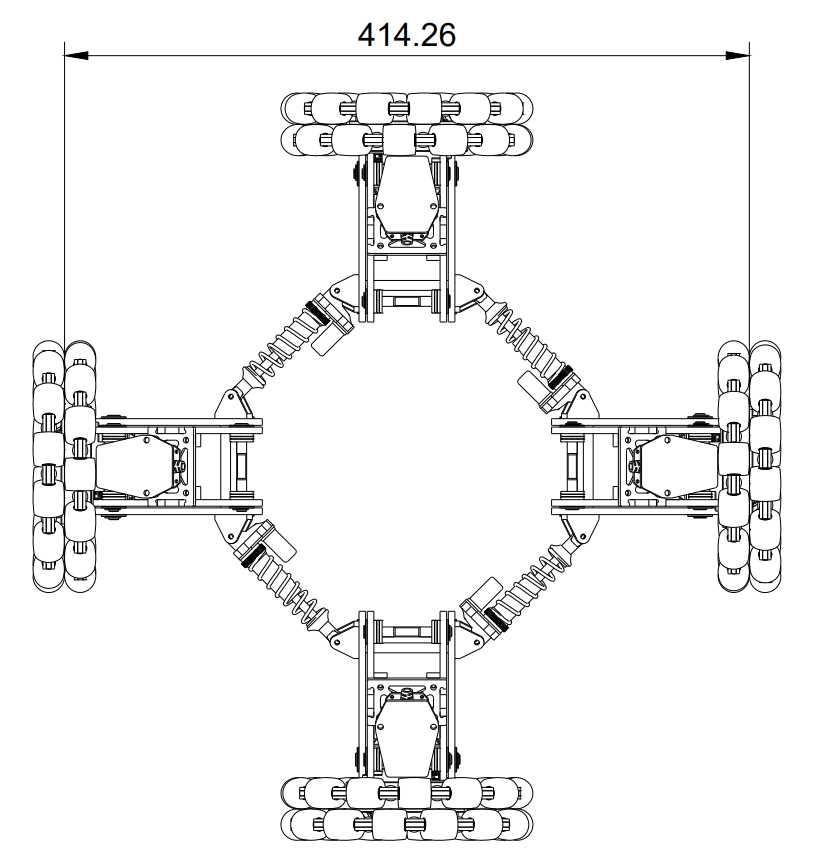
\includegraphics[width=0.7\columnwidth]{figure/设计方案/机械结构设计/轮距图.png}
        \end{minipage}
    }
    \caption{悬挂系统展示}
    \label{fig:悬挂系统展示_设计方案}
\end{figure}


\subsubsection{云台设计}

\paragraph{云台架结构}
如\figref {fig:Yaw轴转轴展示_设计方案}
所展示，Yaw轴轴承为了稳定性采用RA5008交叉滚子轴承，间隙极小,抗冲击性能好，可以多次承受飞坡失败时的冲击而不失效。

\begin{figure}[hbt!]
    \centering
    \subfigure[Yaw轴转轴\label{fig:Yaw轴转轴_设计方案} ]{
        \begin{minipage}[t]{0.45\linewidth}
        \centering
        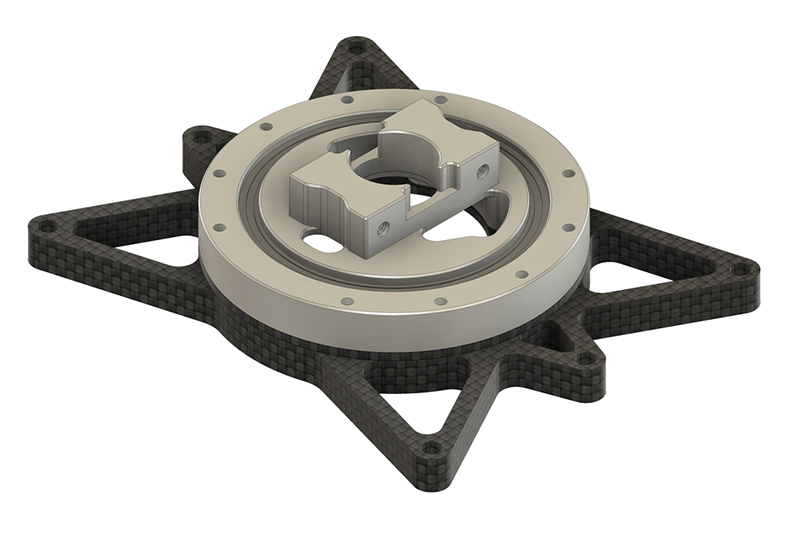
\includegraphics[width=0.7\columnwidth]{figure/设计方案/机械结构设计/yaw轴转轴.jpg}
        \end{minipage}
    }
    \subfigure[Yaw轴转轴爆炸图\label{fig:Yaw轴转轴爆炸图_设计方案}]{
        \begin{minipage}[t]{0.45\linewidth}
        \centering
        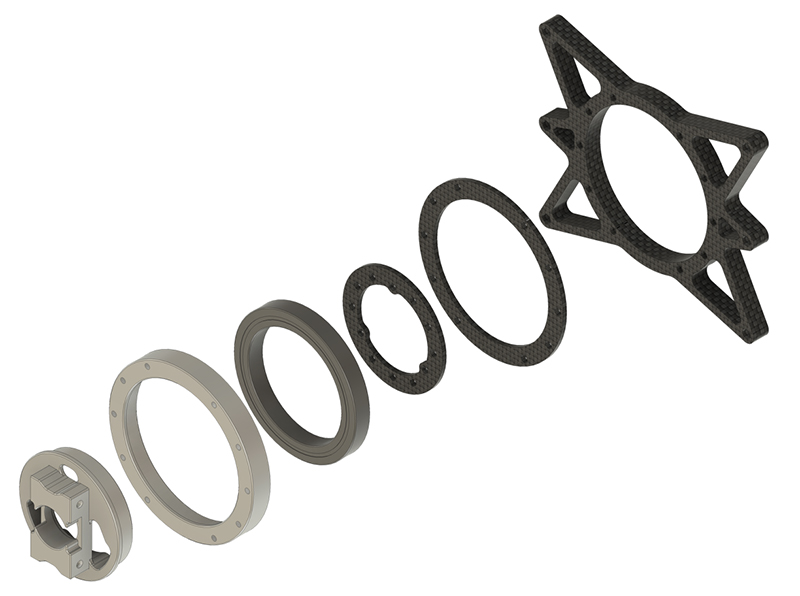
\includegraphics[width=0.7\columnwidth]{figure/设计方案/机械结构设计/yaw轴转轴爆炸图.jpg}
        \end{minipage}
    }
    \caption{Yaw轴转轴展示\label{fig:Yaw轴转轴展示_设计方案}}
\end{figure}

如 \figref {fig:云台支架展示_设计方案}
所展示，为了减小Yaw轴转动惯量，云台架结构沿Yaw轴分布。为配合两侧装甲板高度并满足规则限高，我们将云台Pitch轴转轴到Yaw轴轴承的高度降低至$\qty{90}{\mm}$，依然满足云台$\ang{30}$俯角，同时减短了弹链长度，并可以满足哨兵、步兵和无人机的使用需求。云台架主体采用两块$\qty{5}{\mm}$碳板做支撑，质量轻强度高。为减小Pitch轴惯量，我们没有选择将电机放置Pitch轴上做配平，而是将Pitch轴的M3508P11（详见\ref{M3508P11}）固定在云台支架通过连杆驱动云台俯仰。

\begin{figure}[hbt!]
    \centering
    \subfigure[云台支架斜二测 隐藏minipc和雷达\label{fig:云台支架斜二测 隐藏minipc和雷达_设计方案} ]{
        \begin{minipage}[t]{0.45\linewidth}
        \centering
        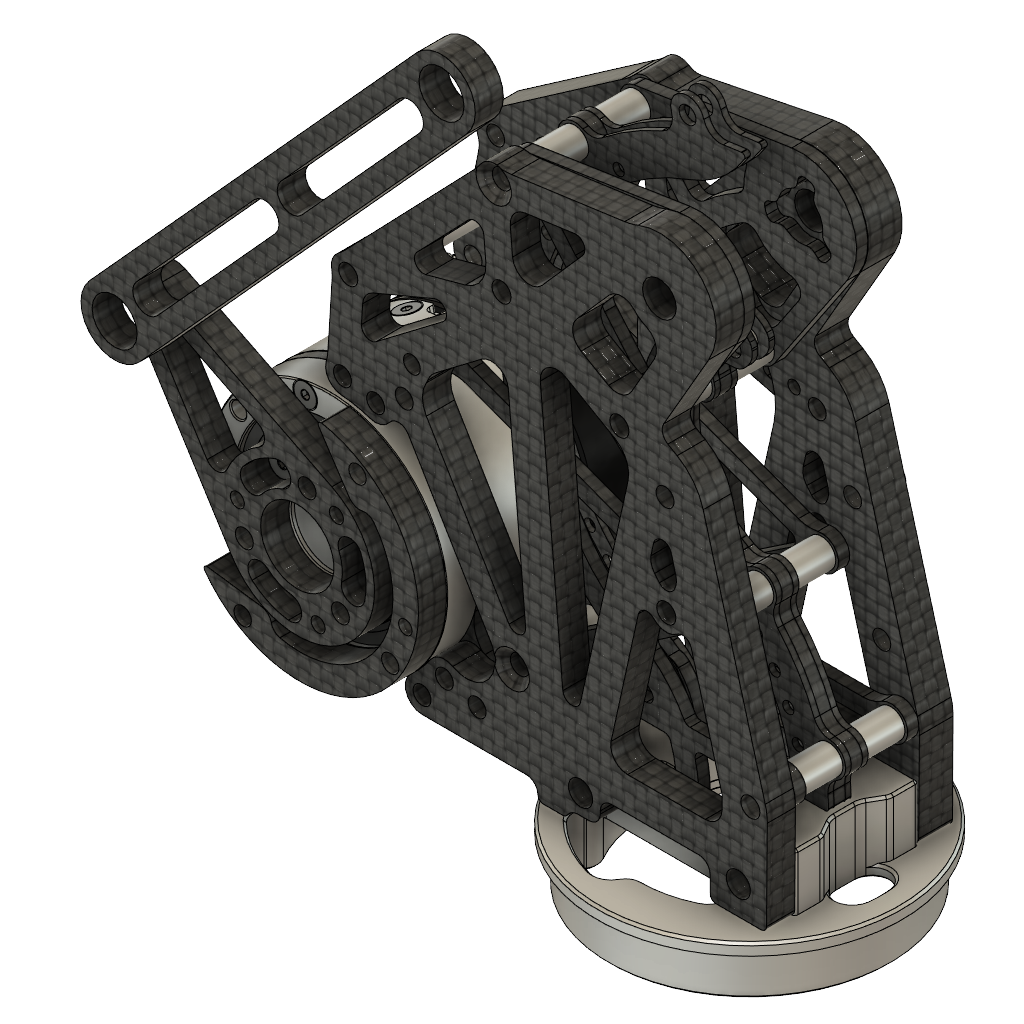
\includegraphics[width=0.7\columnwidth]{figure/设计方案/机械结构设计/云台支架斜二测 隐藏minipc和雷达.png}
        \end{minipage}
    }
    \subfigure[云台支架侧视图 隐藏minipc和雷达\label{fig:云台支架侧视图 隐藏minipc和雷达_设计方案}]{
        \begin{minipage}[t]{0.45\linewidth}
        \centering
        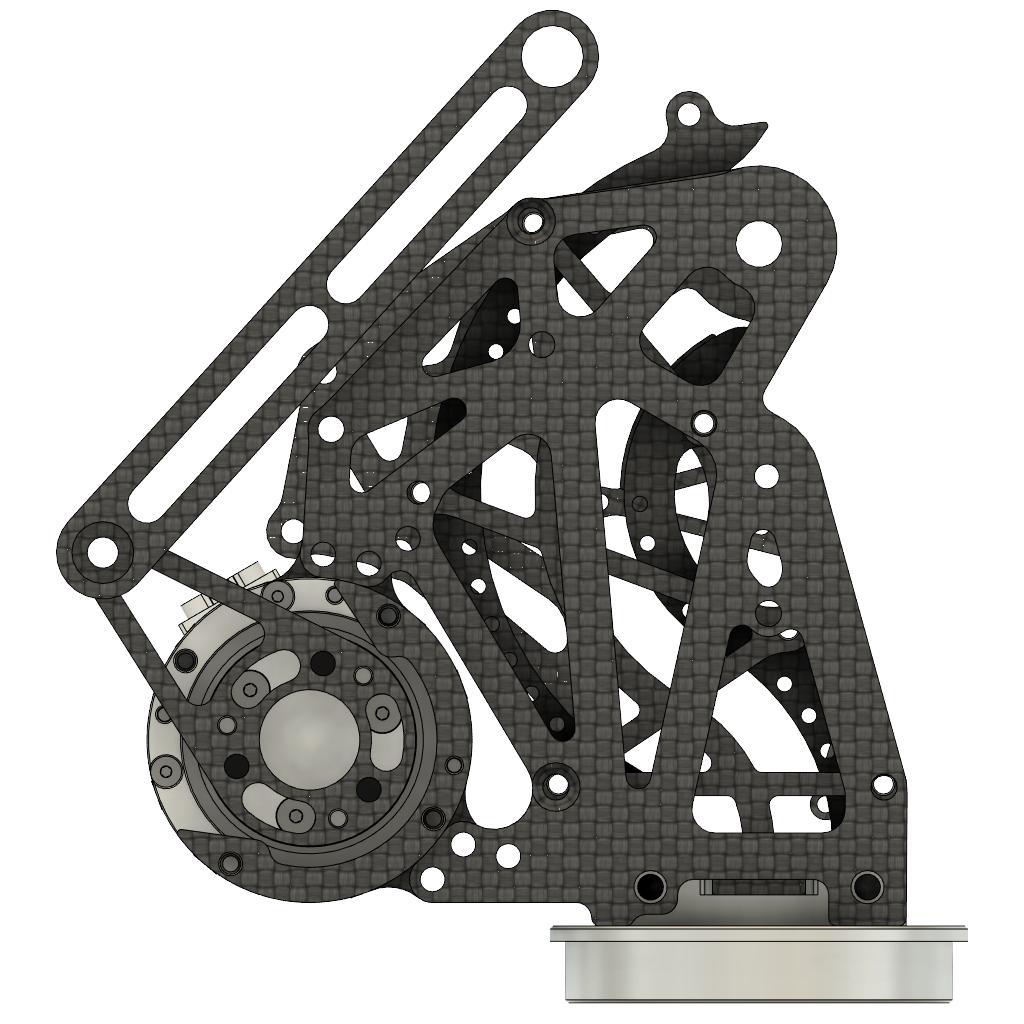
\includegraphics[width=0.7\columnwidth]{figure/设计方案/机械结构设计/云台支架侧视图 隐藏minipc和雷达.png}
        \end{minipage}
    }
    \caption{云台支架展示\label{fig:云台支架展示_设计方案}}
\end{figure}

如 \figref {fig:Mini PC和UWB安装图_设计方案}
所展示，由于我们采用中置的弹链，Mini PC挂在云台架侧面。为保护Mini PC，我们在Mini PC外添加了一个碳纤维板构成的保护壳，并留出空间用来理线和放置usb2can等模块。

由于定位模块上方 $\ang{145}$内不得被导体遮挡，我们将UWB架高位于除灯条以外的所有结构之上，采用两根$\qty{8}{\mm}$的薄壁碳管配合管夹和$\qty{2}{\mm}$及$\qty{4}{\mm}$的板件组成UWB支架。

\begin{figure}[hbt!]
    \centering
    \subfigure[云台支架Mini PC保护\label{fig:云台支架Mini PC保护_设计方案} ]{
        \begin{minipage}[t]{0.45\linewidth}
        \centering
        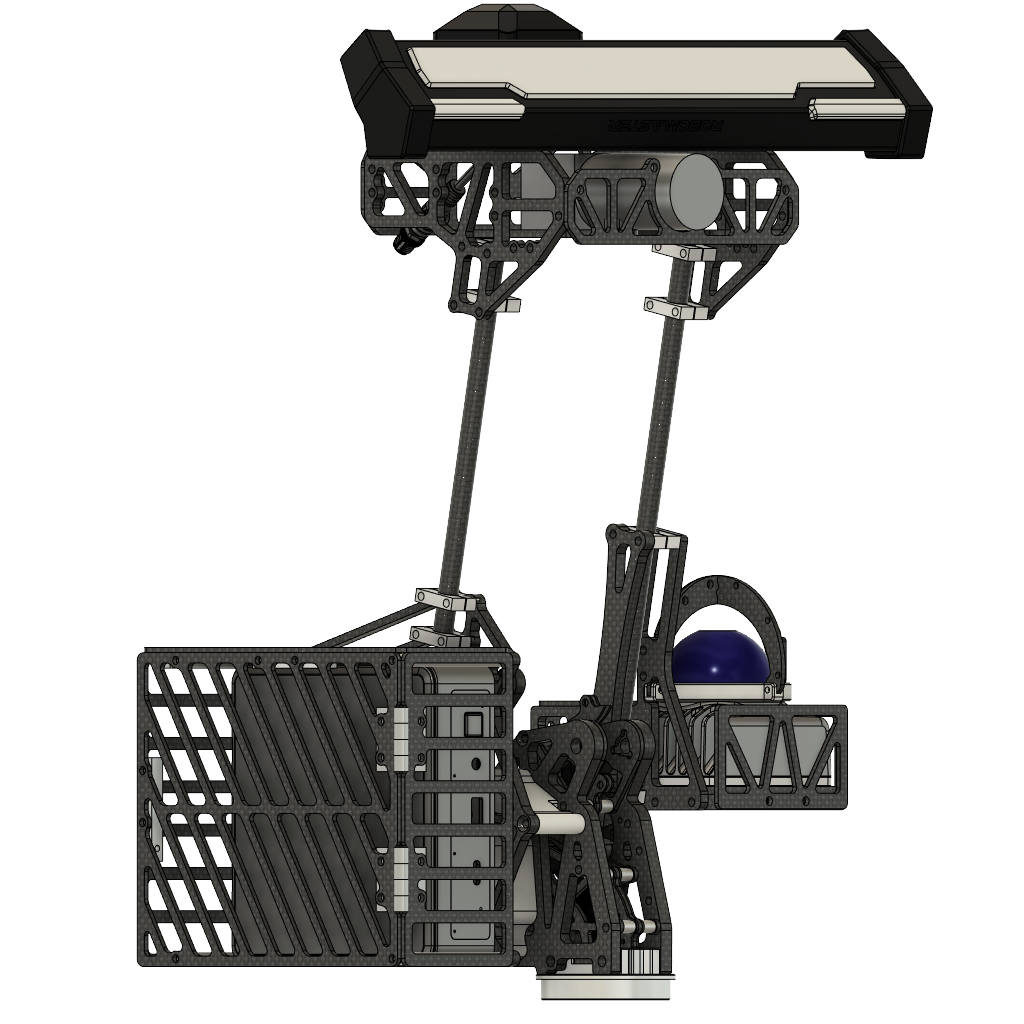
\includegraphics[width=0.7\columnwidth]{figure/设计方案/机械结构设计/云台支架Mini PC保护.png}
        \end{minipage}
    }
    \subfigure[云台支架UWB固定\label{fig:云台支架UWB固定_设计方案}]{
        \begin{minipage}[t]{0.45\linewidth}
        \centering
        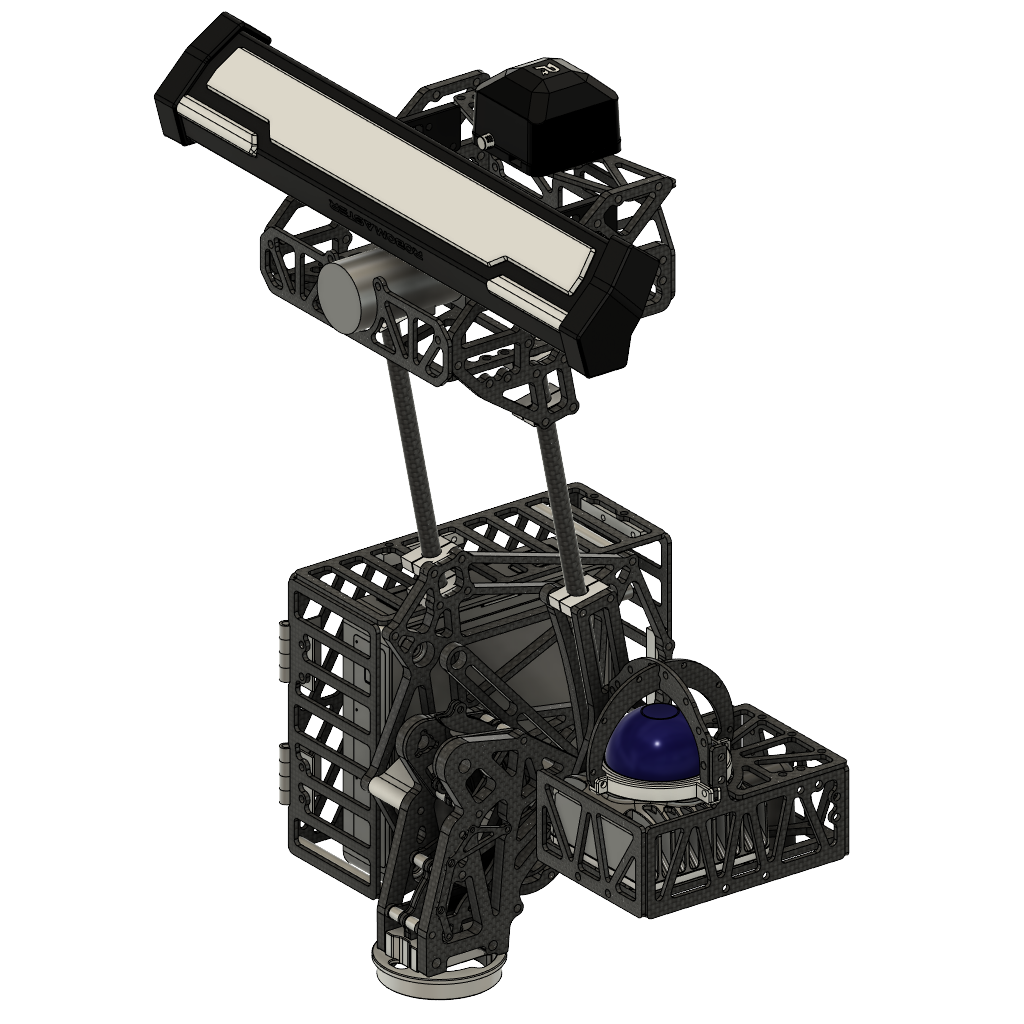
\includegraphics[width=0.7\columnwidth]{figure/设计方案/机械结构设计/云台支架UWB固定.png}
        \end{minipage}
    }
    \caption{Mini PC和UWB安装图\label{fig:Mini PC和UWB安装图_设计方案}}
\end{figure}

\paragraph{自制GM6020一体式滑环}

如\figref{fig:GM6020外套滑环展示_设计方案}所展示，在进行哨兵机器人设计时我们沿用了2022赛季步兵机器人这种将滑环套在电机外部的方案。该方案GM6020可以直驱云台，提高了控制带宽；滑环转子与电机转子固定，与电机共用轴承，降低了Yaw轴的转动阻力。同时我们可以根据不同线路对电流的要求设计滑环电刷导线数量和铜环宽度，降低了滑环的高度和重量。由于该方案电机直驱云台，整个模块的固定仅需7根螺丝，简化了云台的拆装。

\begin{figure}[hbt!]
    \centering
    \subfigure[GM6020外套滑环剖面图\label{fig:GM6020外套滑环剖面图_设计方案} ]{
        \centering
        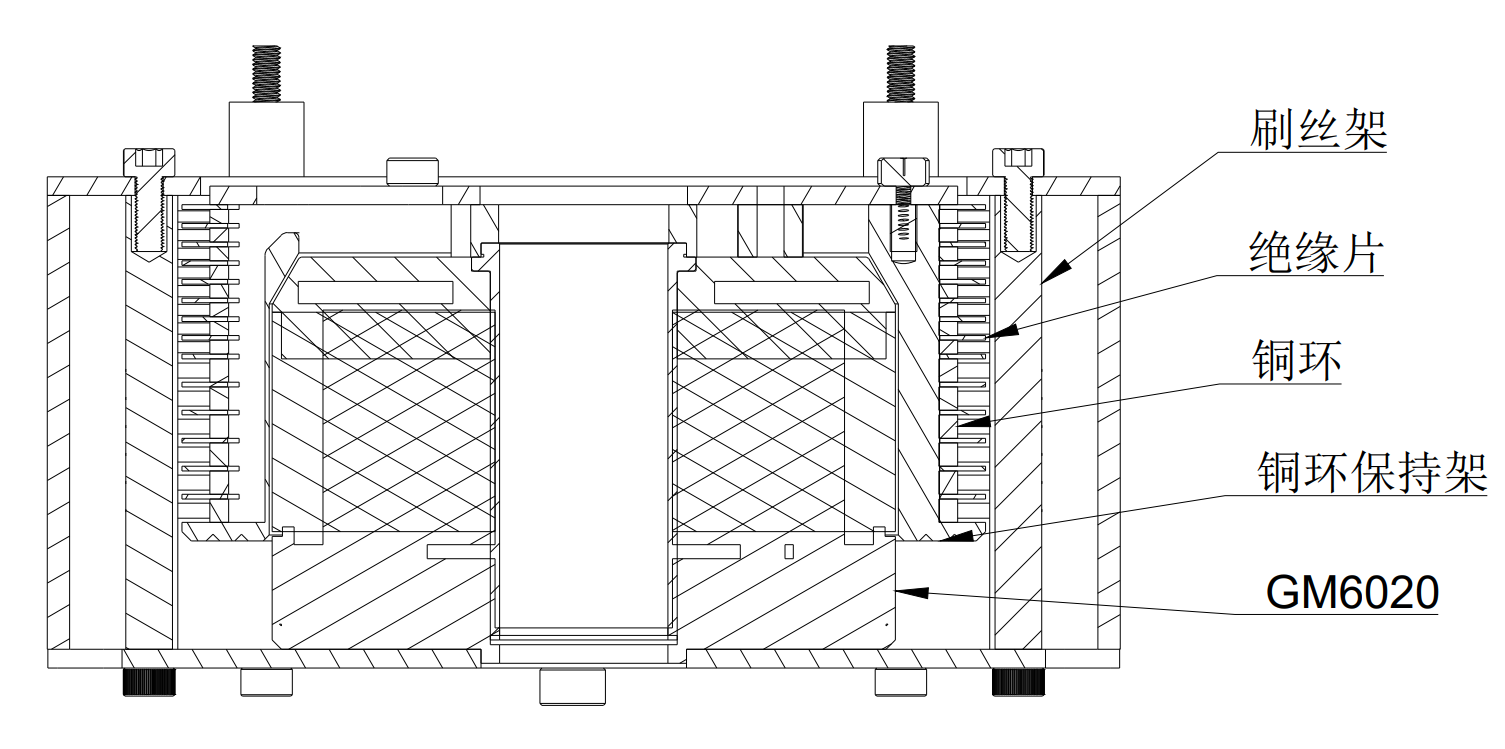
\includegraphics[width=0.45\columnwidth]{figure/设计方案/机械结构设计/GM6020外套滑环剖面图.png}
    }
    \subfigure[GM6020外套滑环实物图\label{fig:GM6020外套滑环实物图_设计方案}]{
        \centering
        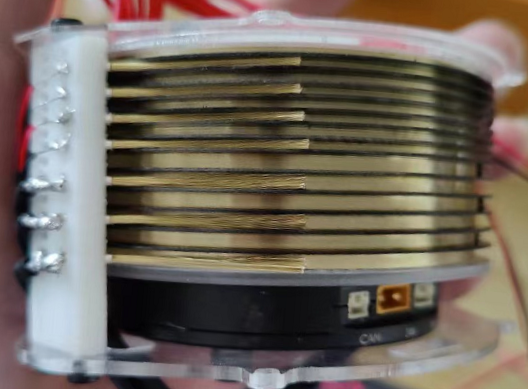
\includegraphics[width=0.25\columnwidth]{figure/设计方案/机械结构设计/GM6020外套滑环实物图.png}
    }
    \caption{GM6020外套滑环展示\label{fig:GM6020外套滑环展示_设计方案}}
\end{figure}

但是在实际使用GM6020外套滑环的过程中，我们发现GM6020外套滑环会出现信号传输不通、使用寿命不够长的问题。在多方咨询和各种尝试后，我们发现原本刷丝和铜环的接触角度不足以保证稳定的信号传输，因此我们增大了刷丝和铜环的接触角度。经测试后发现加大后的接触角度已经可以至少在150个小时工作时间内保证信号可以稳定传输。同时，我们将铜环更换为更耐磨的不锈钢环。

目前经历过升级后的GM6020外套新滑环解决了信号传输不稳定和使用寿命不够长的问题，已经可以满足我们对滑环的使用需求，如\figref{fig:GM6020外套新滑环展示_设计方案}所展示。

\begin{figure}[hbt!]
    \centering
    \subfigure[GM6020外套新滑环剖面图\label{fig:GM6020外套新滑环剖面图_设计方案} ]{
        \centering
        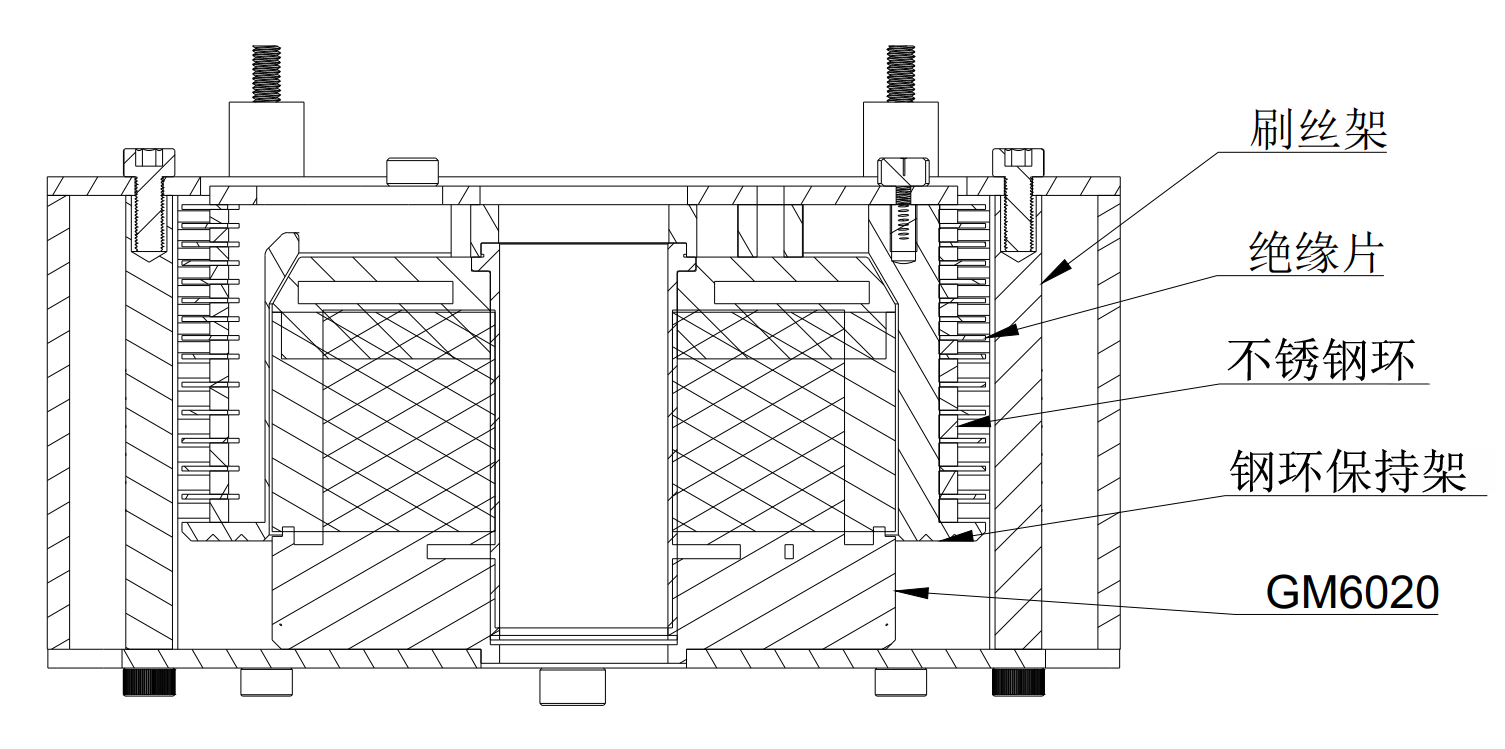
\includegraphics[width=0.45\columnwidth]{figure/设计方案/机械结构设计/GM6020外套新滑环剖面图.png}
    }
    \subfigure[GM6020外套新滑环实物图\label{fig:GM6020外套新滑环实物图_设计方案}]{
        \centering
        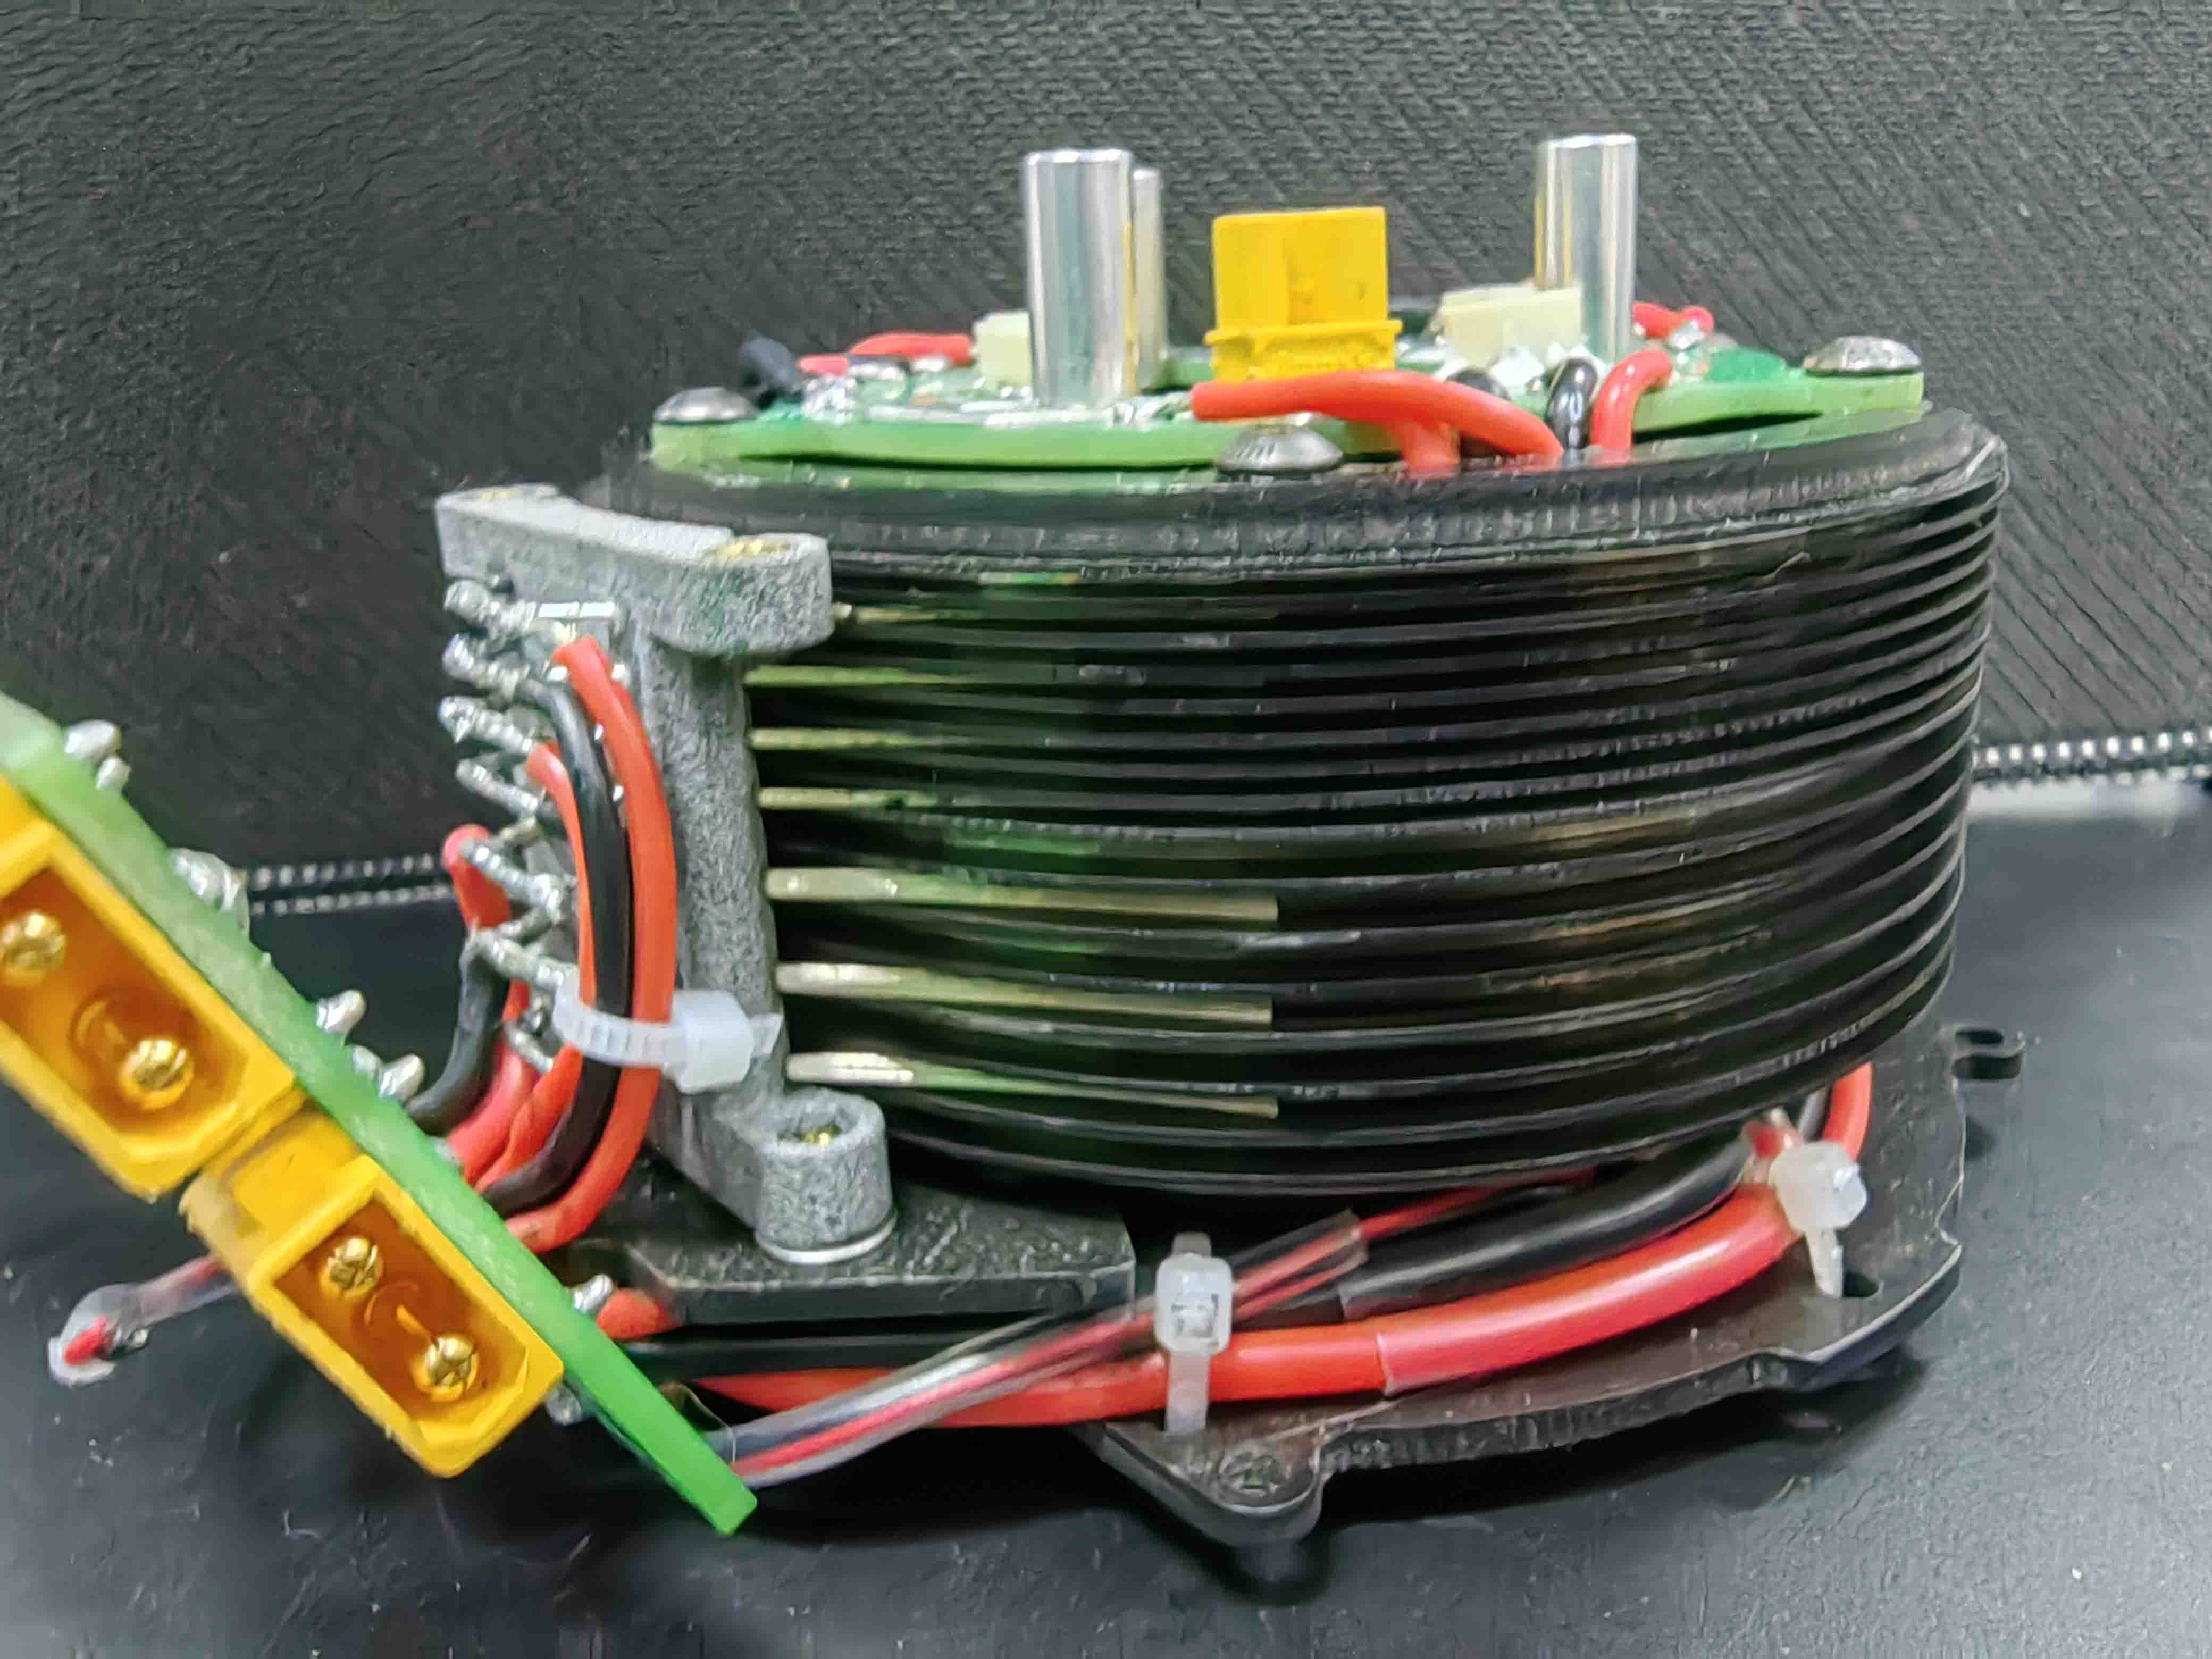
\includegraphics[width=0.25\columnwidth]{figure/设计方案/机械结构设计/GM6020外套新滑环实物图.jpg}
    }
    \caption{GM6020外套新滑环展示\label{fig:GM6020外套新滑环展示_设计方案}}
\end{figure}

然而为了追求更稳定的Yaw轴云台响应和更快的拆装维护速度，目前的GM6020外套新滑环仍有两个正在优化的方向。一是继续探索刷丝和不锈钢环接触角度对于滑环转动阻力的影响，在保证稳定信号传输的前提下，降低滑环阻力，以获得更小的Yaw轴云台稳态误差。二是将转子PCB板上的座子改成引线，将座子之间的拔插位置换成更方便的云台臂板外，既加快了拆装哨兵云台的维护速度，又避免PCB板上的座子因为拔插用力不当导致的损坏。

\paragraph{自制云台电机（M3508P11）} \label{M3508P11}

如 \figref {fig:两种Pitch轴驱动方式_设计方案}
所展示，目前哨兵云台的主流方案是使用GM6020驱动，但GM6020电机扭矩密度低。如使用无减速器M3508直接驱动云台则力矩太小。

\begin{figure}[hbt!]
    \centering
    \subfigure[云台支架M3508云台电机\label{fig:云台支架3508_设计方案} ]{
        \begin{minipage}[t]{0.45\linewidth}
        \centering
        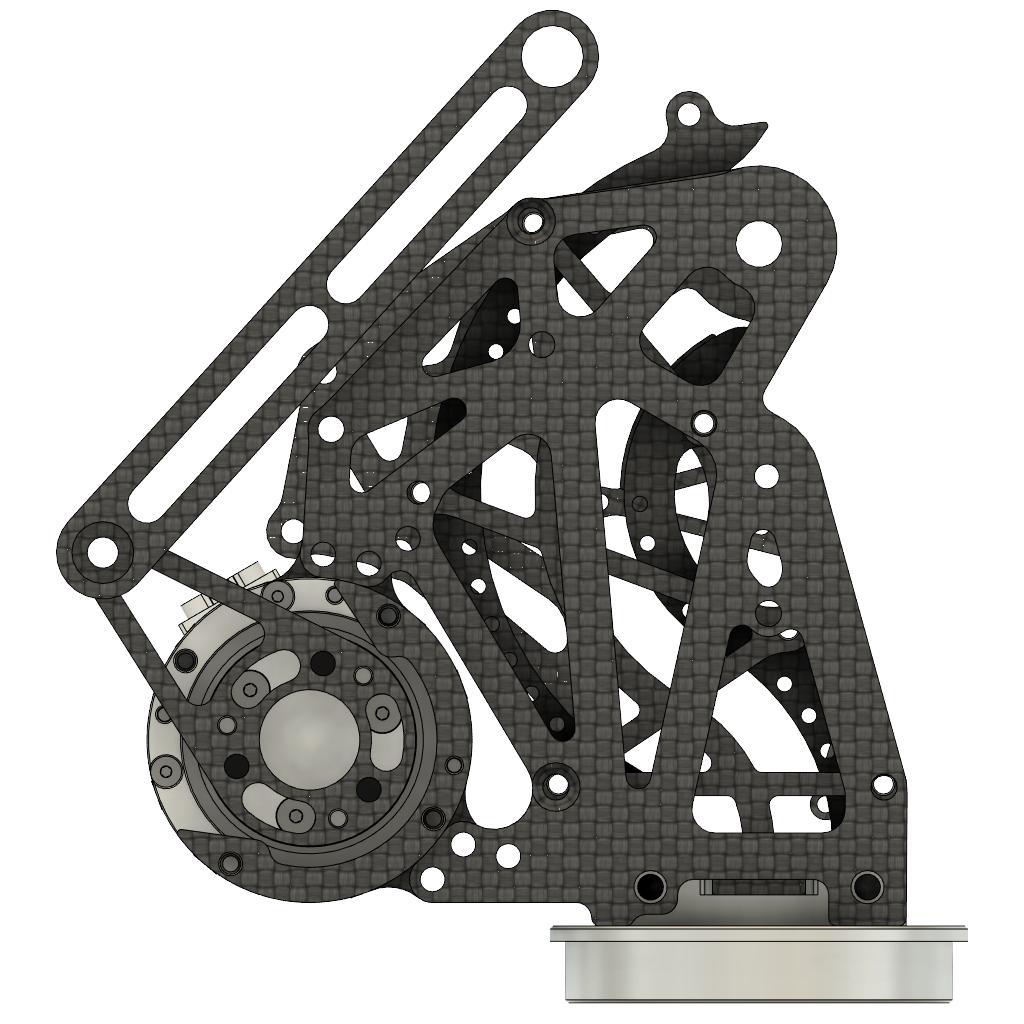
\includegraphics[width=0.6\columnwidth]{figure/设计方案/机械结构设计/云台支架侧视图 隐藏minipc和雷达.png}
        \end{minipage}
    }
    \subfigure[云台支架GM6020\label{fig:云台支架6020_设计方案}]{
        \begin{minipage}[t]{0.45\linewidth}
        \centering
        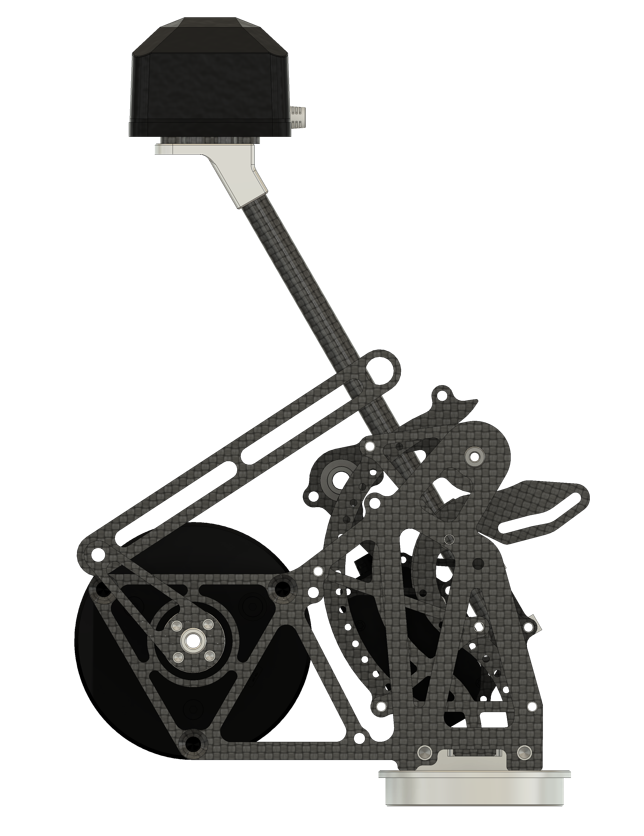
\includegraphics[width=0.6\columnwidth]{figure/设计方案/机械结构设计/云台支架GM6020.png}
        \end{minipage}
    }
    \caption{两种pitch轴驱动方式\label{fig:两种Pitch轴驱动方式_设计方案}}
\end{figure}

为提高云台响应，我们在哨兵上使用了自制的M3508云台电机，如 \figref {fig:自制M3508云台电机展示_设计方案}，该电机仅重$\qty{170}{\g}$。我们将M3508原装的减速箱替换成自制的减速箱，自制减速箱为2K-H结构，齿轮采用线切割中走丝加工制成，减速比为11。自制的M3508云台电机减速器背隙＜$\qty{30}{\arcsecond}$，徒手感知不到间隙。减速器输出端采用四点接触轴承，抗冲击性能强，并且为方便固定采用端面输出。减速后最大输出力矩约为$\qty{3}{\newton\meter}$。

该云台电机虽没有绝对位置编码器，但由于使用在Pitch轴上不需要全向转动，仅需在电机上电时旋转到限位处通过碰撞限位来确定Pitch轴初始位置，即可实现在不额外添加传感器的前提下控制云台Pitch轴。

\begin{figure}[hbt!]
    \centering
    \subfigure[M3508P11斜二测\label{fig:3508P11斜二测_设计方案} ]{
        \centering
        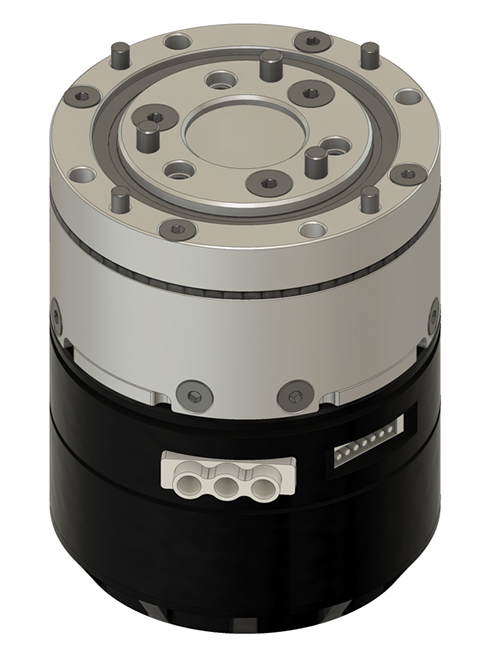
\includegraphics[width=0.2\columnwidth]{figure/设计方案/机械结构设计/M3508P11斜二测.jpg}
    }
    \subfigure[M3508P11剖面图\label{fig:3508P11剖面图_设计方案}]{
        \centering
        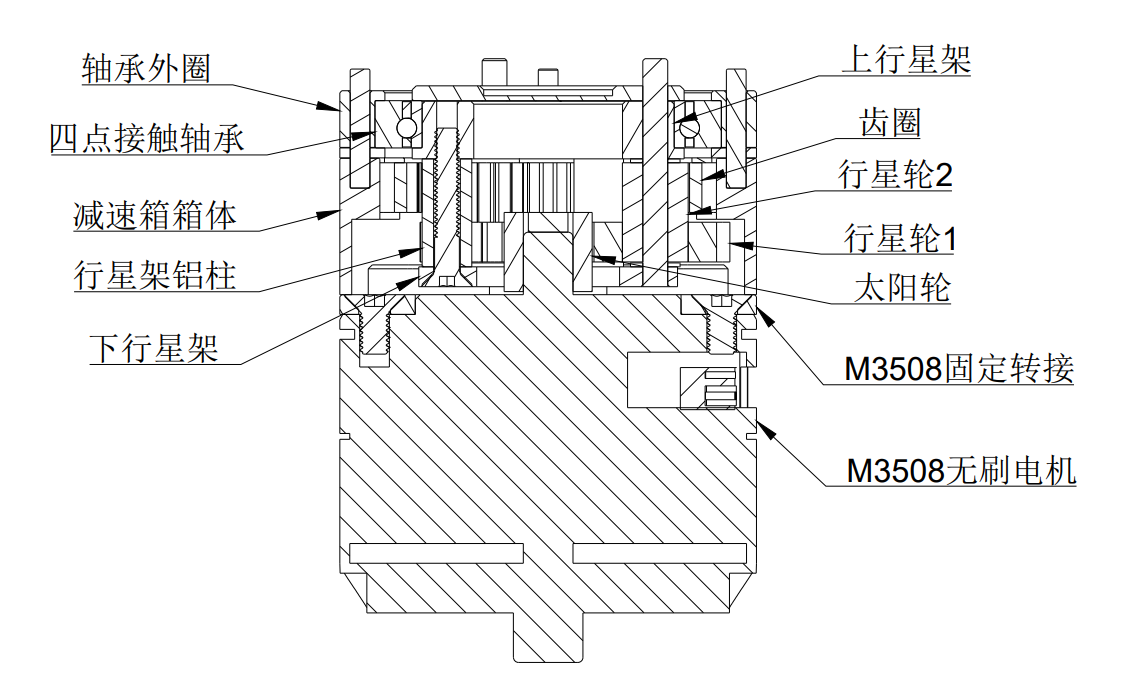
\includegraphics[width=0.48\columnwidth]{figure/设计方案/机械结构设计/M3508P11剖面图.png}
    }
    \subfigure[M3508P11实物图\label{fig:3508P11实物图_设计方案}]{
        \centering
        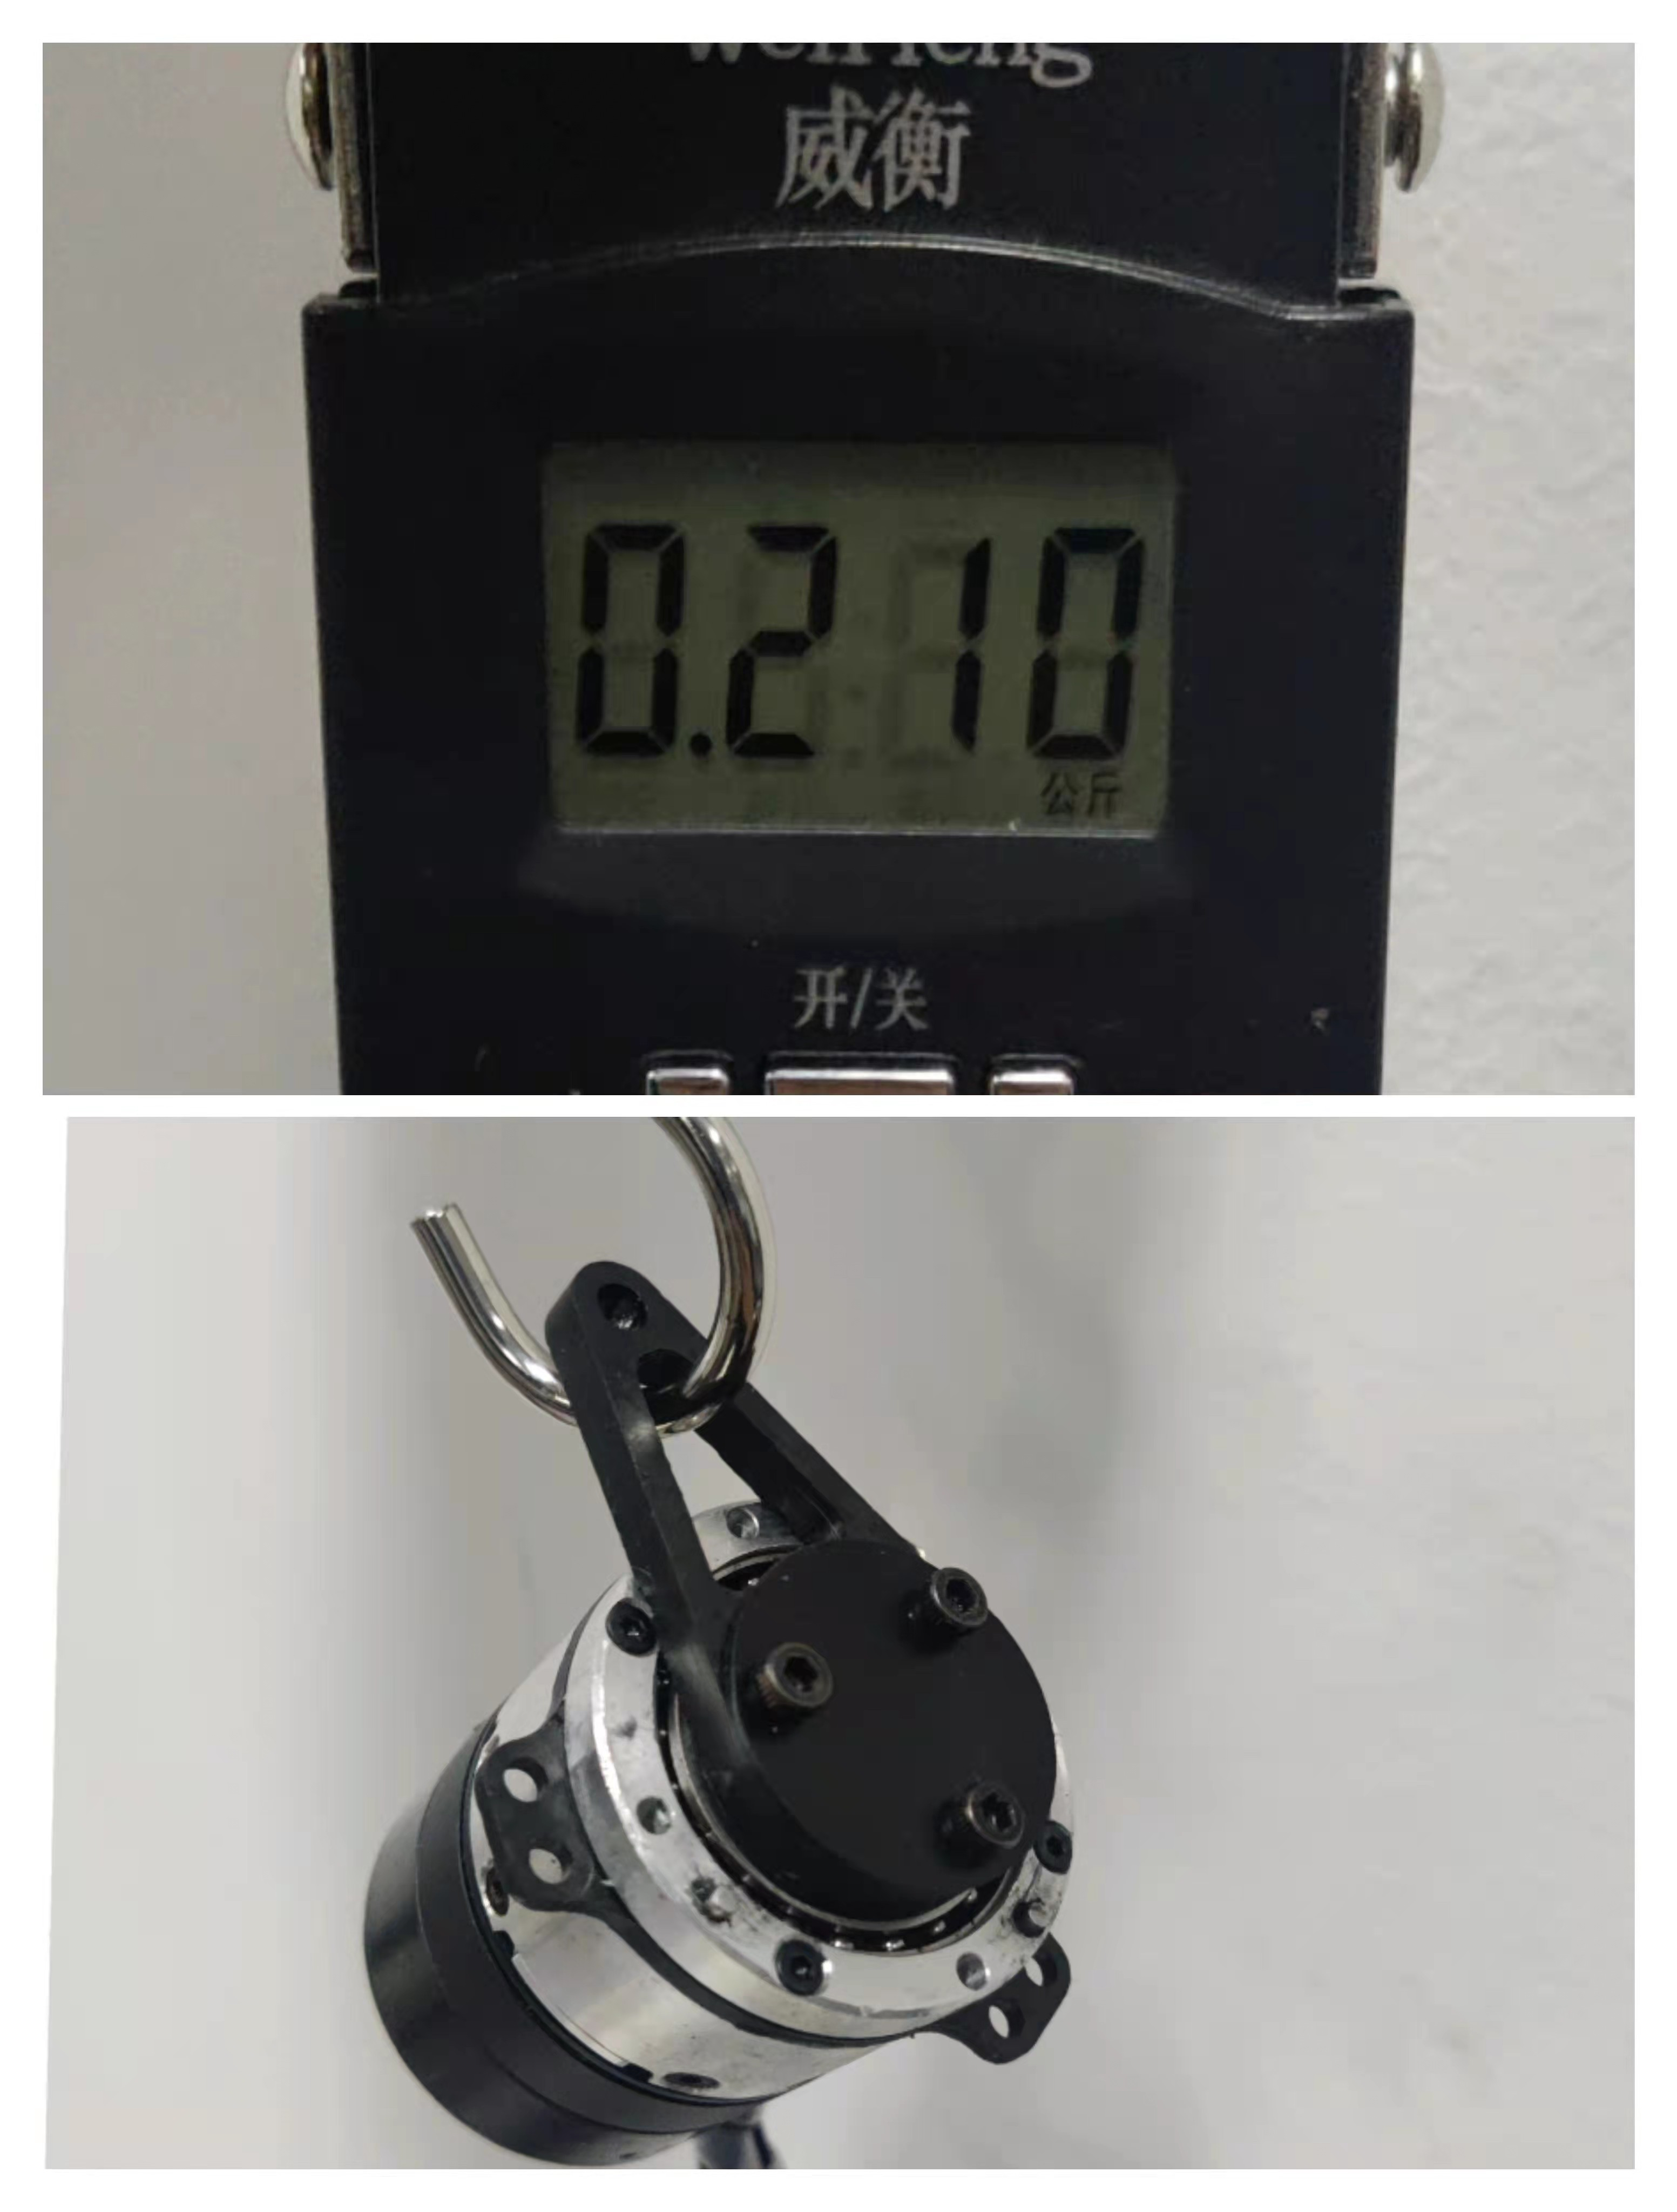
\includegraphics[width=0.2\columnwidth]{figure/设计方案/机械结构设计/M3508P11实物图.jpg}
    }
    \caption{自制M3508云台电机展示\label{fig:自制M3508云台电机展示_设计方案}}
\end{figure}



\subsubsection{发射设计}

发射结构使用M3508电机（去减速箱），摩擦轮直径$\qty{60}{\mm}$、摩擦轮中心距$\qty{73}{\mm}$、最小间距$\qty{13}{\mm}$。整体设计中将双枪转轮结构、发射枪管模块、电控模块、摄像头分模块前中后上放置，实现发射Pitch轴质心靠近转轴，同时也可单独对某模块进行拆卸维修而不影响其他模块。
 如 \figref {fig:shooter_pitch}所示。


\begin{figure}[hbt!]
     \centering
     \subfigure[发射轴测图 \label{fig:shooter_1} ]{
        \begin{minipage}[t]{0.45\linewidth}
         \centering
         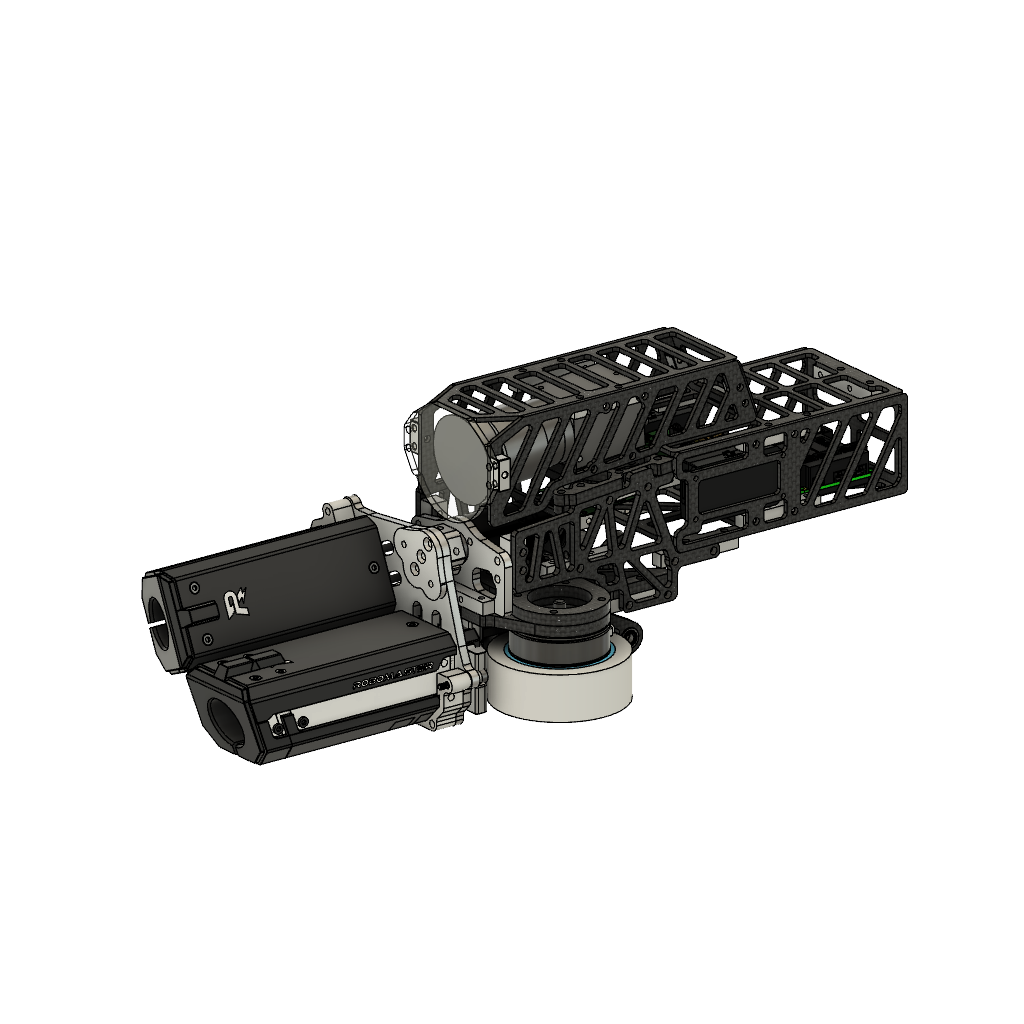
\includegraphics[width=0.8\columnwidth]{figure/设计方案/机械结构设计/发射轴测图.png}
         \end{minipage}
     }
     \subfigure[发射爆炸图\label{fig:shooter_2}]{
        \begin{minipage}[t]{0.45\linewidth}
         \centering
         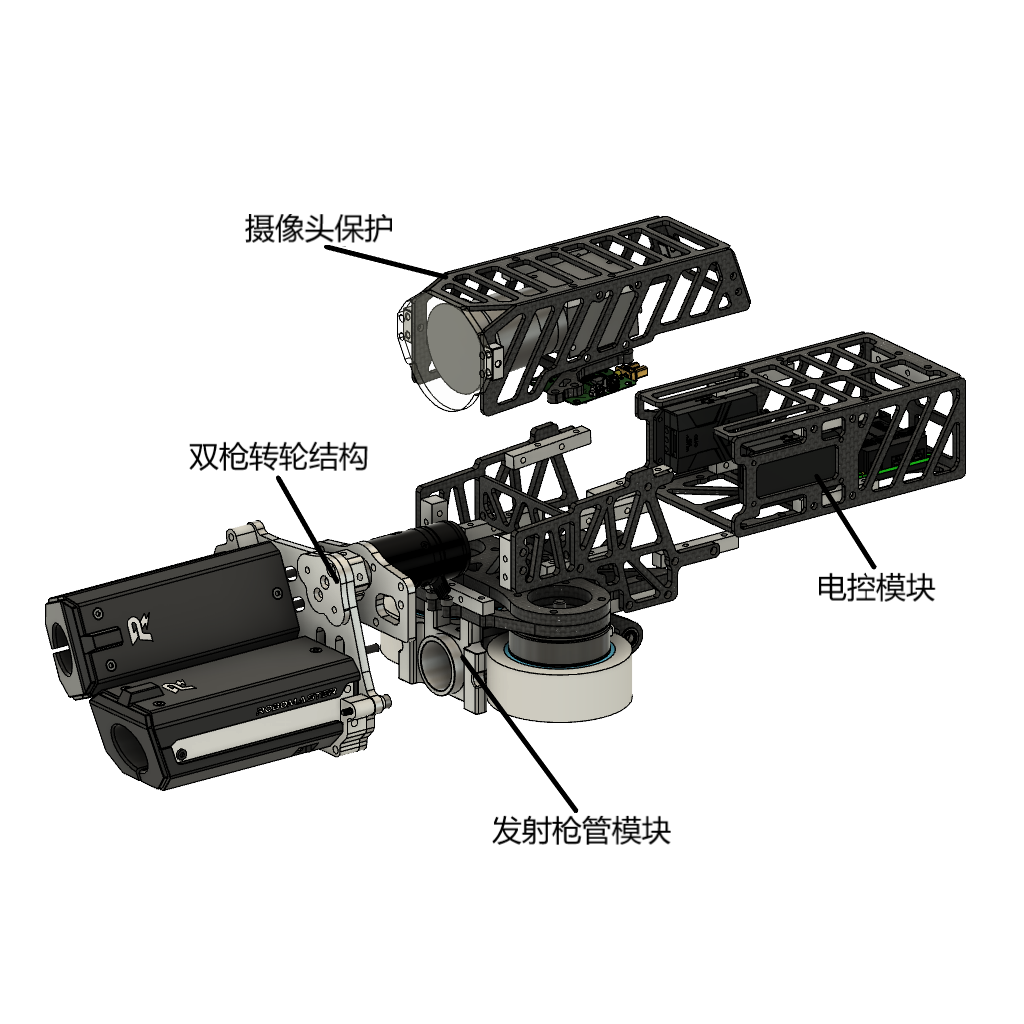
\includegraphics[width=0.8\columnwidth]{figure/设计方案/机械结构设计/发射爆炸视图.png}
         \end{minipage}
     }
     \caption{发射展示 \label{fig:shooter_pitch}}
 \end{figure}


\paragraph{枪管结构}

哨兵机器人发射系统采用6061铝合金铣削而成的一体式枪管。如 \figref{fig:原枪管展示_设计方案}所示，主体部分参考22赛季步兵机器人的设计方案：摩擦轮固定板由4个M4螺丝与铝件固定，确保摩擦轮固定板和枪管铝件的相对刚性；由于螺纹无法起到定位作用，我们在铝件上添加了两个销钉孔，确保摩擦轮固定板和枪管铝件的相对位置，进而保证了摩擦轮的定位精度；弹丸在与摩擦轮接触后枪管直径扩大，确保弹丸在加速过程中和加速后不会被外界因素干扰，避免了弹丸和枪管摩擦导致旋转。

\begin{figure}[hbt!]
    \centering
    \subfigure[原枪管斜二测图\label{fig:枪管斜二测图_设计方案} ]{
        \begin{minipage}[t]{0.45\linewidth}
        \centering
        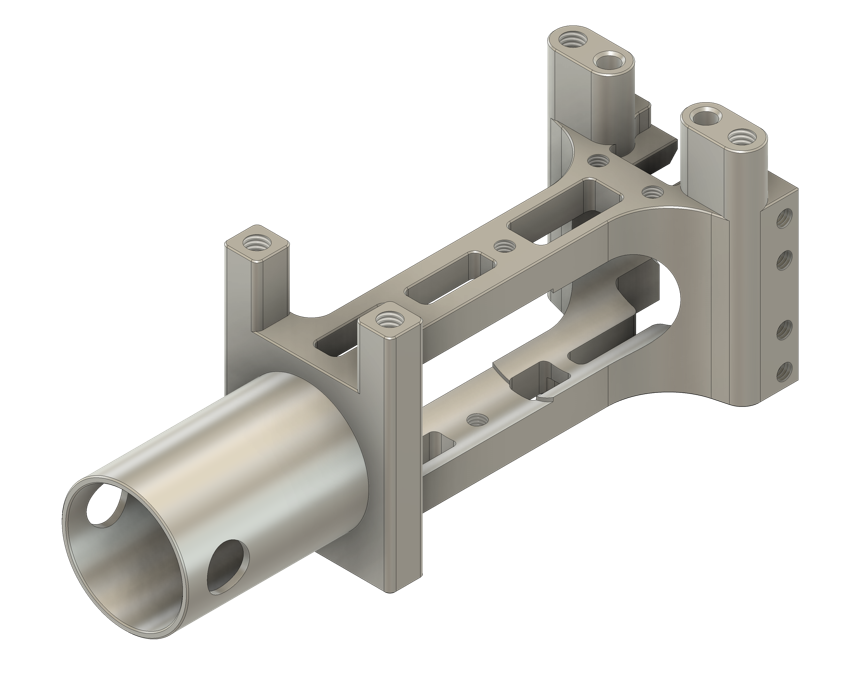
\includegraphics[width=0.8\columnwidth]{figure/设计方案/机械结构设计/原枪管斜二测视图.png}
        \end{minipage}
    }
    \subfigure[原发射机构剖面图\label{fig:发射机构剖面图_设计方案}]{
        \begin{minipage}[t]{0.45\linewidth}
        \centering
        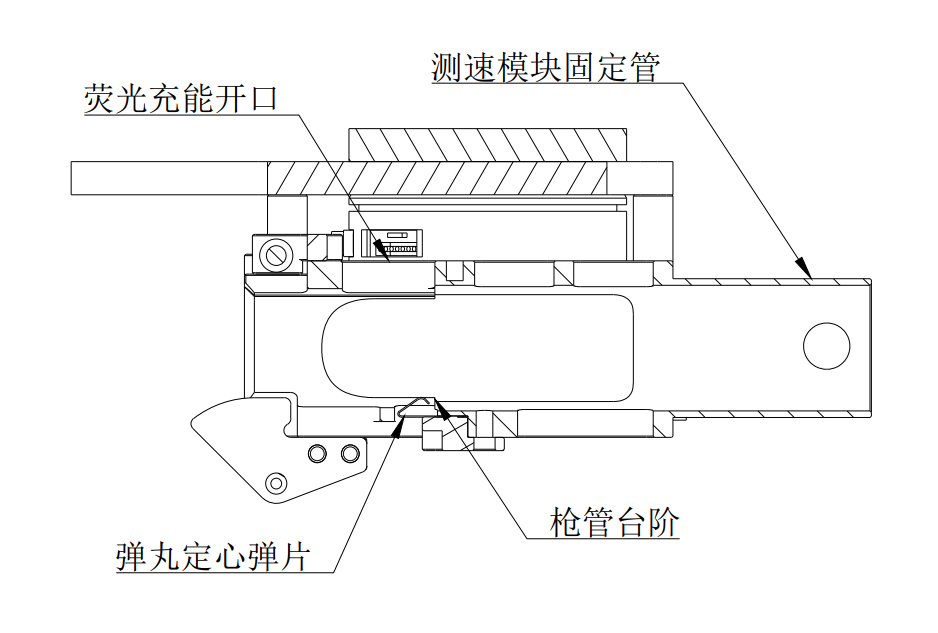
\includegraphics[width=0.8\columnwidth]{figure/设计方案/机械结构设计/原枪管剖视图.png}
        \end{minipage}
    }
    \caption{原枪管展示\label{fig:原枪管展示_设计方案}}
\end{figure}

鉴于上赛季和步兵软单发限位的不稳定性和发射散布大的问题，我们研究了各大高校单发限位相关的开源文档后，发现大部分具有出色效果的单发限位皆为硬轴承方案，于是我们决定尝试在原枪管的基础上采用轴承硬限位方案。事实上，初次对于硬限位方案进行尝试的道路注定是充满了曲折的。

因为滑槽下供弹枪管的特殊性，我们参考了各大高校开源出来上下双轴承的距离参数后，在第一版测试枪管的设计上采用模拟相同的距离参数、上轴承下定心滑轨的结构来避免干涉问题。

首先，遇到的问题就是我们购买的开式U型轴承自身定子和转子的刚性并不良好，于是我们购买了刚性好上不少的闭式U型轴承，尽量避免轴承自身刚性问题对发射重复度所存在的影响。

其次，由于经济原因和对较快迭代速度的要求我们采用了PLA打印件作为测试枪管，这会导致原本以作为6061铝合金材料枪管的设计在强度和刚度上是不能满足PLA枪管在测试过程中对强度和刚度的要求的，于是我们额外设计了加厚、去减重的一系列测试枪管3D模型并设立新的文件夹方便管理和版本迭代或者回溯，在取得稳定良好的发射重复度之前我们舍弃了荧光充能和测速模块的固定设计。

最后，在不断测试第一版单轴承测试枪管的时间里，我们经常发现卡弹和双发并存的现象。这是由于卡弹所以导致前一发弹丸直到被后一发弹丸推出单发限位后才成功发射，这才出现了双发现象。我们也尝试减小挤压量不断测试，发现发射不卡弹时的挤压量必定会导致弹丸大概率的双发，同时发射的重复度也越来越差，我们可以判定此时单发限位实际上已经没有正常地起到让弹丸单发的限位作用了。第一版枪管的最终设计方案如 \figref{fig:第一版枪管展示_设计方案}所示。


\begin{figure}[hbt!]
    \centering
    \subfigure[第一版枪管斜二测图\label{fig:第一版枪管斜二测图_设计方案} ]{
        \begin{minipage}[t]{0.45\linewidth}
        \centering
        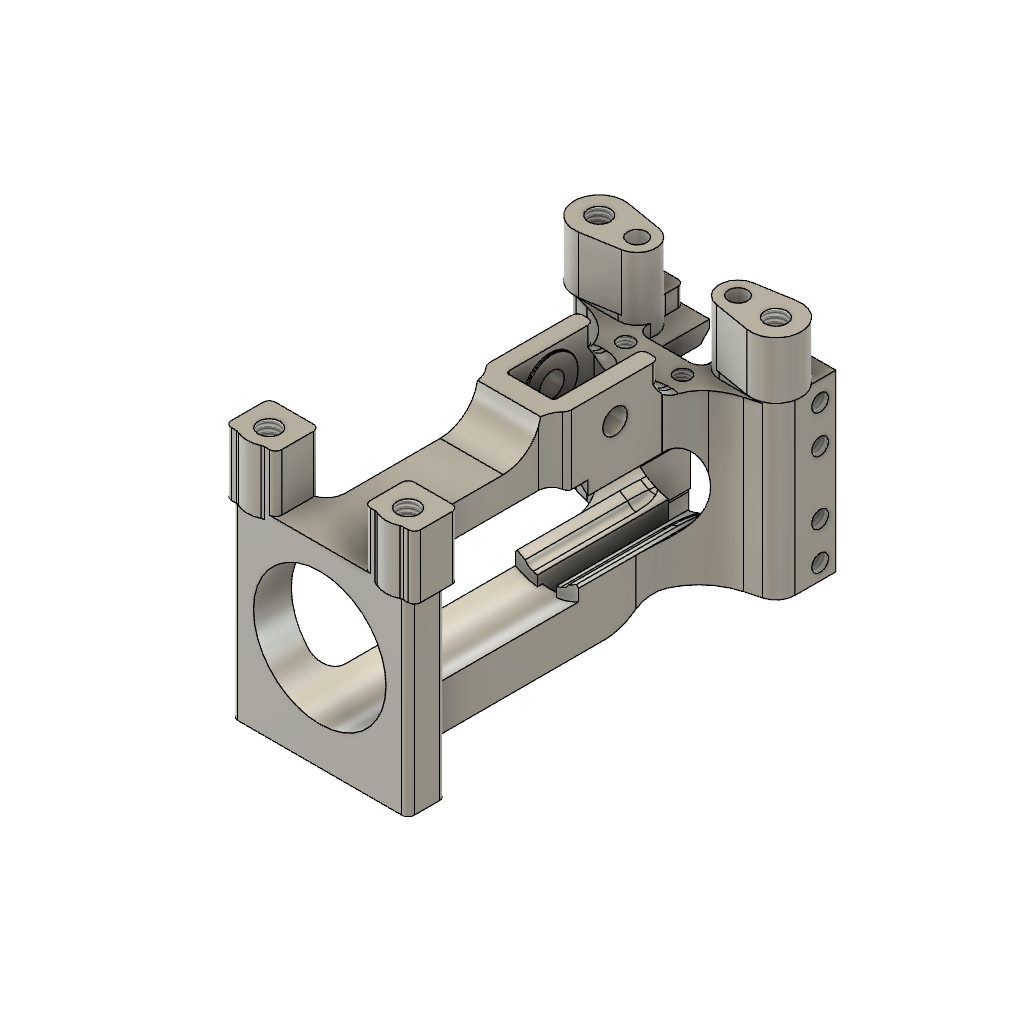
\includegraphics[width=0.8\columnwidth]{figure/设计方案/机械结构设计/第一版枪管轴侧图.png}
        \end{minipage}
    }
    \subfigure[第一版发射机构剖面图\label{fig:第一版发射机构剖面图_设计方案}]{
        \begin{minipage}[t]{0.45\linewidth}
        \centering
        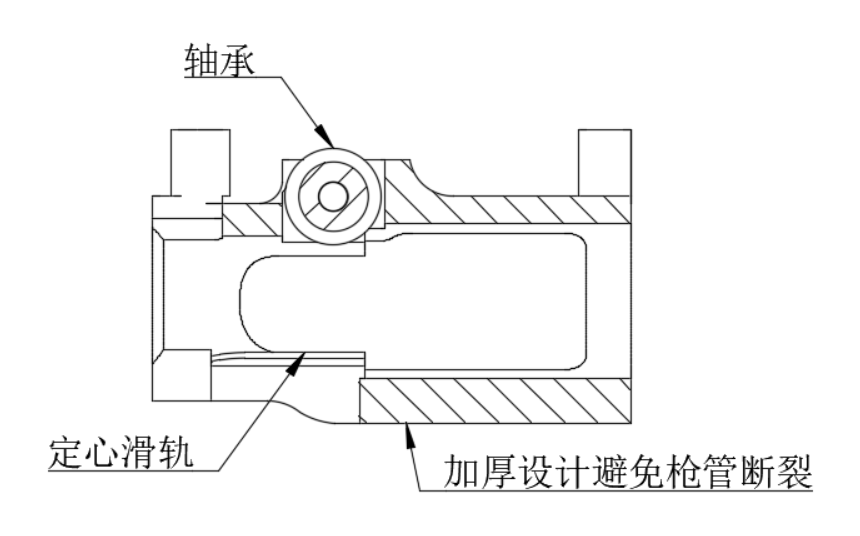
\includegraphics[width=0.8\columnwidth]{figure/设计方案/机械结构设计/第一版枪管剖视图.png}
        \end{minipage}
    }
    \caption{第一版枪管展示\label{fig:第一版枪管展示_设计方案}}
\end{figure}

我们锁定第一版上轴承枪管最大的问题，是单发限位对于弹丸阻力过大。在第二版测试枪管上采用上下双轴承的单发限位结构，用上下同时的滚动摩擦替代单侧滚动摩擦单侧滑动摩擦，同时进行了枪管长度的延长来解决原有的干涉问题，通过和控制组队员一起调整拨盘初始位置偏移量这一参数来解决弹道加长导致的弹丸不能正确地接触单发限位的问题。经观察对比第一版和第二版的枪管表现，我们发现在弹丸挤压量相同时，上轴承枪管对弹丸的阻力远远大于第二版枪管对弹丸的阻力。这既验证了我们的想法，也说明了上轴承下定心滑轨的结构在这样的设计下，是不合格的单发限位。

在我们更换成如 \figref {fig:第二版枪管展示_设计方案}所示的第二版双轴承方案后，弹丸卡弹的问题得到了解决，重复度也有所提高。在此过程中，我们虽然测试了不同的弹丸挤压量，但是发现这些推荐参数并不能达到预期效果，因此我们必须探究究竟还有哪部分的参数会影响发射的重复度。此时广城理的同学提出弹丸刚离开单发限位时位置球心处和摩擦轮中心轴在枪管侧视图上的投影距离对于发射重复度的重要性（也可以简单理解为单发限位到摩擦轮中心轴在枪管侧视图上的投影距离），启发了我们去完善这方面的知识储备。测试结果也证明，合适的弹丸刚离开单发限位时位置球心处和摩擦轮中心距在枪管侧视图上的投影距离可以改善发射重复度。

\begin{figure}[hbt!]
    \centering
    \subfigure[第二版枪管斜二测图\label{fig:第二版枪管斜二测图_设计方案} ]{
        \begin{minipage}[t]{0.45\linewidth}
        \centering
        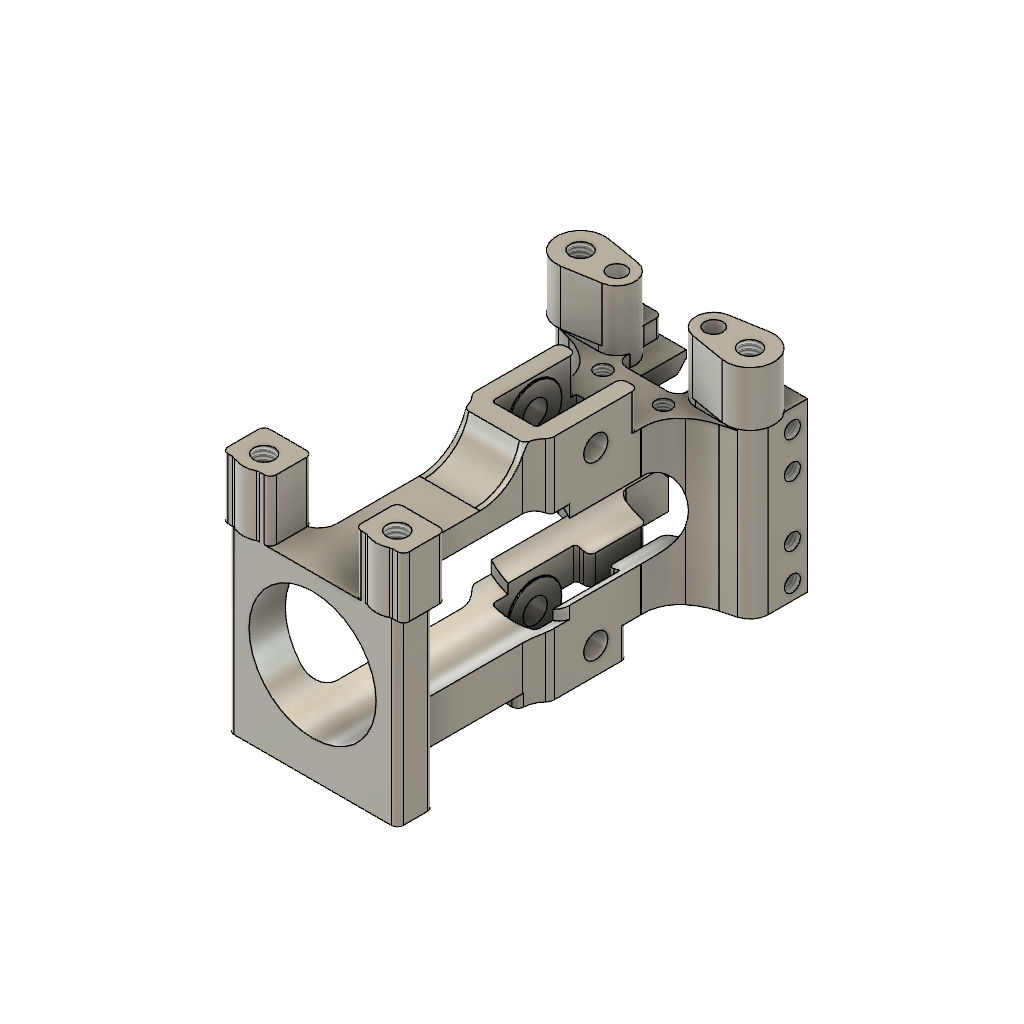
\includegraphics[width=0.8\columnwidth]{figure/设计方案/机械结构设计/第二版枪管轴测图.png}
        \end{minipage}
    }
    \subfigure[第二版发射机构剖面图\label{fig:第二版发射机构剖面图_设计方案}]{
        \begin{minipage}[t]{0.45\linewidth}
        \centering
        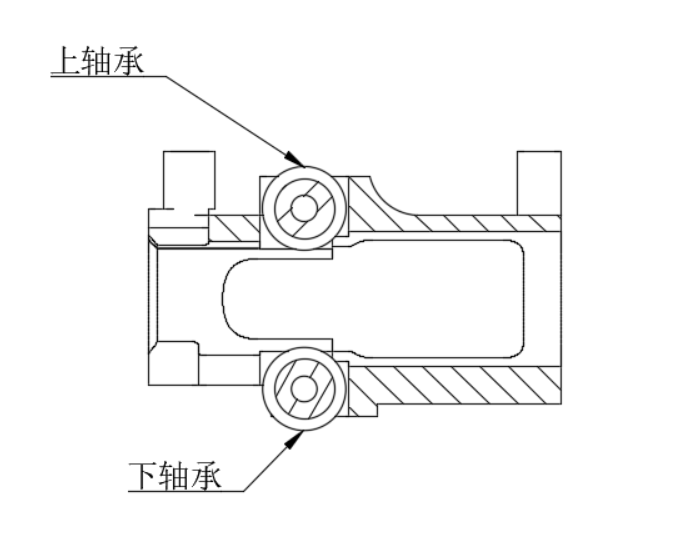
\includegraphics[width=0.8\columnwidth]{figure/设计方案/机械结构设计/第二版枪管剖视图.png}
        \end{minipage}
    }
    \caption{第二版枪管展示\label{fig:第二版枪管展示_设计方案}}
\end{figure}

在多次测试都无法复现技术开源报告中相同方案甚至是相同参数枪管的发射效果后，我们用上供弹结构的发射系统做了验证，发现得益于上供弹简单的弹链，具有相同关键参数的枪管可以较为成功地复现到技术开源报告里描述的发射效果。于是我们发出了“对于下供弹机构是否适合硬限位”这一疑问。

由于时间紧迫，我们马上启用了如 \figref {fig:第三版枪管展示_设计方案}所示第三版测试枪管，用回了21赛季前辈们已经做出良好效果的拉簧软限位。在测试过一系列挤压量、拉簧的弹簧丝系数和长度后，我们得到了一千发以内双发0-1次、$\qty{5}{\mm}$发射重复度可以做到小装甲板以内的散布的发射测试结果。

\begin{figure}[hbt!]
    \centering
    \subfigure[第三版枪管斜二测图\label{fig:第三版枪管斜二测图_设计方案} ]{
        \begin{minipage}[t]{0.45\linewidth}
        \centering
        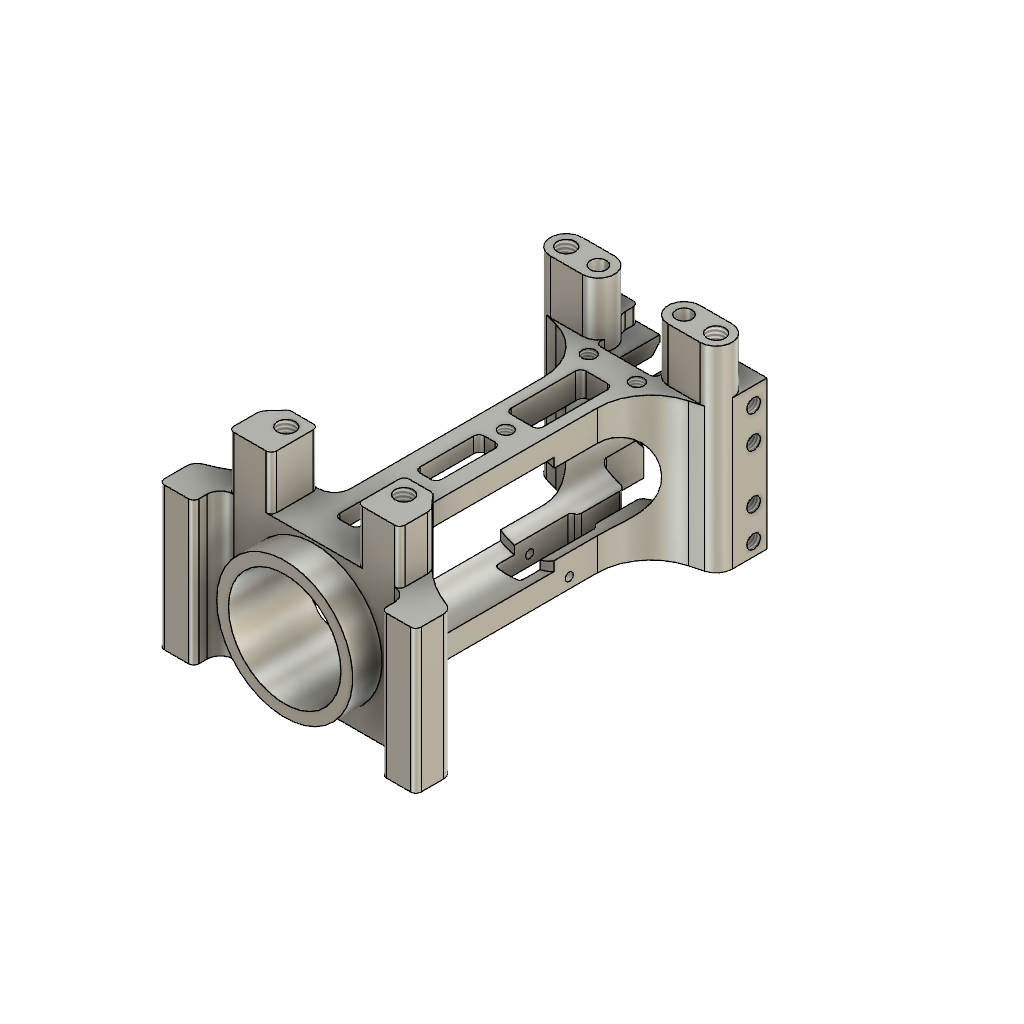
\includegraphics[width=0.8\columnwidth]{figure/设计方案/机械结构设计/第三版枪管轴二测图.png}
        \end{minipage}
    }
    \subfigure[第三版发射机构剖面图\label{fig:第三版发射机构剖面图_设计方案}]{
        \begin{minipage}[t]{0.45\linewidth}
        \centering
        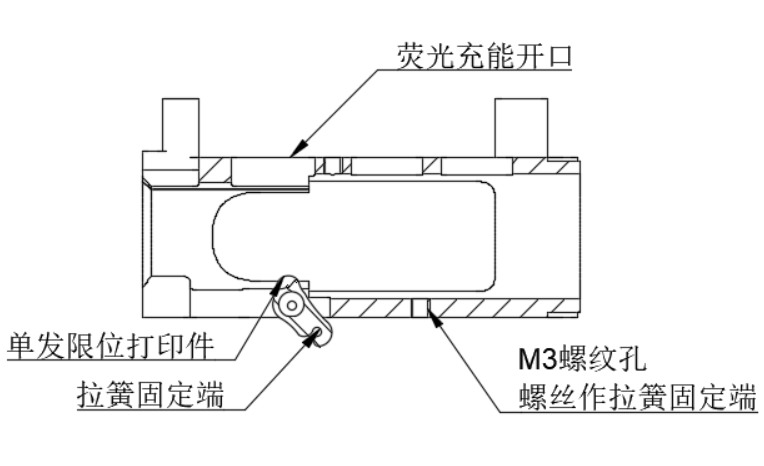
\includegraphics[width=0.8\columnwidth]{figure/设计方案/机械结构设计/第三版枪管剖视图.png}
        \end{minipage}
    }
    \caption{第三版枪管展示\label{fig:第三版枪管展示_设计方案}}
\end{figure}

% \newpage
\paragraph{弹丸定心结构}

哨兵机器人的弹丸定心结构的设计是为了保证弹丸每次与摩擦轮在同一位置接触，从而获得较高的发射精度。
在这个赛季，我们探究了三种弹丸定心方案，并且不断完善。

最开始的方案一的本质就是直接让单发限位机构发挥全部的弹丸定心作用。

如\figref {fig:弹丸定心结构_设计方案一}所示方案一与第一版枪管配合使用，我们赋予了上轴承下定心滑轨结构两个使命———单发限位和弹丸定心。在方案一中，弹丸从待发位置到与摩擦轮接触前，弹丸会被单发限位的上轴承向下顶在两条定心滑轨之间，形成四点定位。然而我们在测试的时候发现，挤压量太大时弹丸会卡死在单发限位处，挤压量太小时根本限制不住弹丸。

伴随着第二版枪管投入测试，我们一开始也并没有分隔开单发限位机构和弹丸定心机构，直到我们意识到：如果保证弹丸每次与单发限位在同一位置接触，那么更有利于保证弹丸每次与摩擦轮在同一位置接触。

因此我们提出了如\figref {fig:弹丸定心结构_设计方案二}所示的方案二，弹丸从进入枪管到与单发限位接触前，弹丸会被上下四条定心滑轨约束在直径只有$\qty{17.4}{\mm}$的轨道里、弹丸从待发位置到与摩擦轮接触前，弹丸会被单发限位的上下U型轴承挤压，形成四点定位。经测试发现，增加额外的弹丸定心结构确实可以提高重复度。

为了探索弹丸定心结构提高发射重复度的极限，我们从英雄组借鉴他们的发射经验，改成如\figref {fig:弹丸定心结构_设计方案三}所示的方案三——类方形枪管入口，进行一系列长宽系数的尝试测试，并在测试过程中，与弹丸有较多接触的地方使用有润滑效果的特氟龙胶带贴纸替代粗糙的打印件内壁。最终得出，在左右$\qty{17.1}{\mm}$贴两层特氟龙胶带贴纸、上下$\qty{17.8}{\mm}$无特氟龙胶带贴纸的时候定心效果最好。

\begin{figure}[hbt!]
    \centering
    \subfigure[方案一\label{fig:弹丸定心结构_设计方案一} ]{
        \centering
        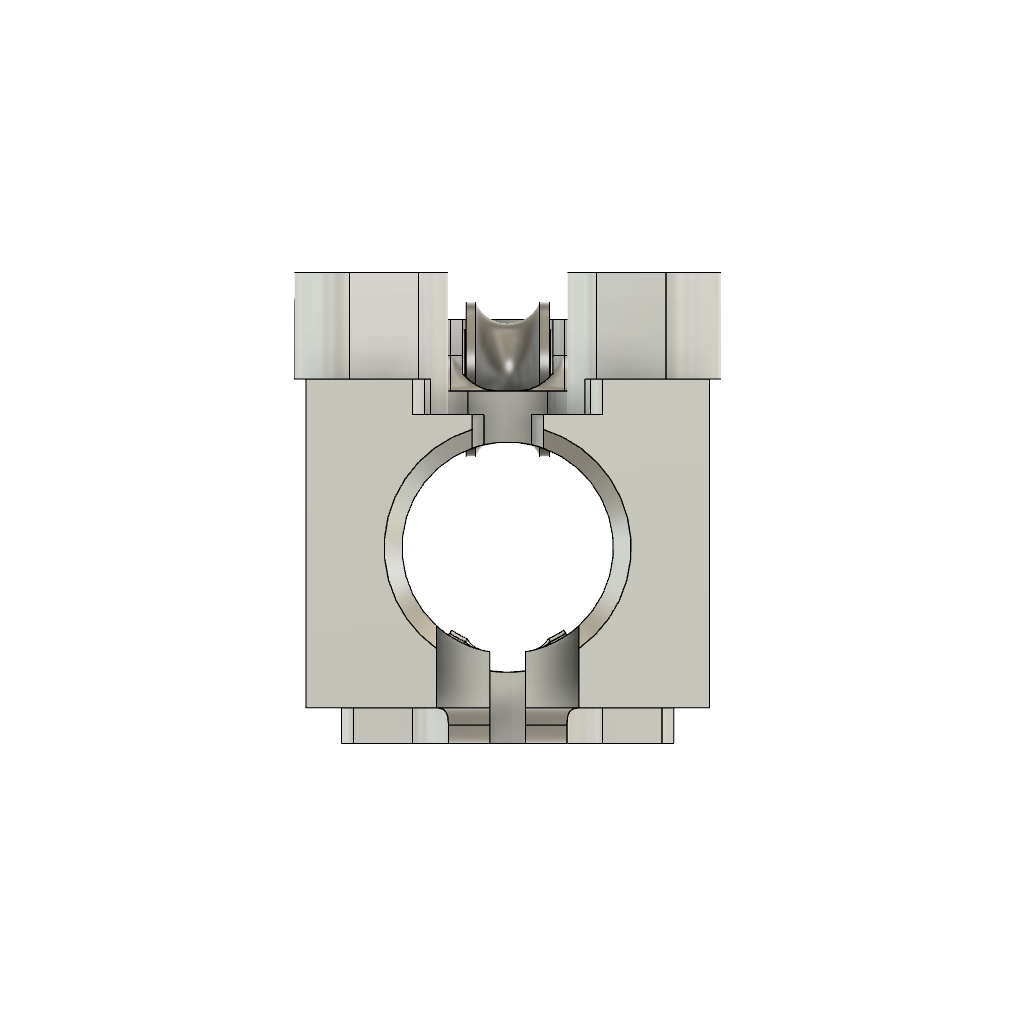
\includegraphics[width=0.3\columnwidth]{figure/设计方案/机械结构设计/1号限位.png}
    }
    \subfigure[方案二\label{fig:弹丸定心结构_设计方案二}]{
        \centering
        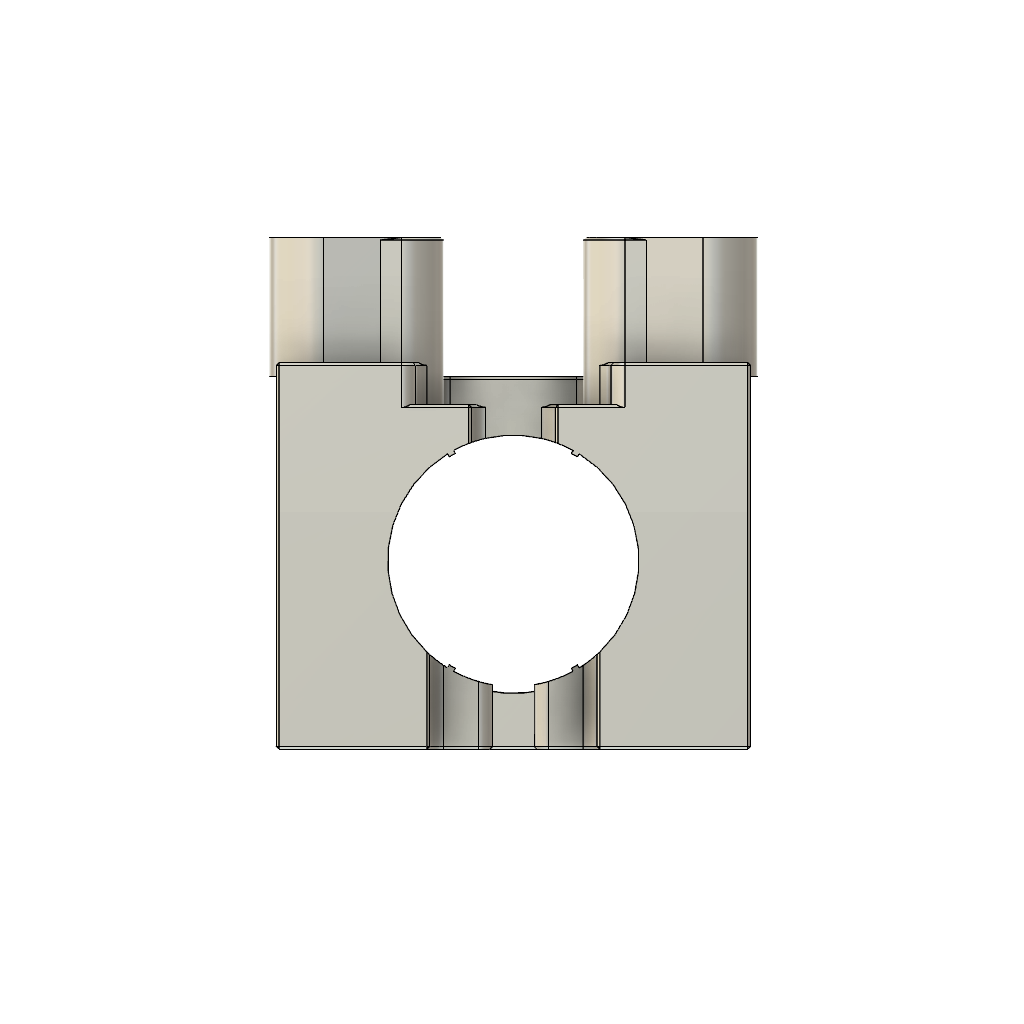
\includegraphics[width=0.3\columnwidth]{figure/设计方案/机械结构设计/2号限位.png}
    }
    \subfigure[方案三\label{fig:弹丸定心结构_设计方案三} ]{
        \centering
        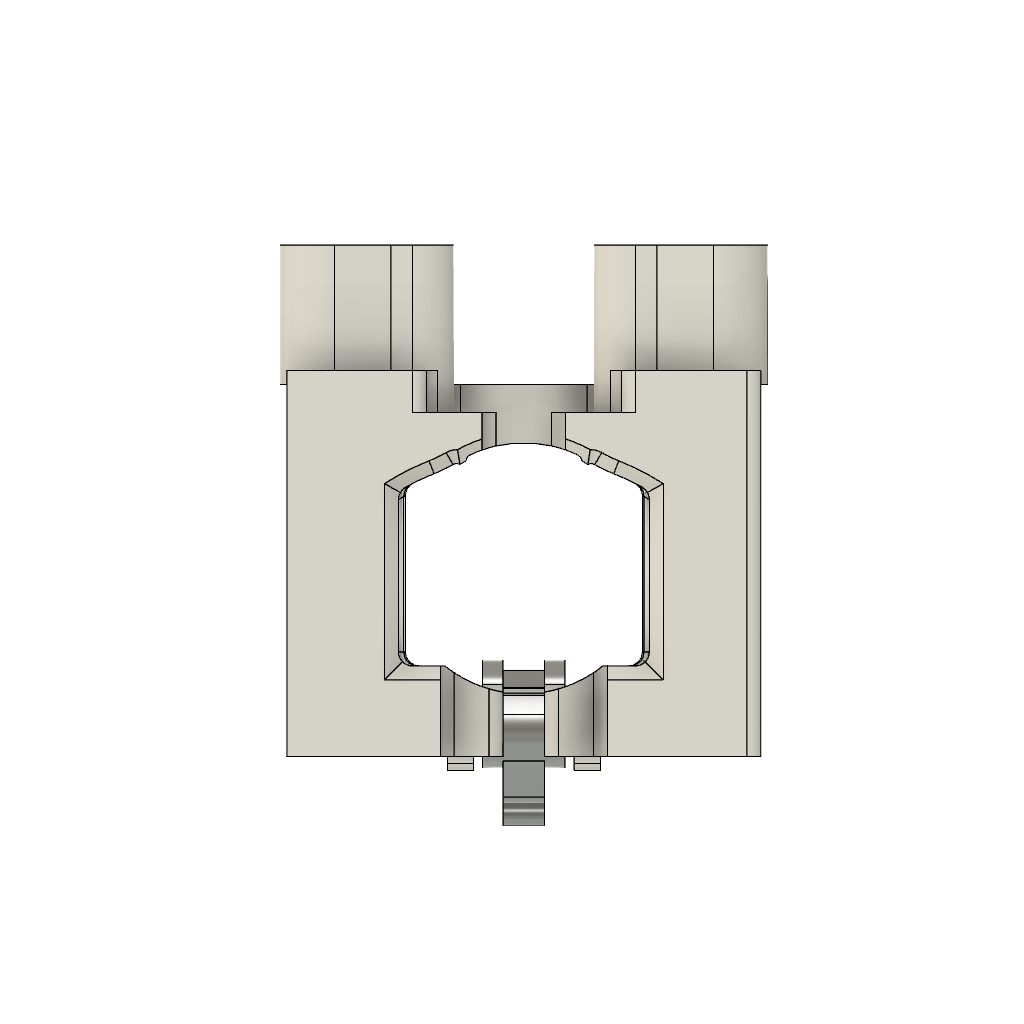
\includegraphics[width=0.3\columnwidth]{figure/设计方案/机械结构设计/3号限位.png}
    }
    \caption{弹丸定心结构展示\label{fig:弹丸定心结构展示_设计方案}}
\end{figure}

\paragraph{双枪转轮机构}

如 \figref {fig:双枪1_设计方案}
所展示，参考借鉴哈尔滨工程大学平衡步兵的双枪转轮机构\cite{RM2022哈工程:online}，采用一个M2006电机驱动的小角度转轮机构完成测速模块替换功能。对比固定式双枪管哨兵，该机构发射时产生的后坐力对Yaw轴和Pitch轴产生扭矩更小，便于进行自瞄射击。只需在单枪管哨兵云台的基础上做出极小的结构调整，不需要对云台进行大范围修改，整体结构仍保留了普通云台极低转动惯量的特性。转轮机构使用了推力滚针轴承，相比推力球轴承，其轴向载荷能力更大，刚性更好，同时占用轴向空间更小。


% 测速固定板原本采用玻纤板材，在测试过程中发现玻纤板的刚度稍不足，于是换成铝板。

如 \figref {fig:双枪2_设计方案}
所展示，在测速固定板与电机的连接固定处增加了一个压紧定位板，通过螺丝压紧将测速固定板、轴承、联轴器、电机固定板等一一紧贴，保证转轮机构的转动稳定，减小因间隙处松动带来的误差影响。

如 \figref {fig:双枪3_设计方案}
所展示，双枪定位塞打处原设计为塞打头圆柱面与一体式枪管的竖直平面平面接触撞击作为机械限位，后将一体式枪管左右两端挖出一个与定位塞打圆柱面紧贴的半圆柱槽，由原本圆柱面与平面的线接触优化为圆柱面与圆柱面的面接触限位，可以提高定位的准确度，同时也分散了塞打撞击一体式枪管时的冲击力，减小撞击接触对枪管及定位塞打的损害，以更好保证定位准确度。

\begin{figure}[hbt!]
    \centering
    \subfigure[双枪转轮机构展示 \label{fig:双枪1_设计方案} ]{
        \centering
        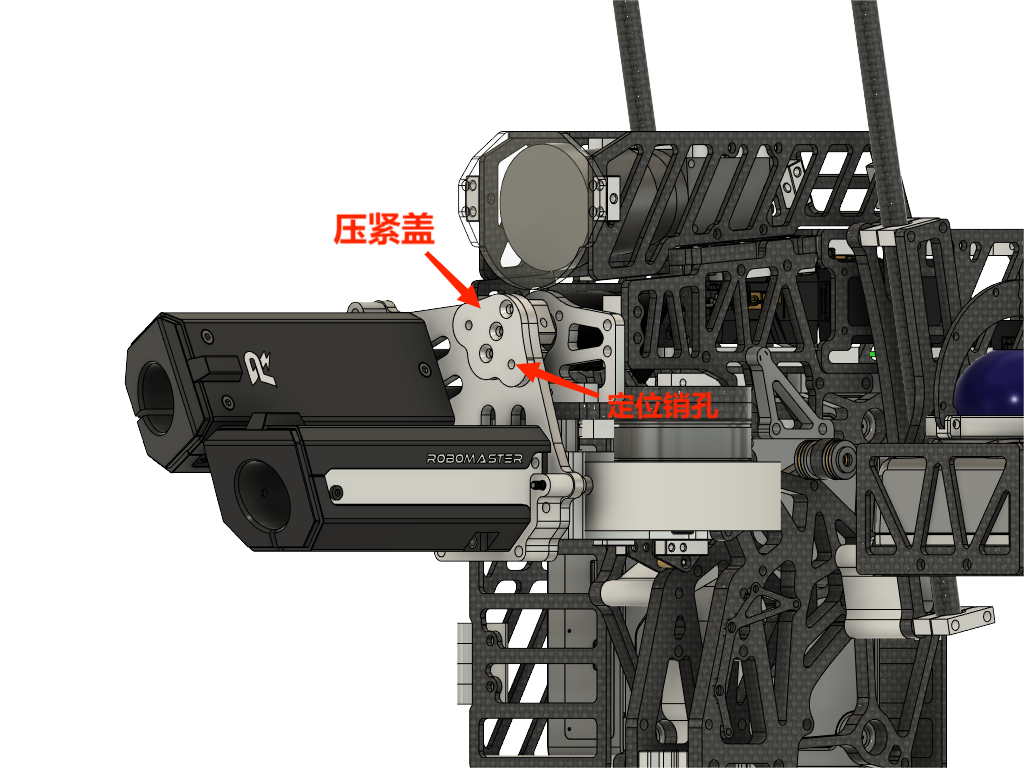
\includegraphics[width=0.4\columnwidth]{figure/设计方案/机械结构设计/双枪转轮机构.png}
    }
    
    \subfigure[双枪转轮机构侧视图\label{fig:双枪2_设计方案}]{
        \centering
        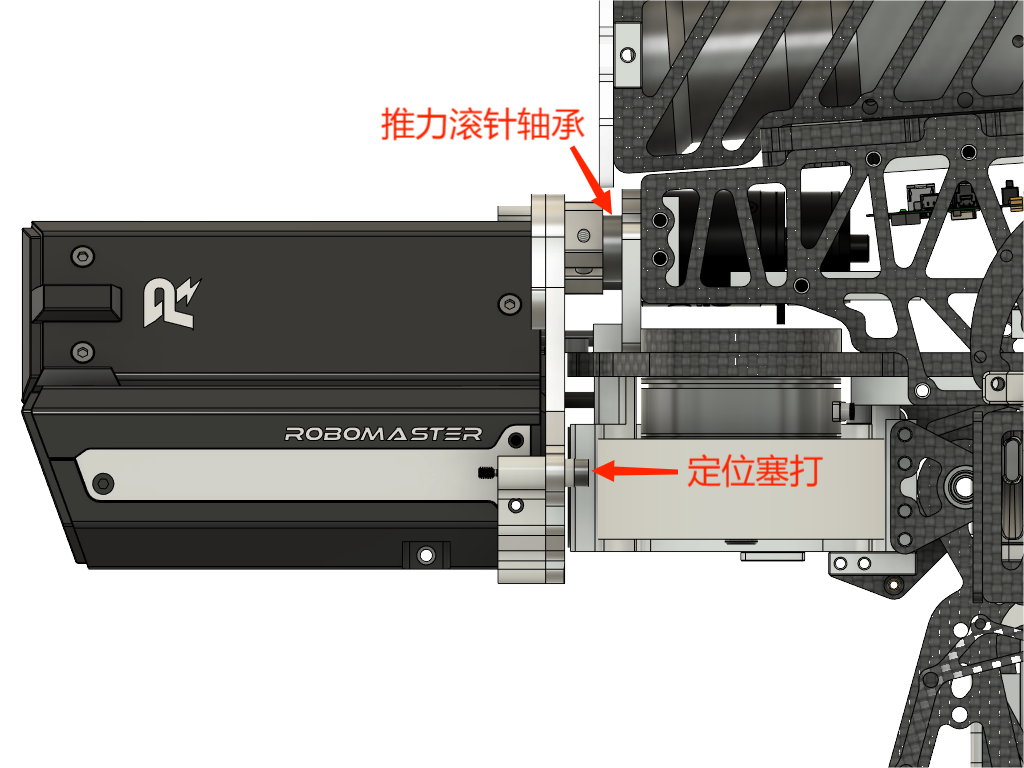
\includegraphics[width=0.35\columnwidth]{figure/设计方案/机械结构设计/双枪转轮机构侧视图.png}
    }
    \subfigure[双枪定位示意图\label{fig:双枪3_设计方案} ]{
        \centering
        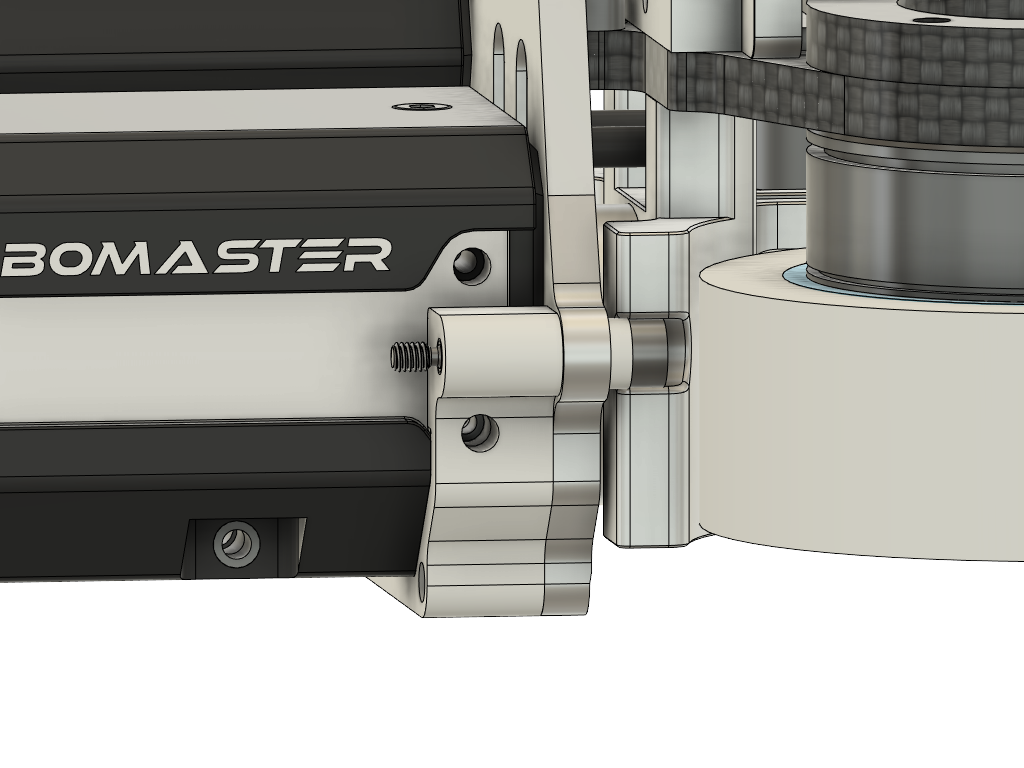
\includegraphics[width=0.35\columnwidth]{figure/设计方案/机械结构设计/双枪定位示意图.png}
    }
    \caption{双枪转轮机构展示 \label{fig:双枪_设计方案}}
\end{figure} 

\subsubsection{中心供弹设计}

\paragraph{拨盘结构}


为减小哨兵两侧轮间距，提高陀螺速度，缩短链路长度，实现哨兵轻量化，降低重心等一系列考虑，我们在北京理工大学和哈工大开源中心供弹的基础上研发了小弹丸的中心供弹拨盘。
如\figref{fig:中心供弹_设计方案}所示
 
\begin{figure}[hbt!]
   \centering
   \subfigure[底盘剖面图]{
        \begin{minipage}[t]{0.45\linewidth}
       \centering
       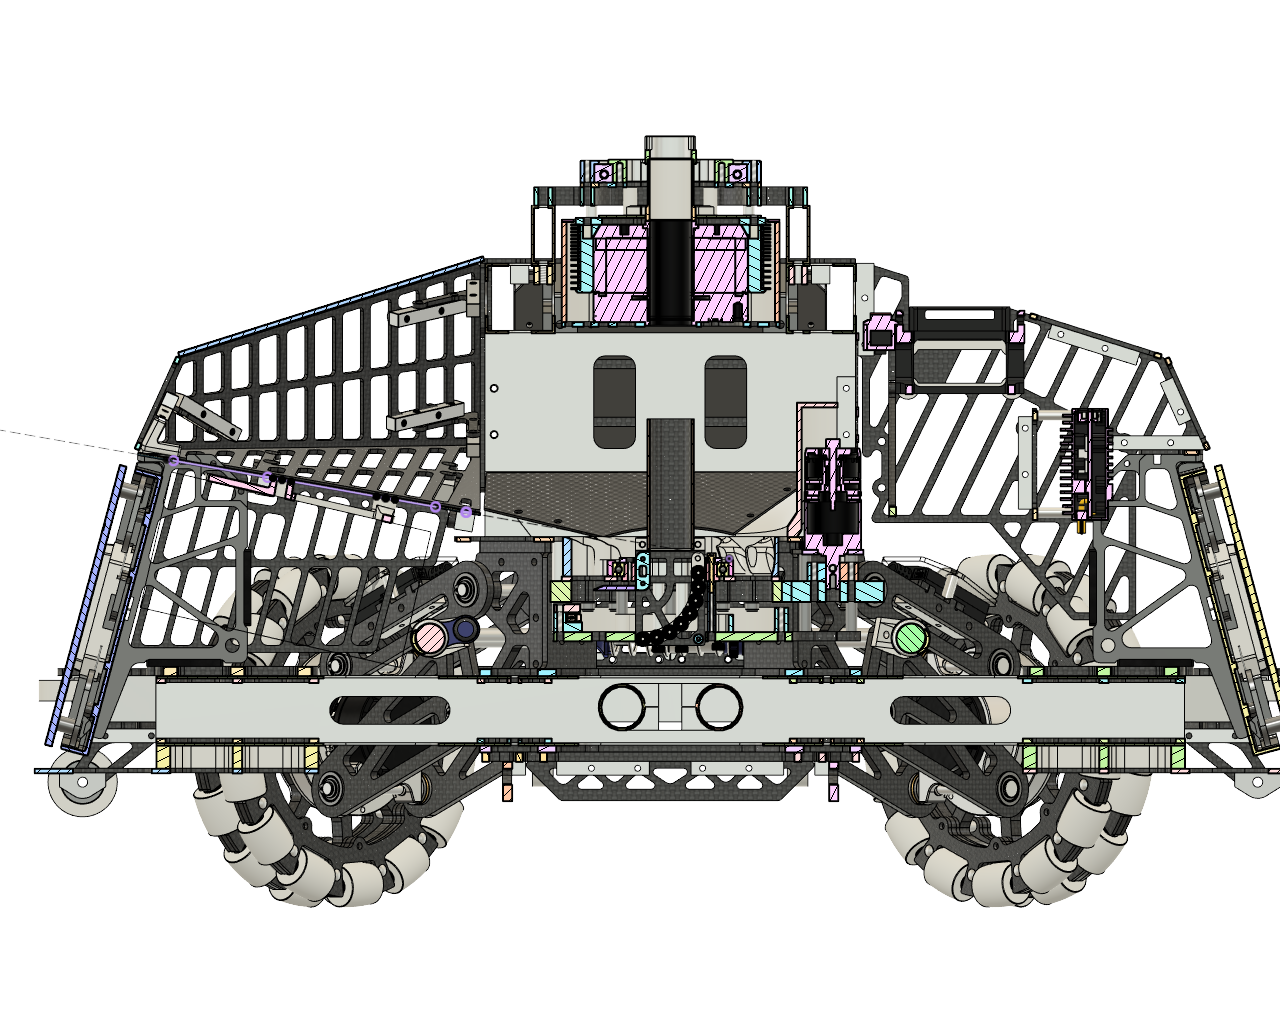
\includegraphics[width=0.7\columnwidth]{figure/设计方案/机械结构设计/底盘剖面图.png}
       \end{minipage}
   }
   \subfigure[中心供弹斜二测图]{
        \begin{minipage}[t]{0.45\linewidth}
       \centering
        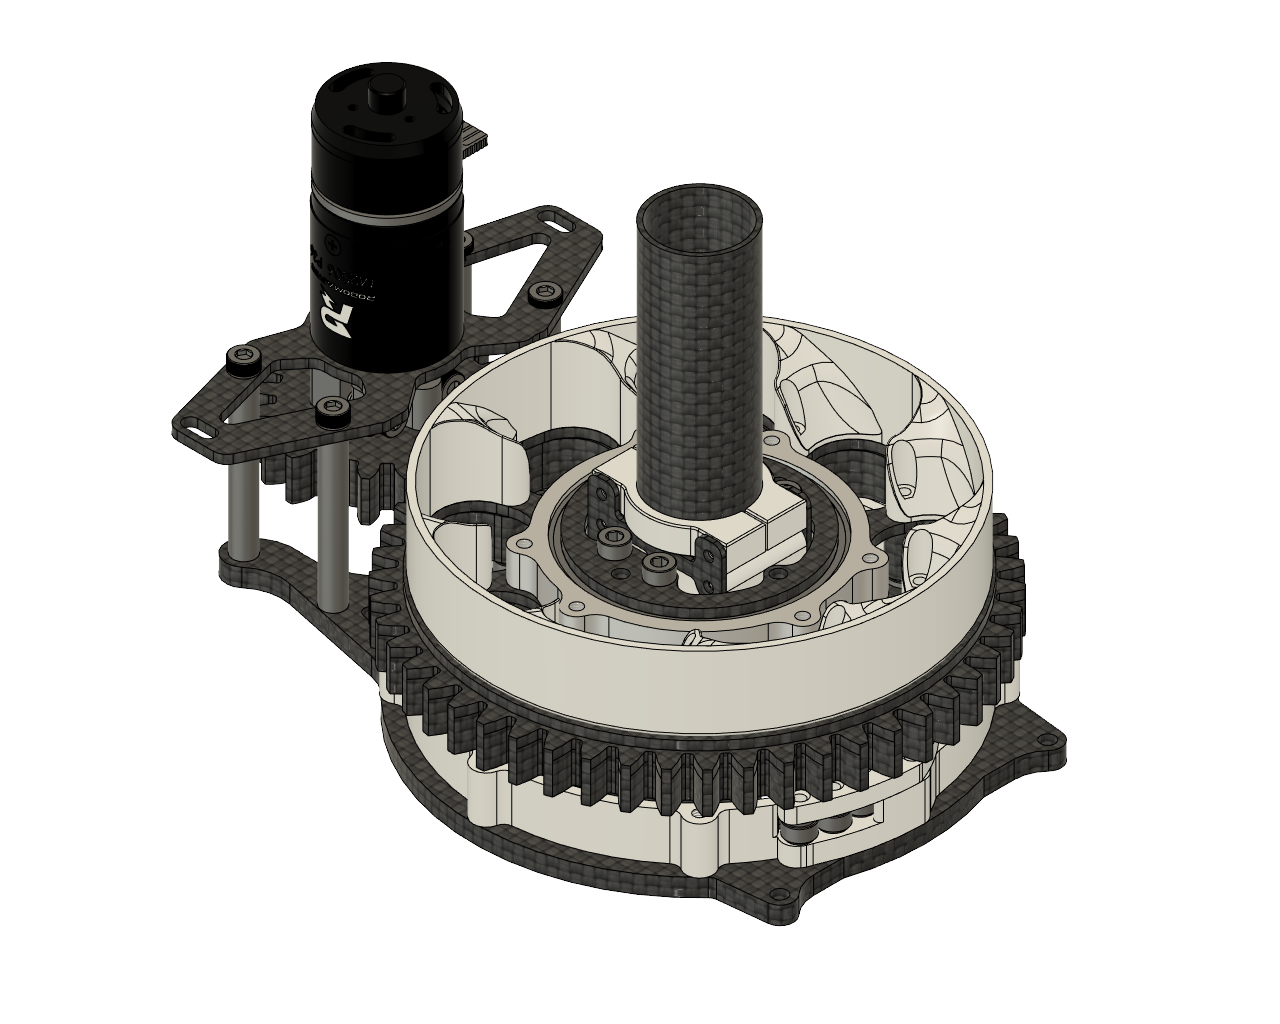
\includegraphics[width=0.7\columnwidth]{figure/设计方案/机械结构设计/中心供弹斜二测图}
        \end{minipage}
   }
   \caption{中心供弹展示}
   \label{fig:中心供弹_设计方案}
\end{figure}
 
该拨盘的供弹原理与开源中心供弹相同，故不在此赘述。

为减小拨盘的尺寸和重量，我们在设计中减少了拨盘的齿数。同时我们提出了一种将拨盘轴承放置在拨齿内圈的结构，这样我们可以选择小直径的薄壁深沟球轴承，降低成本的同时做到了轻量化。

中心供弹采用M2006电机通过齿轮驱动拨叉，在保证拨弹频率的前提下我们选择尽可能大的减速比来提高推弹力度。\label{发射测试}在23赛季哨兵发射机构的测试中，我们根据频繁双发且当云台Pitch轴处于
$\ang{10} \sim \ang{30} $的范围内时（即云台“低头”），会出现较为严重的卡弹现象的情况作出分析，并得出其原因可能如下：

\begin{itemize}
    \item 弹链长度长，弹丸阻力较大。
    \item 当云台低头，当弹丸处于预备位置时，Pitch轴活动关节处的弹丸总会在下一拨弹时刻接触到上滑块，由于此时两者为滑动摩擦且聚氨酯与玻纤的滑动摩擦系数较大，产生大于推弹力度的阻力导致卡弹双发。
    \item 单发限位机构（弹丸预备位置的定心机构）所提供的阻力大于推弹力度。
\end{itemize}

针对其中可对供弹机构进行优化的部分且结合团队整体进度，我们选择更大的推弹力度，同时不对现有机构进行过大改动，因此齿轮传动减速比从原本的2:5增大为3:10，只改变小齿轮的齿数以满足快速迭代的需求，目前该推弹力度满足需求。

拨盘可根据底盘高度调整预置弹丸数量，在哨兵的版本中，我们可预置三层弹丸，同时相对于22赛季的导流件形状做出优化，如 \figref{fig:中心供弹导流件}所示。提高其落弹率，在高频发射时不会出现空拨问题。
 \begin{figure}[hbt!]
    \centering
    \subfigure[22赛季中心供弹导流件]{
        \begin{minipage}[t]{0.45\linewidth}
        \centering
        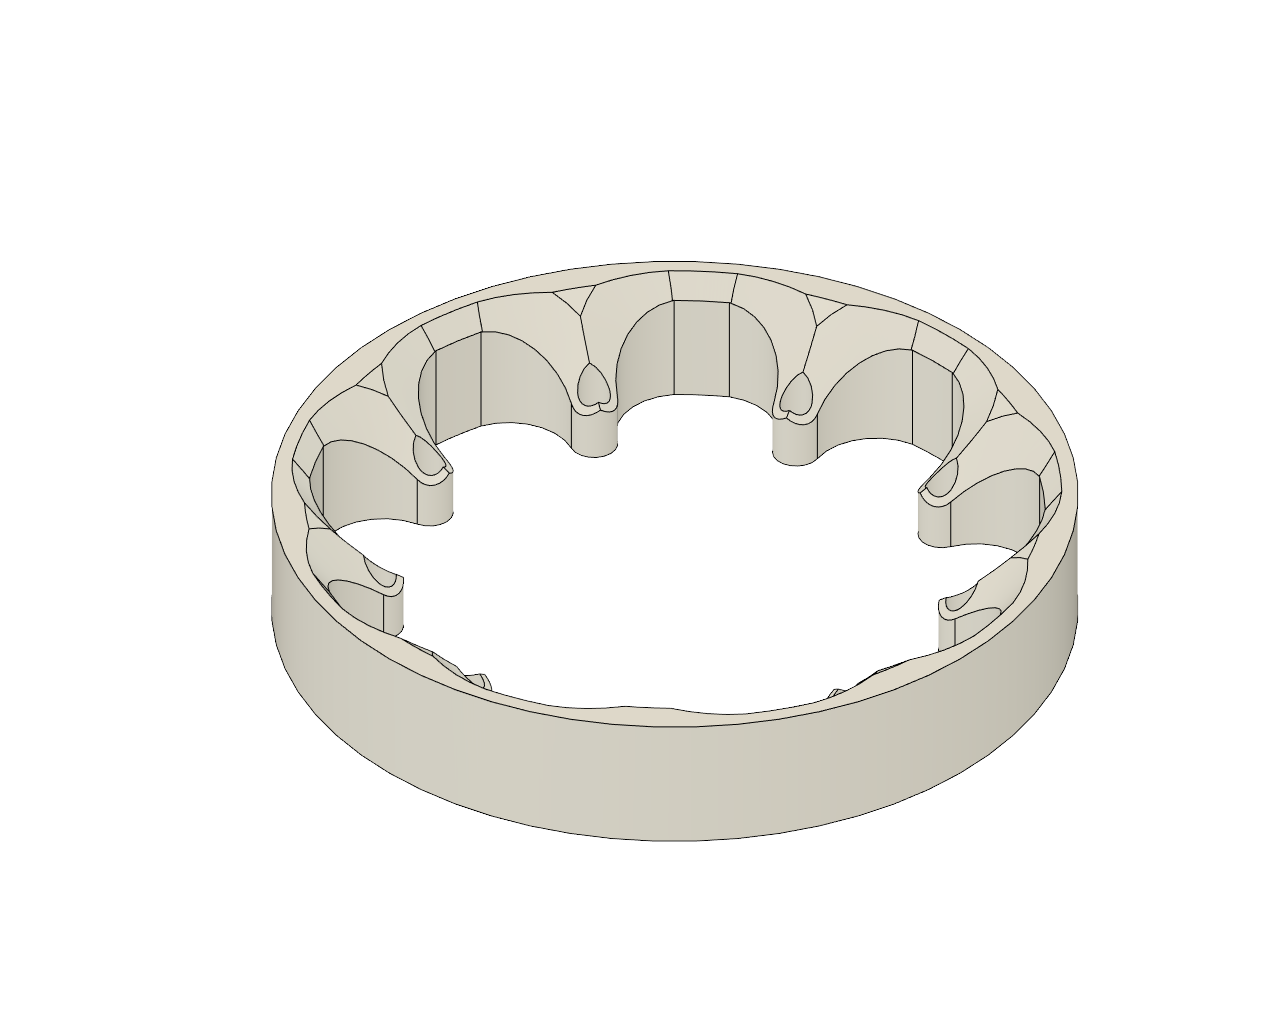
\includegraphics[width=0.7\columnwidth]{figure/设计方案/机械结构设计/22赛季中心供弹导流件.png}
        \end{minipage}
    }
    \subfigure[23赛季中心供弹导流件]{
        \begin{minipage}[t]{0.45\linewidth}
        \centering
        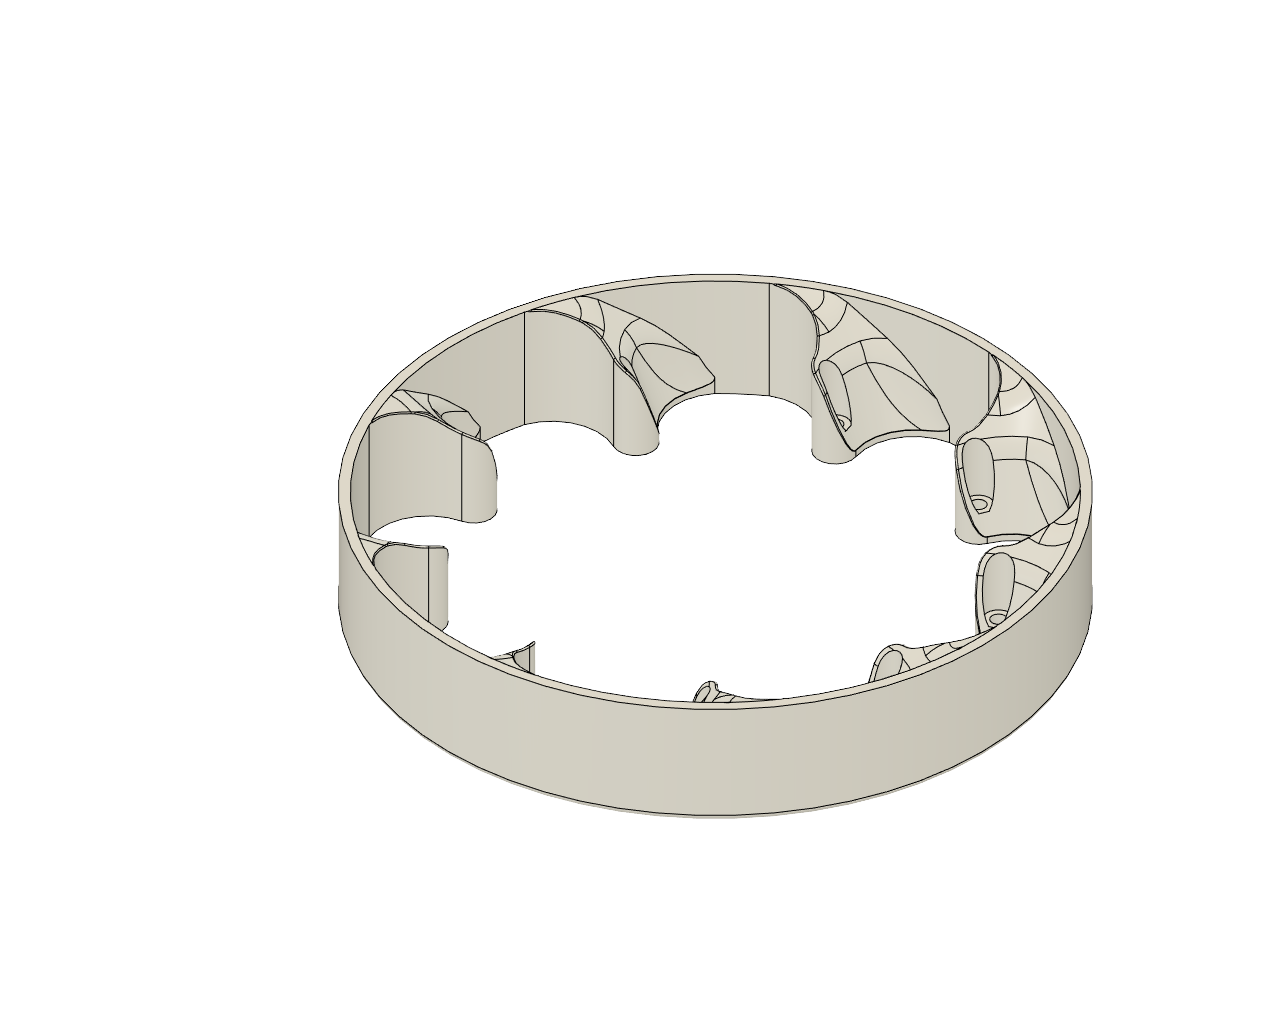
\includegraphics[width=0.7\columnwidth]{figure/设计方案/机械结构设计/23赛季中心供弹导流件.png}
        \end{minipage}
    }
    \caption{中心供弹导流件}
    \label{fig:中心供弹导流件}
\end{figure}

 \begin{figure}[hbt!]
    \centering
    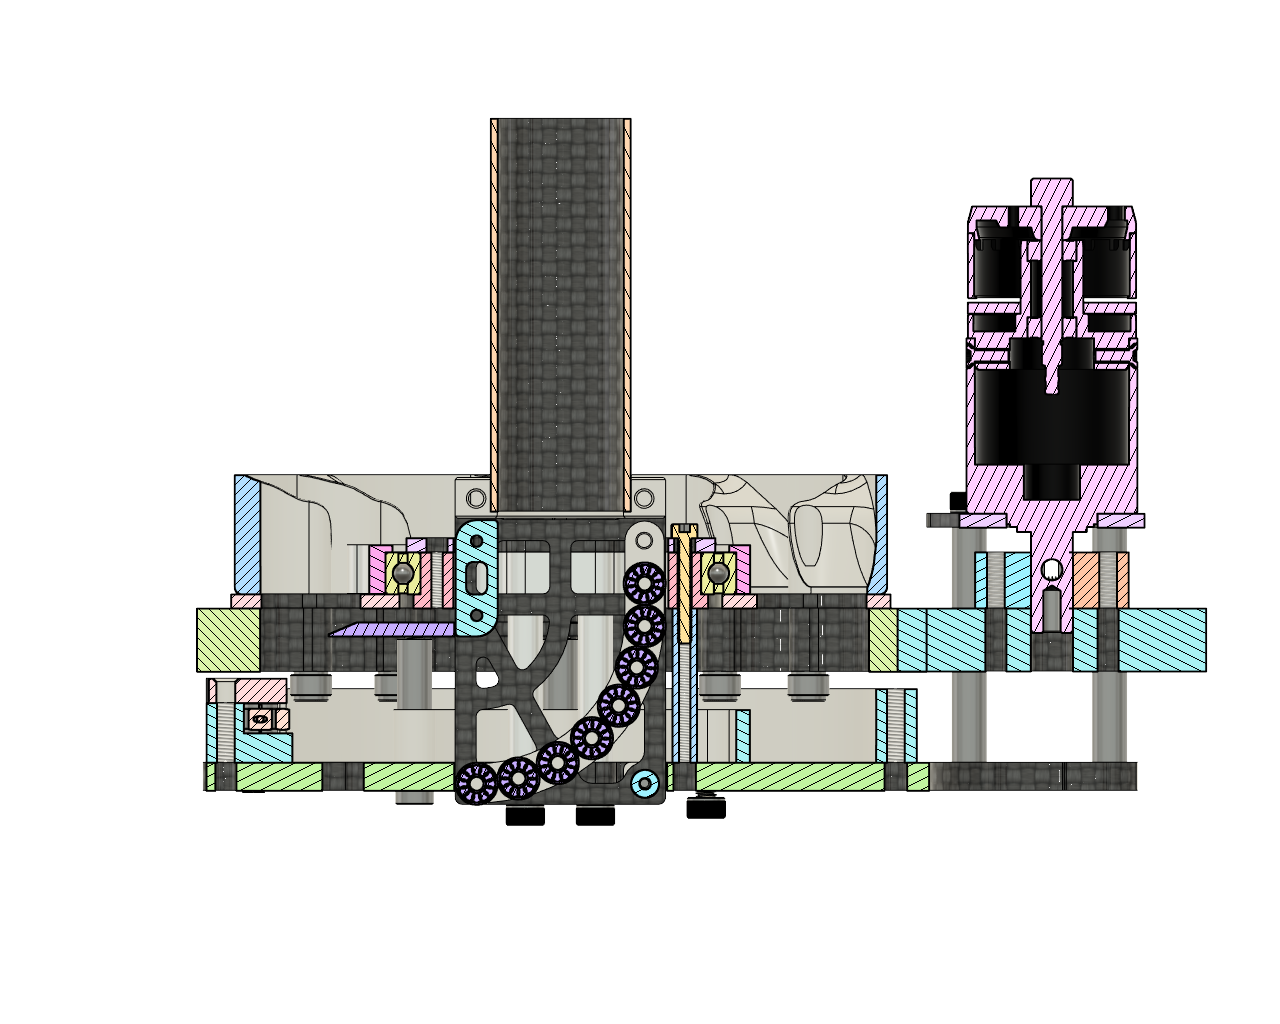
\includegraphics[width=0.5\columnwidth]{figure/设计方案/机械结构设计/中心供弹剖面图.png}
    \caption{中心供弹结构}
    \label{fig:中心供弹结构_设计方案}
\end{figure}

\paragraph{弹链结构}

链路使用2层$\qty{1}{\mm}$碳板和$1$层$\qty{2}{\mm}$碳板堆叠，利用$\qty{2}{\mm}$碳板垫高布置微型轴承减小链路阻力。该链路避免小的拐弯半径带来的推弹阻力，并保证Pitch轴在任何角度时弹丸相对摩擦轮的距离不会发生变化，避免误发射导致浪费弹丸。

\begin{figure}[hbt!]
    \centering
    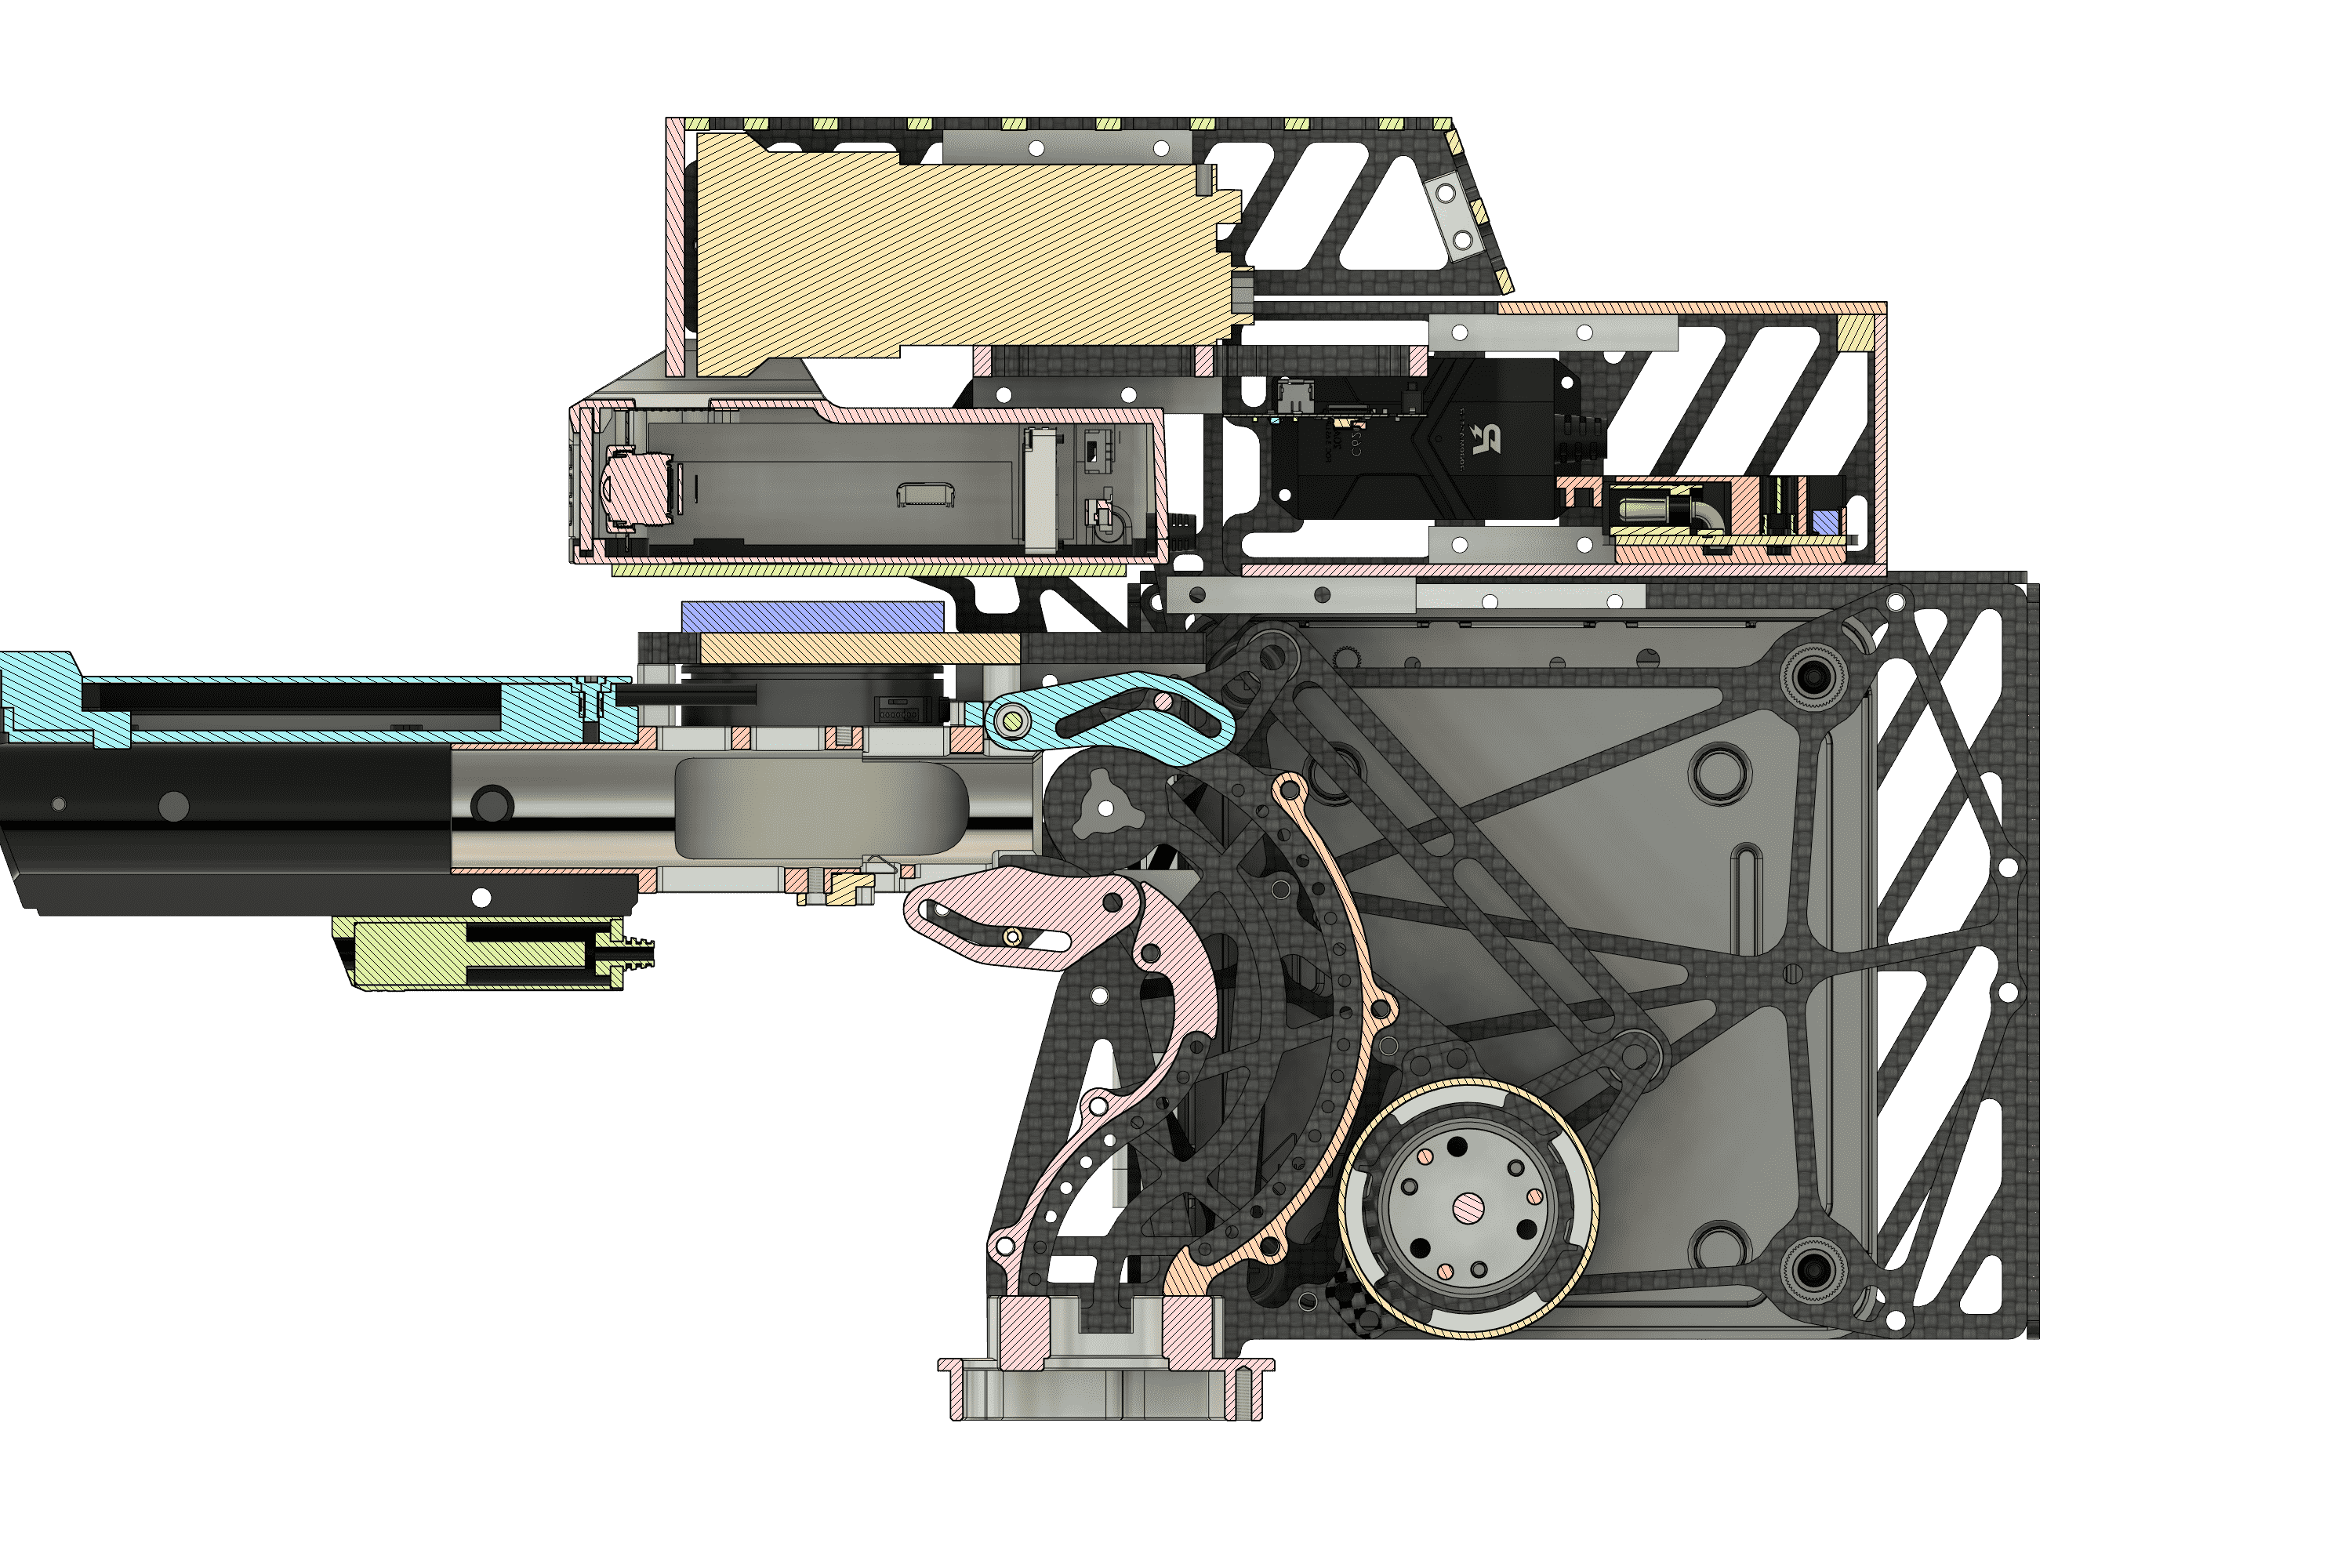
\includegraphics[width=0.5\columnwidth]{figure/设计方案/机械结构设计/云台弹链.png}
    \caption{云台弹链}
    \label{fig:云台弹链}
\end{figure}

弹链轴使用了上下两个活动滑槽，使发射机构在$\ang{30}$俯角$\sim$ $\ang{40}$仰角均可以流畅发弹，并且保证弹丸到摩擦轮的距离不会发生变化。弹链整体形状如\figref{fig:云台弹链}所示

\label{滑槽设计思路}滑槽设计通过在Pitch轴活动范围内均匀选取四个点，画出滑块会经过的点，同时不断调整活动滑槽的转轴和滑块的位置，来保证弹丸在滑槽中平稳运动，并且滑槽不会和云台结构干涉。在确定转轴位置和滑块经过的四个点后，将这四个点连线来拟合滑块的运动轨迹。最后在滑槽上添加圆角，避免滑块卡住。\figref{fig:P轴弹链滑块演示}展示了Pitch轴处于三种角度下的弹链滑块情况。

 \begin{figure}[hbt!]
    \centering
    \subfigure[P轴正50度]{
        \begin{minipage}[t]{0.3\linewidth}
        \centering
        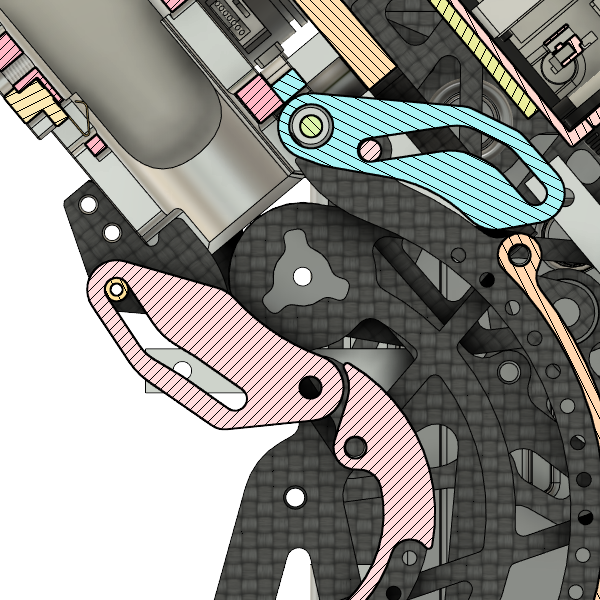
\includegraphics[width=0.7\columnwidth]{figure/设计方案/机械结构设计/P轴正50度.png}
        \end{minipage}
    }
    \subfigure[P轴水平]{
        \begin{minipage}[t]{0.3\linewidth}
        \centering
        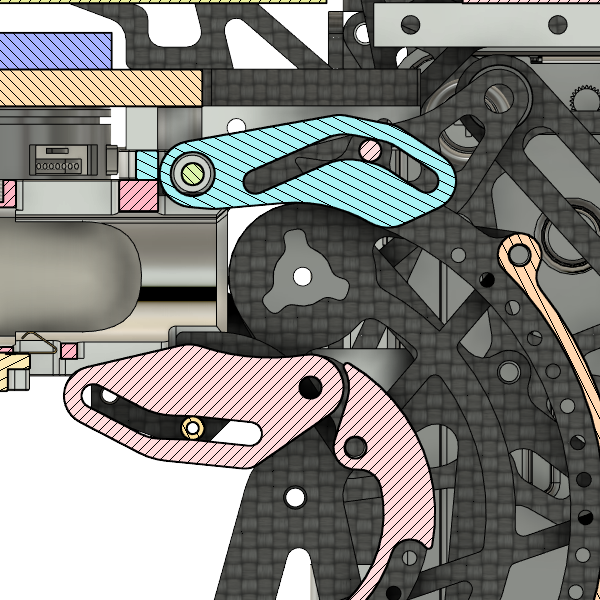
\includegraphics[width=0.7\columnwidth]{figure/设计方案/机械结构设计/P轴水平.png}
        \end{minipage}
    }
    \subfigure[P轴负30度]{
        \begin{minipage}[t]{0.3\linewidth}
        \centering
        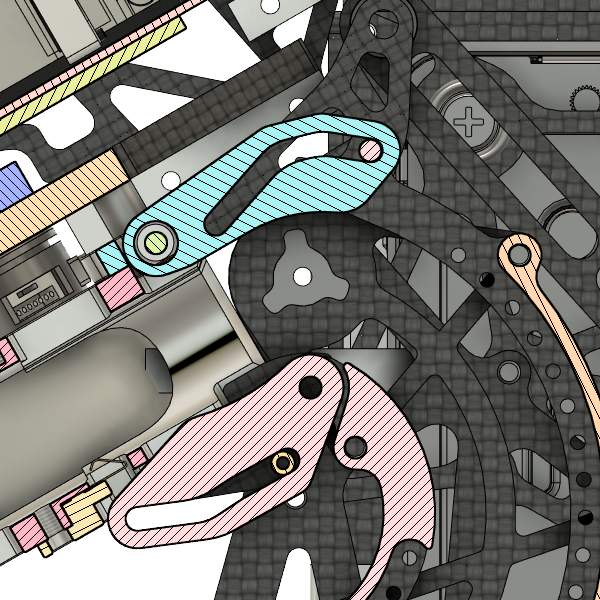
\includegraphics[width=0.7\columnwidth]{figure/设计方案/机械结构设计/P轴负30度.png}
        \end{minipage}
    }
    \caption{P轴弹链滑块演示}
    \label{fig:P轴弹链滑块演示}
\end{figure}

在23赛季哨兵发射机构测试的分析结果中(详见\ref{发射测试})，针对减小Pitch活动关节处弹链阻力这一方向，我们选择在上滑块及外部轴承保持架末端添加轴承的方案同时，由于原本的下滑块与23赛季新单发限位方案有冲突，我们微调了其形状，如\figref{fig:迭代弹链剖视图}所示。
\begin{figure}[hbt!]
    \centering
    \subfigure[22赛季弹链\label{fig:22赛季弹链} ]{
        \begin{minipage}[t]{0.45\linewidth}
        \centering
        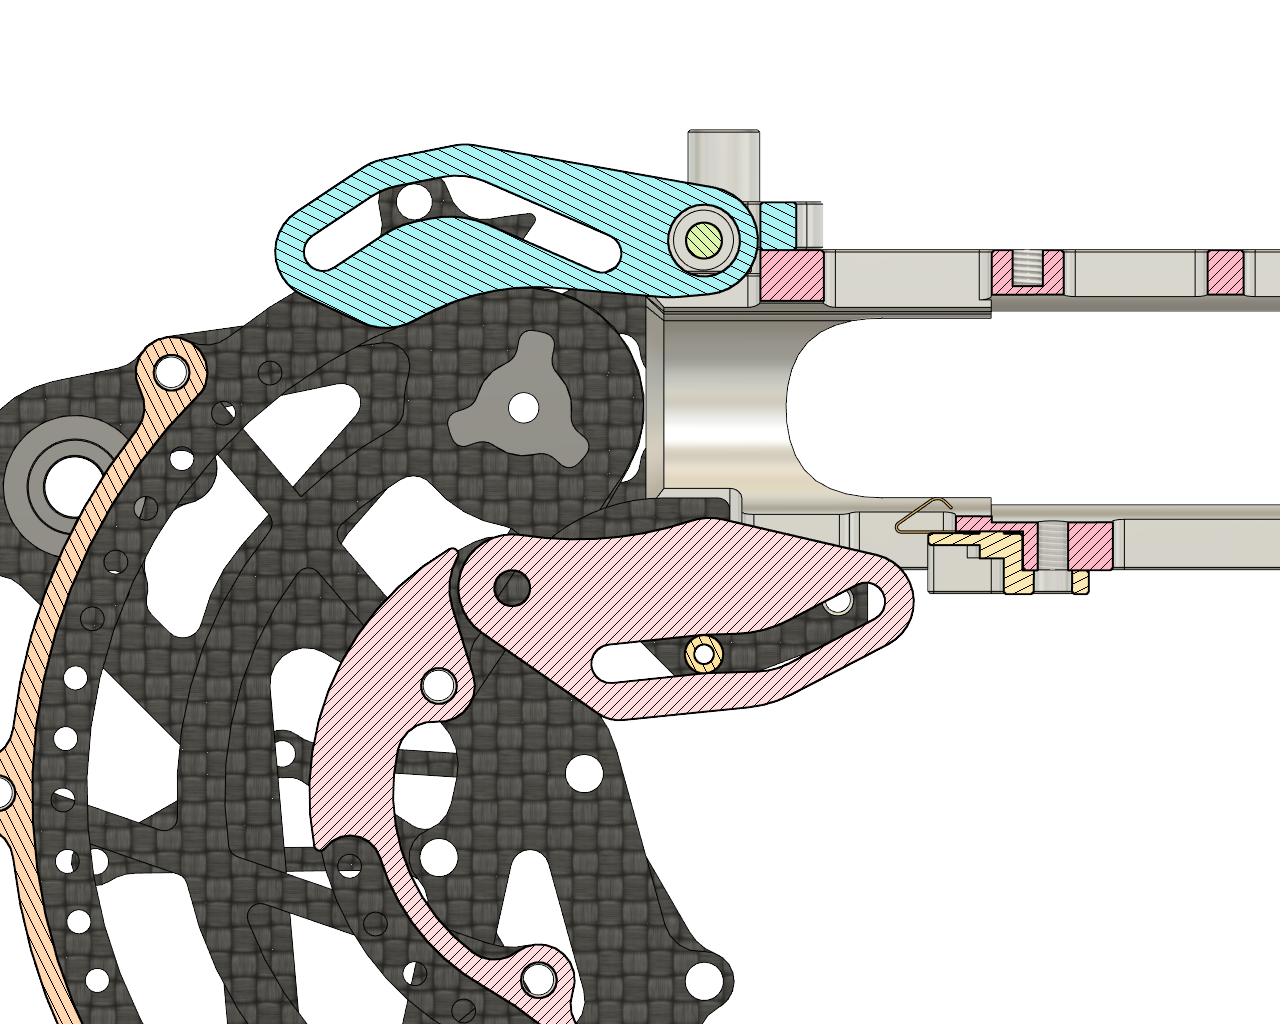
\includegraphics[width=0.7\columnwidth]{figure/设计方案/机械结构设计/22赛季弹链.png}
        \end{minipage}
    }
    \subfigure[23赛季弹链\label{fig:23赛季弹链}]{
        \begin{minipage}[t]{0.45\linewidth}
        \centering
        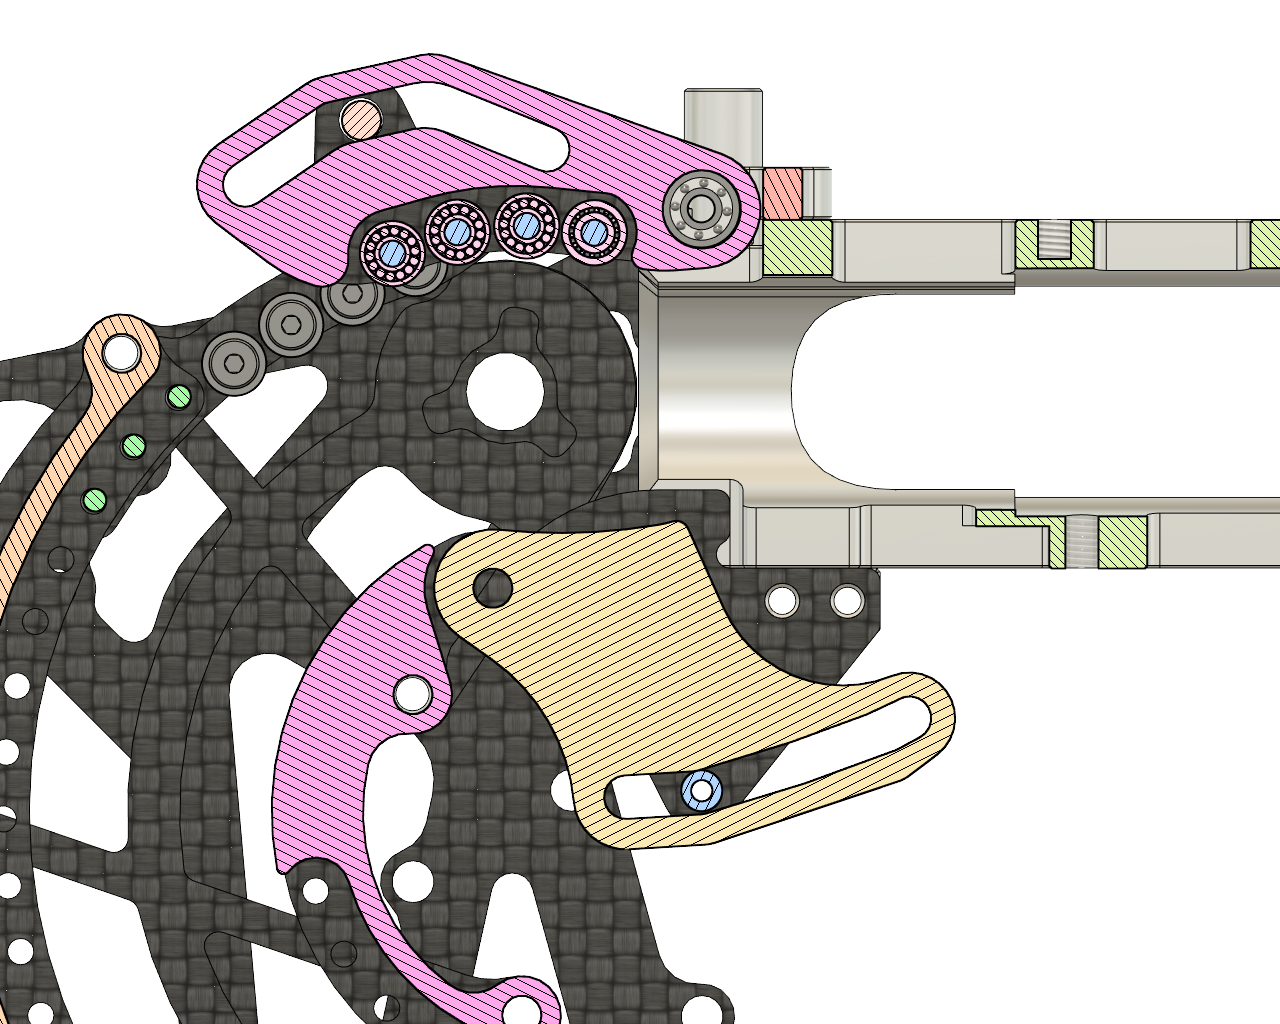
\includegraphics[width=0.7\columnwidth]{figure/设计方案/机械结构设计/23赛季弹链.png}
        \end{minipage}
    }

    \caption{弹链迭代剖视图}
    \label{fig:迭代弹链剖视图}
\end{figure}

在不改变上滑块内部轮廓的前提下，我们按照滑块设计理论(详见\ref{滑槽设计思路})，将上滑块的活动槽上移以留出轴承的空间，其爆炸图如\figref{fig:上滑块爆炸图}所示。这将使$\qty{17}{\mm}$弹丸与滑块在不同角度的摩擦从滑动摩擦变为滚动摩擦，有效降低其阻力。

\begin{figure}[hbt!]
    \centering
    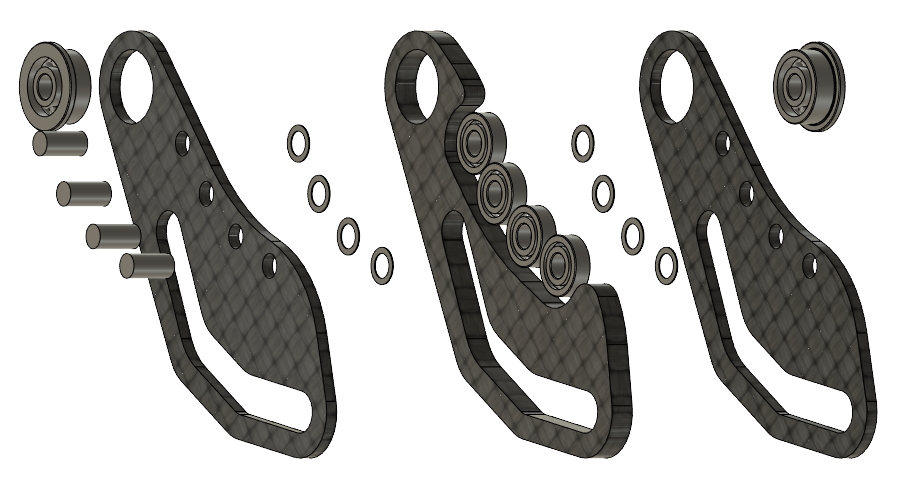
\includegraphics[width=0.5\columnwidth]{figure/设计方案/机械结构设计/上滑块爆炸图.png}
    \caption{上滑块爆炸图}
    \label{fig:上滑块爆炸图}
\end{figure}

\newpage

\subsection{工艺选择}
在哨兵机器人整体的设计过程中，综合机械制造的合理性，再结合本学校的加工设备资源、外包零件经费等情况，在哨兵机器人中采用了比较多的用2D雕刻加工玻纤板和碳纤板的结构设计（正常迭代使用玻纤板，最终比赛成车使用碳纤板），在一些必要的铝件上优化设计方案，设计出的铝件可以利用团队3轴铣床自加工，若出现复杂特征体的加工零部件，在经费充裕的情况下也可接受外包，结合3D打印件、部分弯管零部件、部分线切割的厚金属部件作辅助，部分工艺选择如\figref {fig:craft} 所示。

\begin{figure}[hbt!]
    \centering
    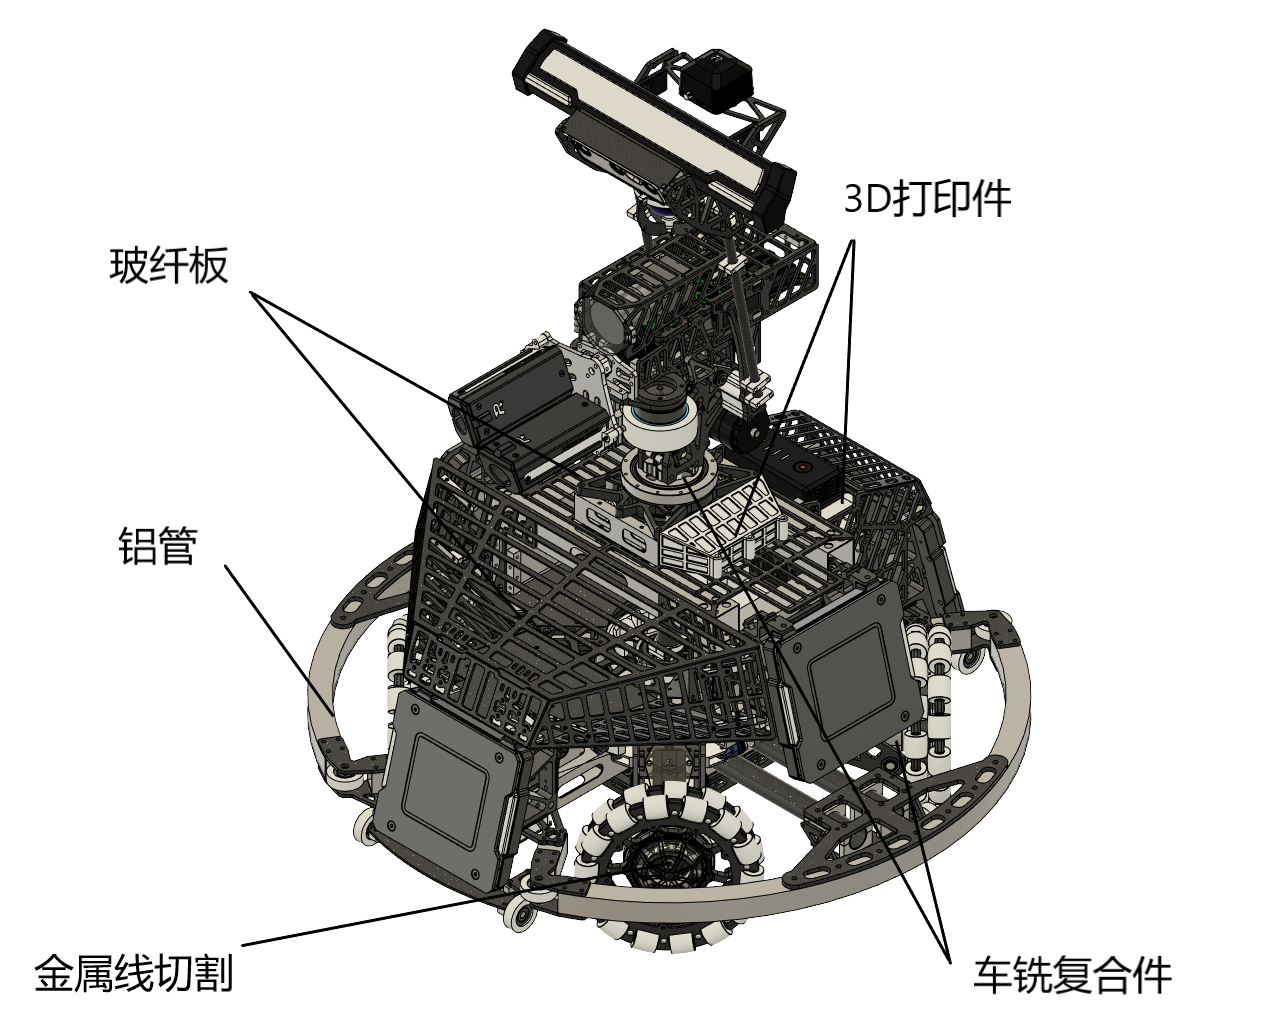
\includegraphics[width=0.6\columnwidth]{figure/设计方案/机械结构设计/哨兵总装轴测图.png}
    \caption{哨兵机器人工艺选择示意图}
    \label{fig:craft}
\end{figure}

\subsubsection{2D雕刻}
根据自己队伍的实际加工方式的情况，利用雕刻机可以可快速加工2D轮廓类的零部件，便于加快队伍在备赛期间的迭代速度，也可以节省迭代的成本，在结构设计上就尽可能使用板类零件，达到$80\%$可队内自我加工，尽量避免出现外包商的拖延而减缓进度的情况。加工如\figref {fig:2D}所展示。

\begin{figure}[!htbp]
    \centering
    \subfigure[铝管 \label{fig:2D_AL} ]{
        \begin{minipage}[t]{0.45\linewidth}
        \centering
        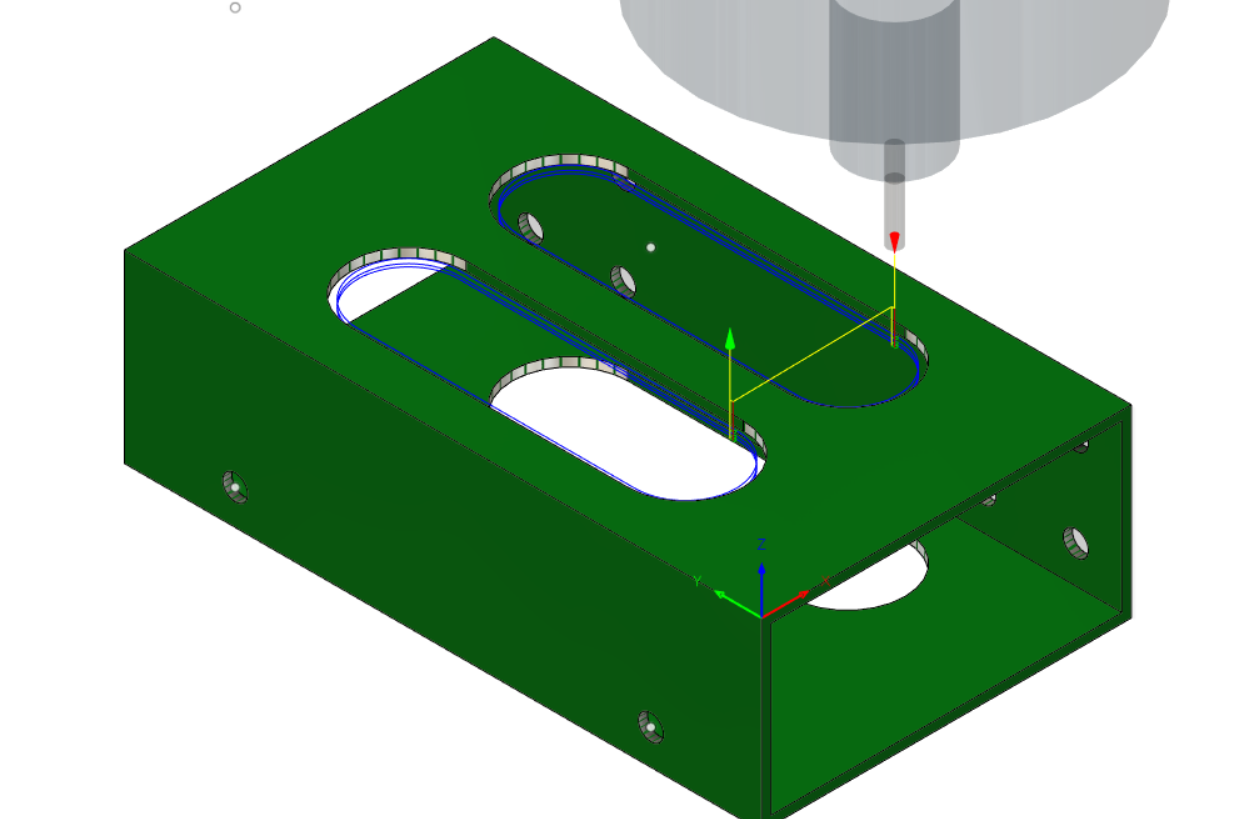
\includegraphics[width=0.6\columnwidth]{figure/设计方案/机械结构设计/path_Al.jpg}
        \end{minipage}
    }
    \subfigure[碳板\label{fig:2D_carbon}]{
        \begin{minipage}[t]{0.45\linewidth}
        \centering
        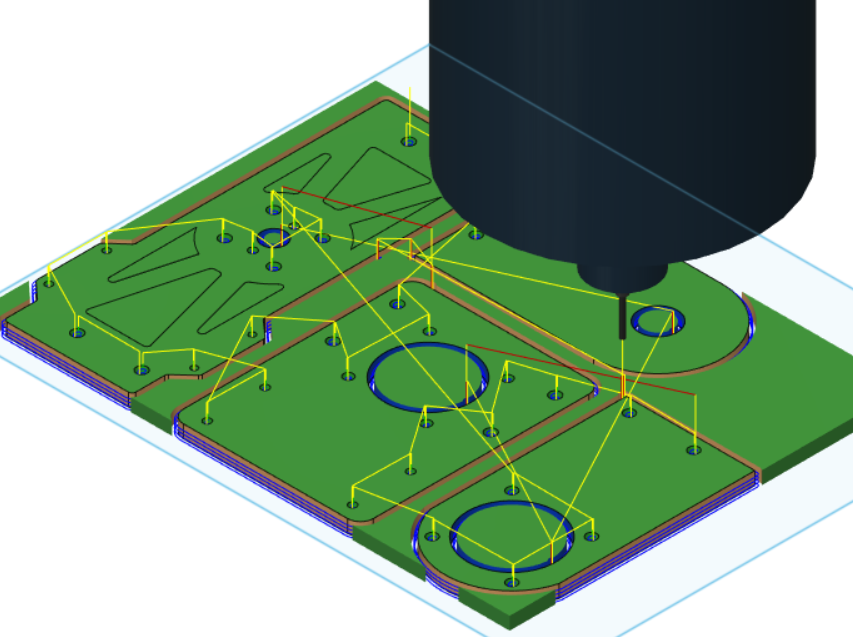
\includegraphics[width=0.6\columnwidth]{figure/设计方案/机械结构设计/path_Carbon plate.jpg}
        \end{minipage}
    }
    \caption{2D雕刻 \label{fig:2D}}
\end{figure}

\subsubsection{车铣复合加工}在整车设计过程中，不可避免的会出现一些因零部件的功能需求而导致外型复杂，或者是零件的尺寸精度要求高等情况，需要使用车铣复合加工，此时队内的加工设备已经无法制造，发外包商制造成了此类零部件的第一选择，比如发射的枪管铝件、轮毂电机的固定架、云台Yaw轴的固定铝件等。 如\figref {fig:mill}所展示。

\begin{figure}[!htbp]
    \centering
    \subfigure[云台铝件 \label{fig:Gimbal_aluminum_parts} ]{
        \begin{minipage}[t]{0.45\linewidth}
        \centering
        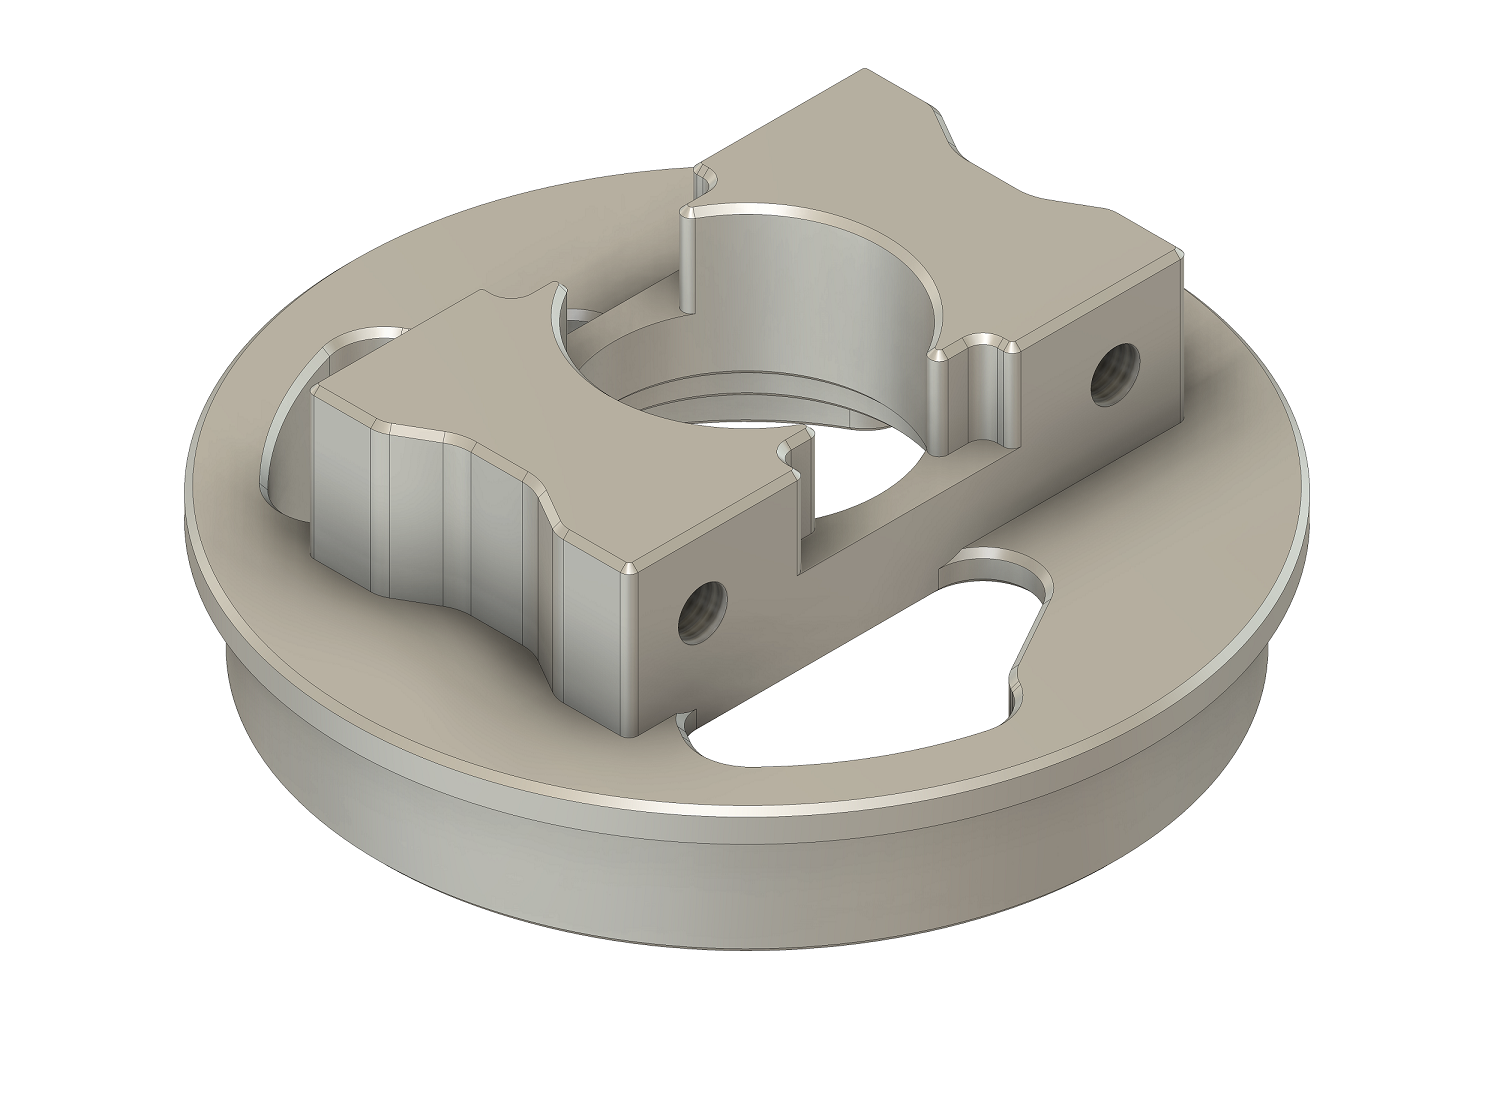
\includegraphics[width=0.6\columnwidth]{figure/设计方案/机械结构设计/云台铝件.png}
        \end{minipage}
    }
    \subfigure[轮毂电机铝件\label{fig:Hub_motor}]{
        \begin{minipage}[t]{0.45\linewidth}
        \centering
        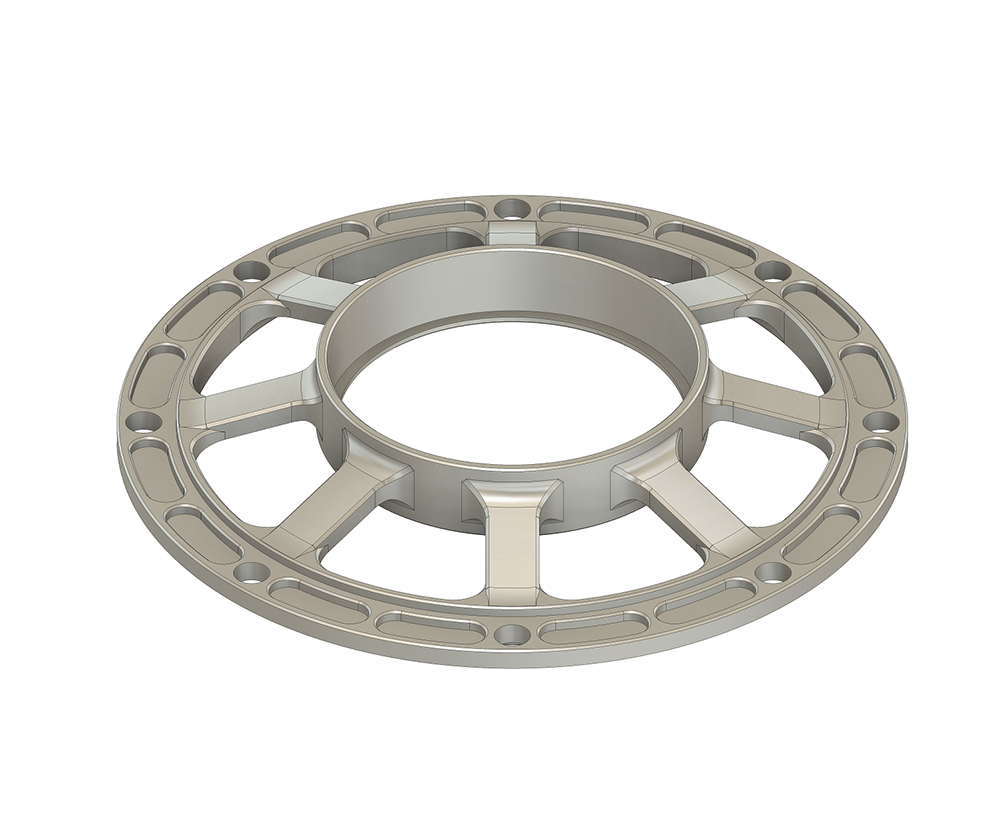
\includegraphics[width=0.6\columnwidth]{figure/设计方案/机械结构设计/轮毂电机铝件.jpg}
        \end{minipage}
    }
    \caption{车铣复合加工 \label{fig:mill}}
\end{figure}

\subsubsection{3D打印}
3D打印作为非规则模型的加工非常便利，面对着一些拥有曲面的、强度要求不高、作平常固定非支撑件的零件，首选均为3D打印。 如\figref {fig:3D_print}所展示。

\begin{figure}[!htbp]
    \centering
    \subfigure[防尘盖 \label{fig:3D_dustproof} ]{
        \begin{minipage}[t]{0.45\linewidth}
        \centering
        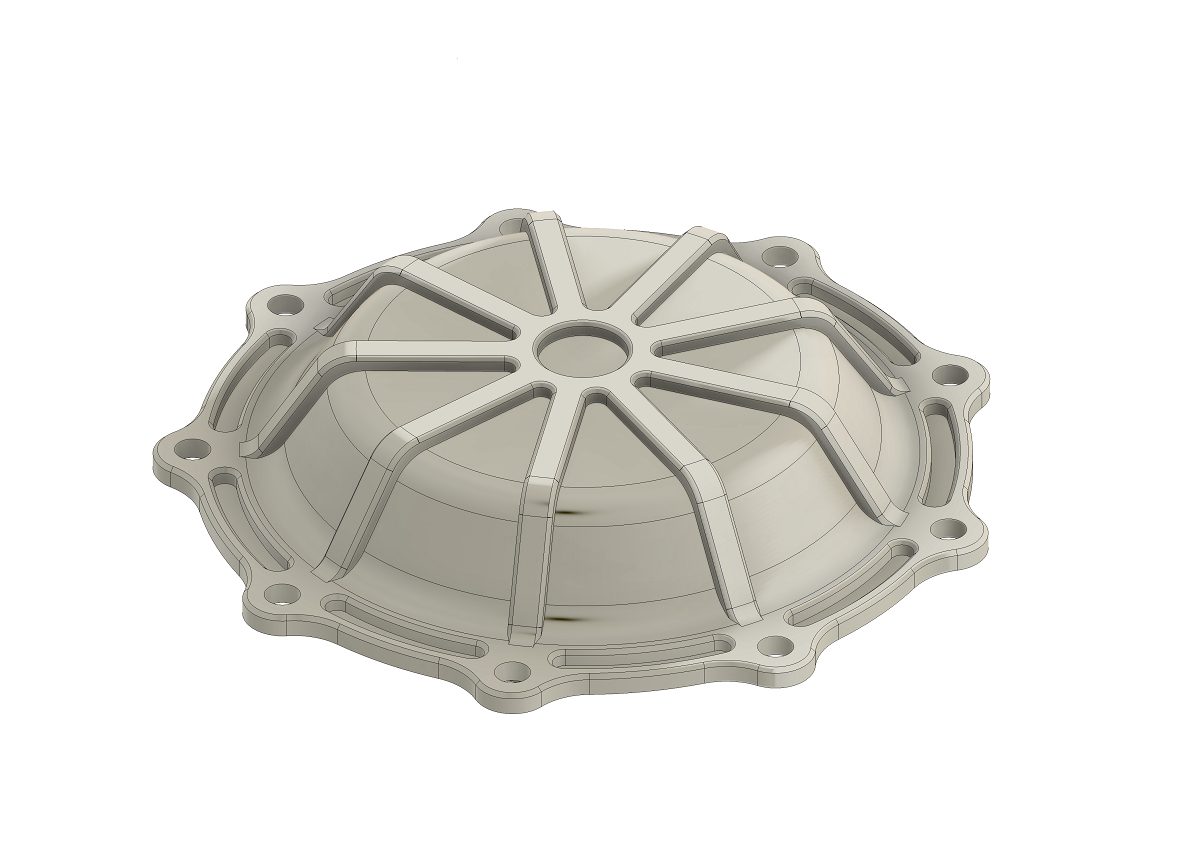
\includegraphics[width=0.6\columnwidth]{figure/设计方案/机械结构设计/防尘盖.png}
        \end{minipage}
    }
    \subfigure[滑环外壳\label{fig:3D_enclosure}]{
        \begin{minipage}[t]{0.45\linewidth}
        \centering
        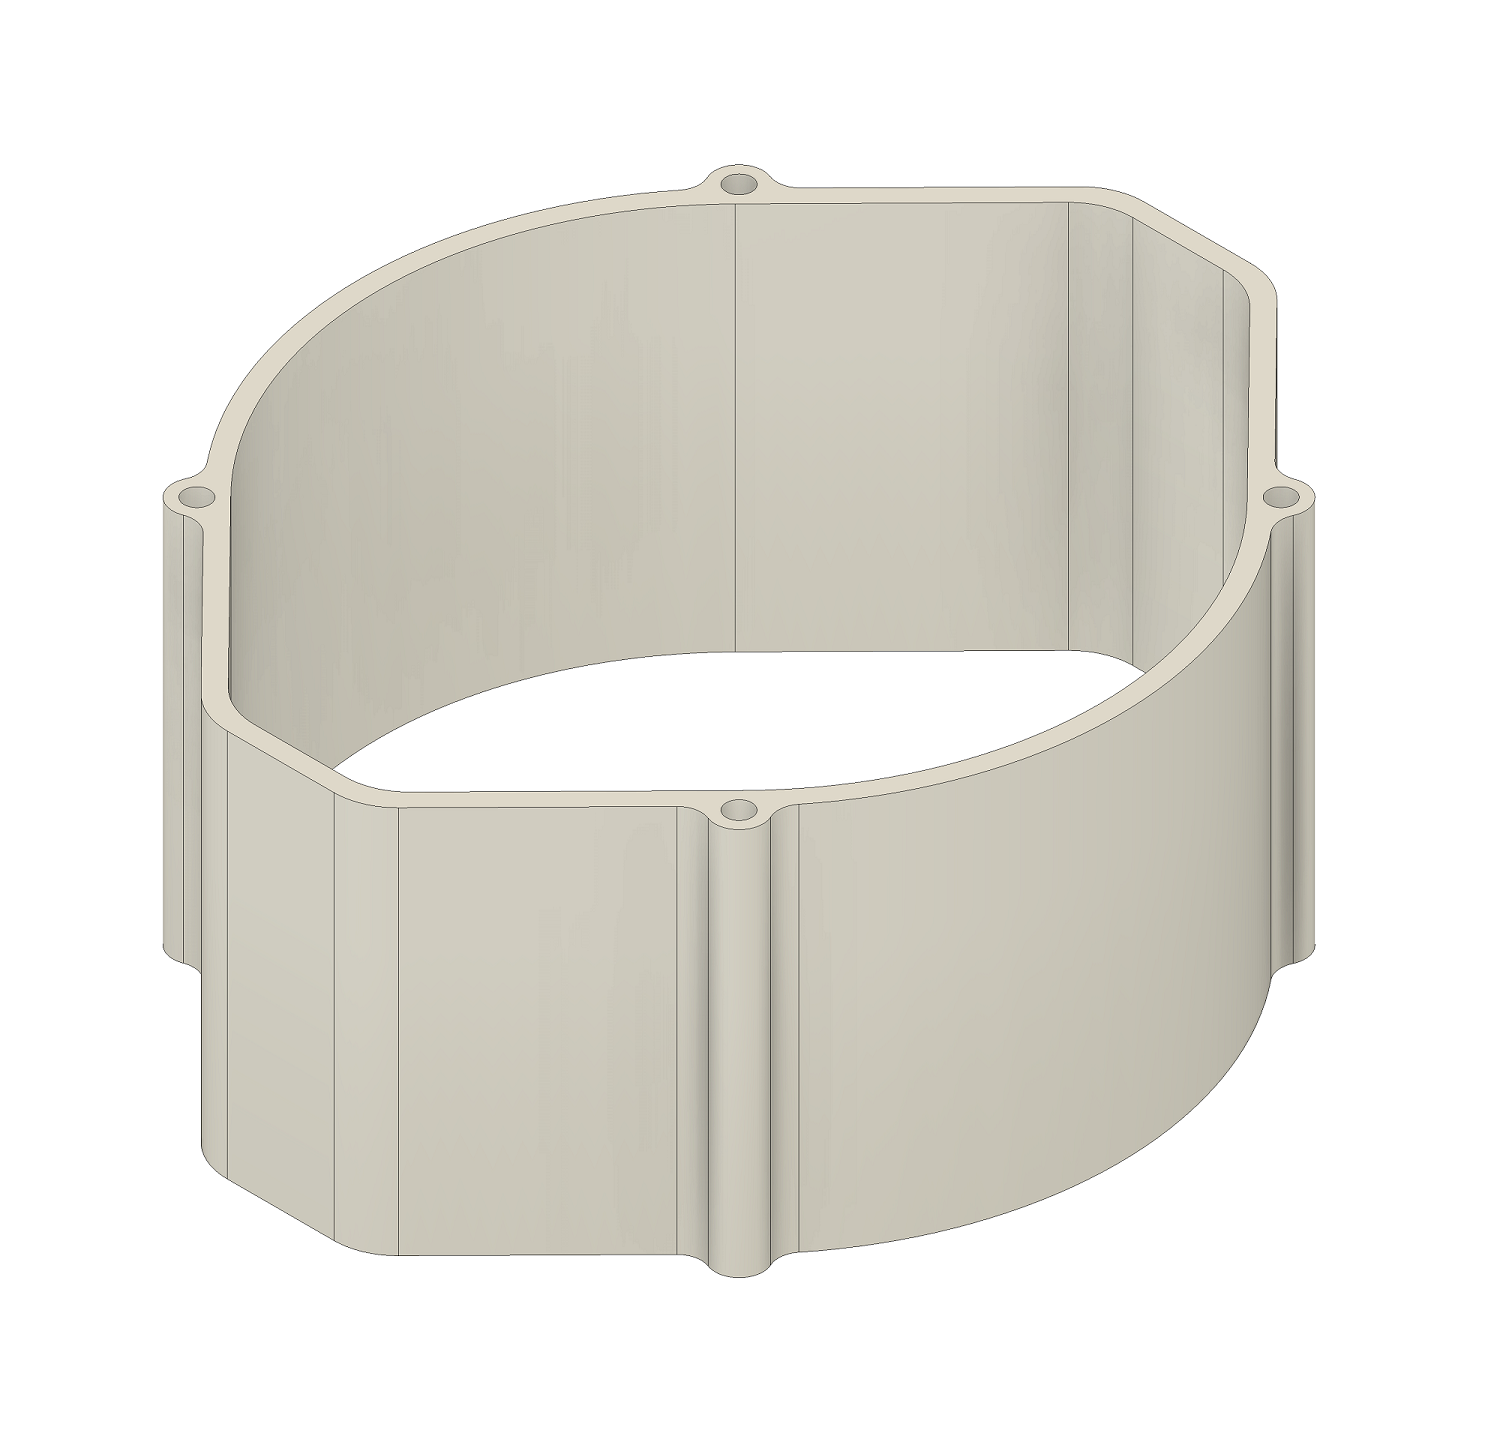
\includegraphics[width=0.4\columnwidth]{figure/设计方案/机械结构设计/滑环外壳.png}
        \end{minipage}
    }
    \caption{3D打印 \label{fig:3D_print}}
\end{figure}

\subsubsection{线切割}
对于厚度大的零部件，如自制减速器中的齿轮和齿圈，材料为模具钢，此时使用外包线切割加工更为合适。如\figref {fig:Wire_cutting}所展示。

\begin{figure}[!htbp]
    \centering
    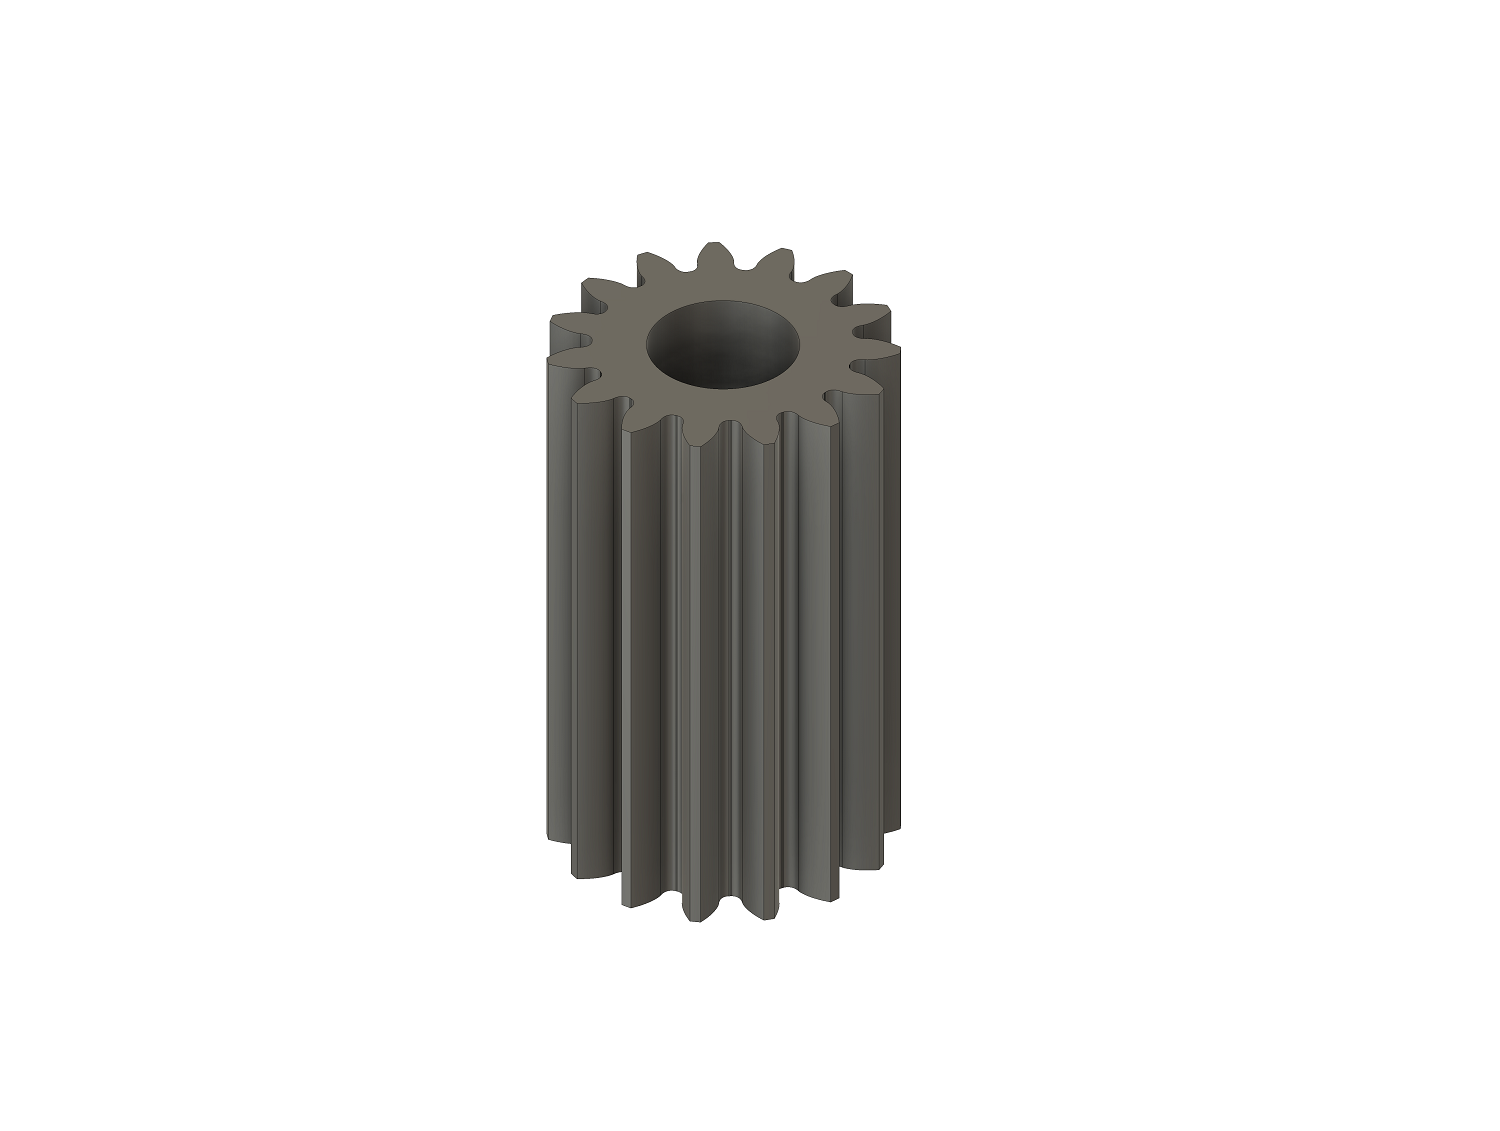
\includegraphics[width=0.3\columnwidth]{figure/设计方案/机械结构设计/线切割齿轮.png}
        \caption{线切割齿轮}
        \label{fig:Wire_cutting}
\end{figure}

\subsubsection{弯管}
由于哨兵机器人的自旋速度较快，并且在比赛场地激烈交战的通道一般比较狭窄，极易碰撞到其他机器人或者场地边缘，故外保护框设计成圆形，可以有效避免碰撞的自旋速度损耗，材料选择为铝管，利用手动弯管机加工成型。如\figref {fig:curved}所示。

\begin{figure}[hbt!]
    \centering
    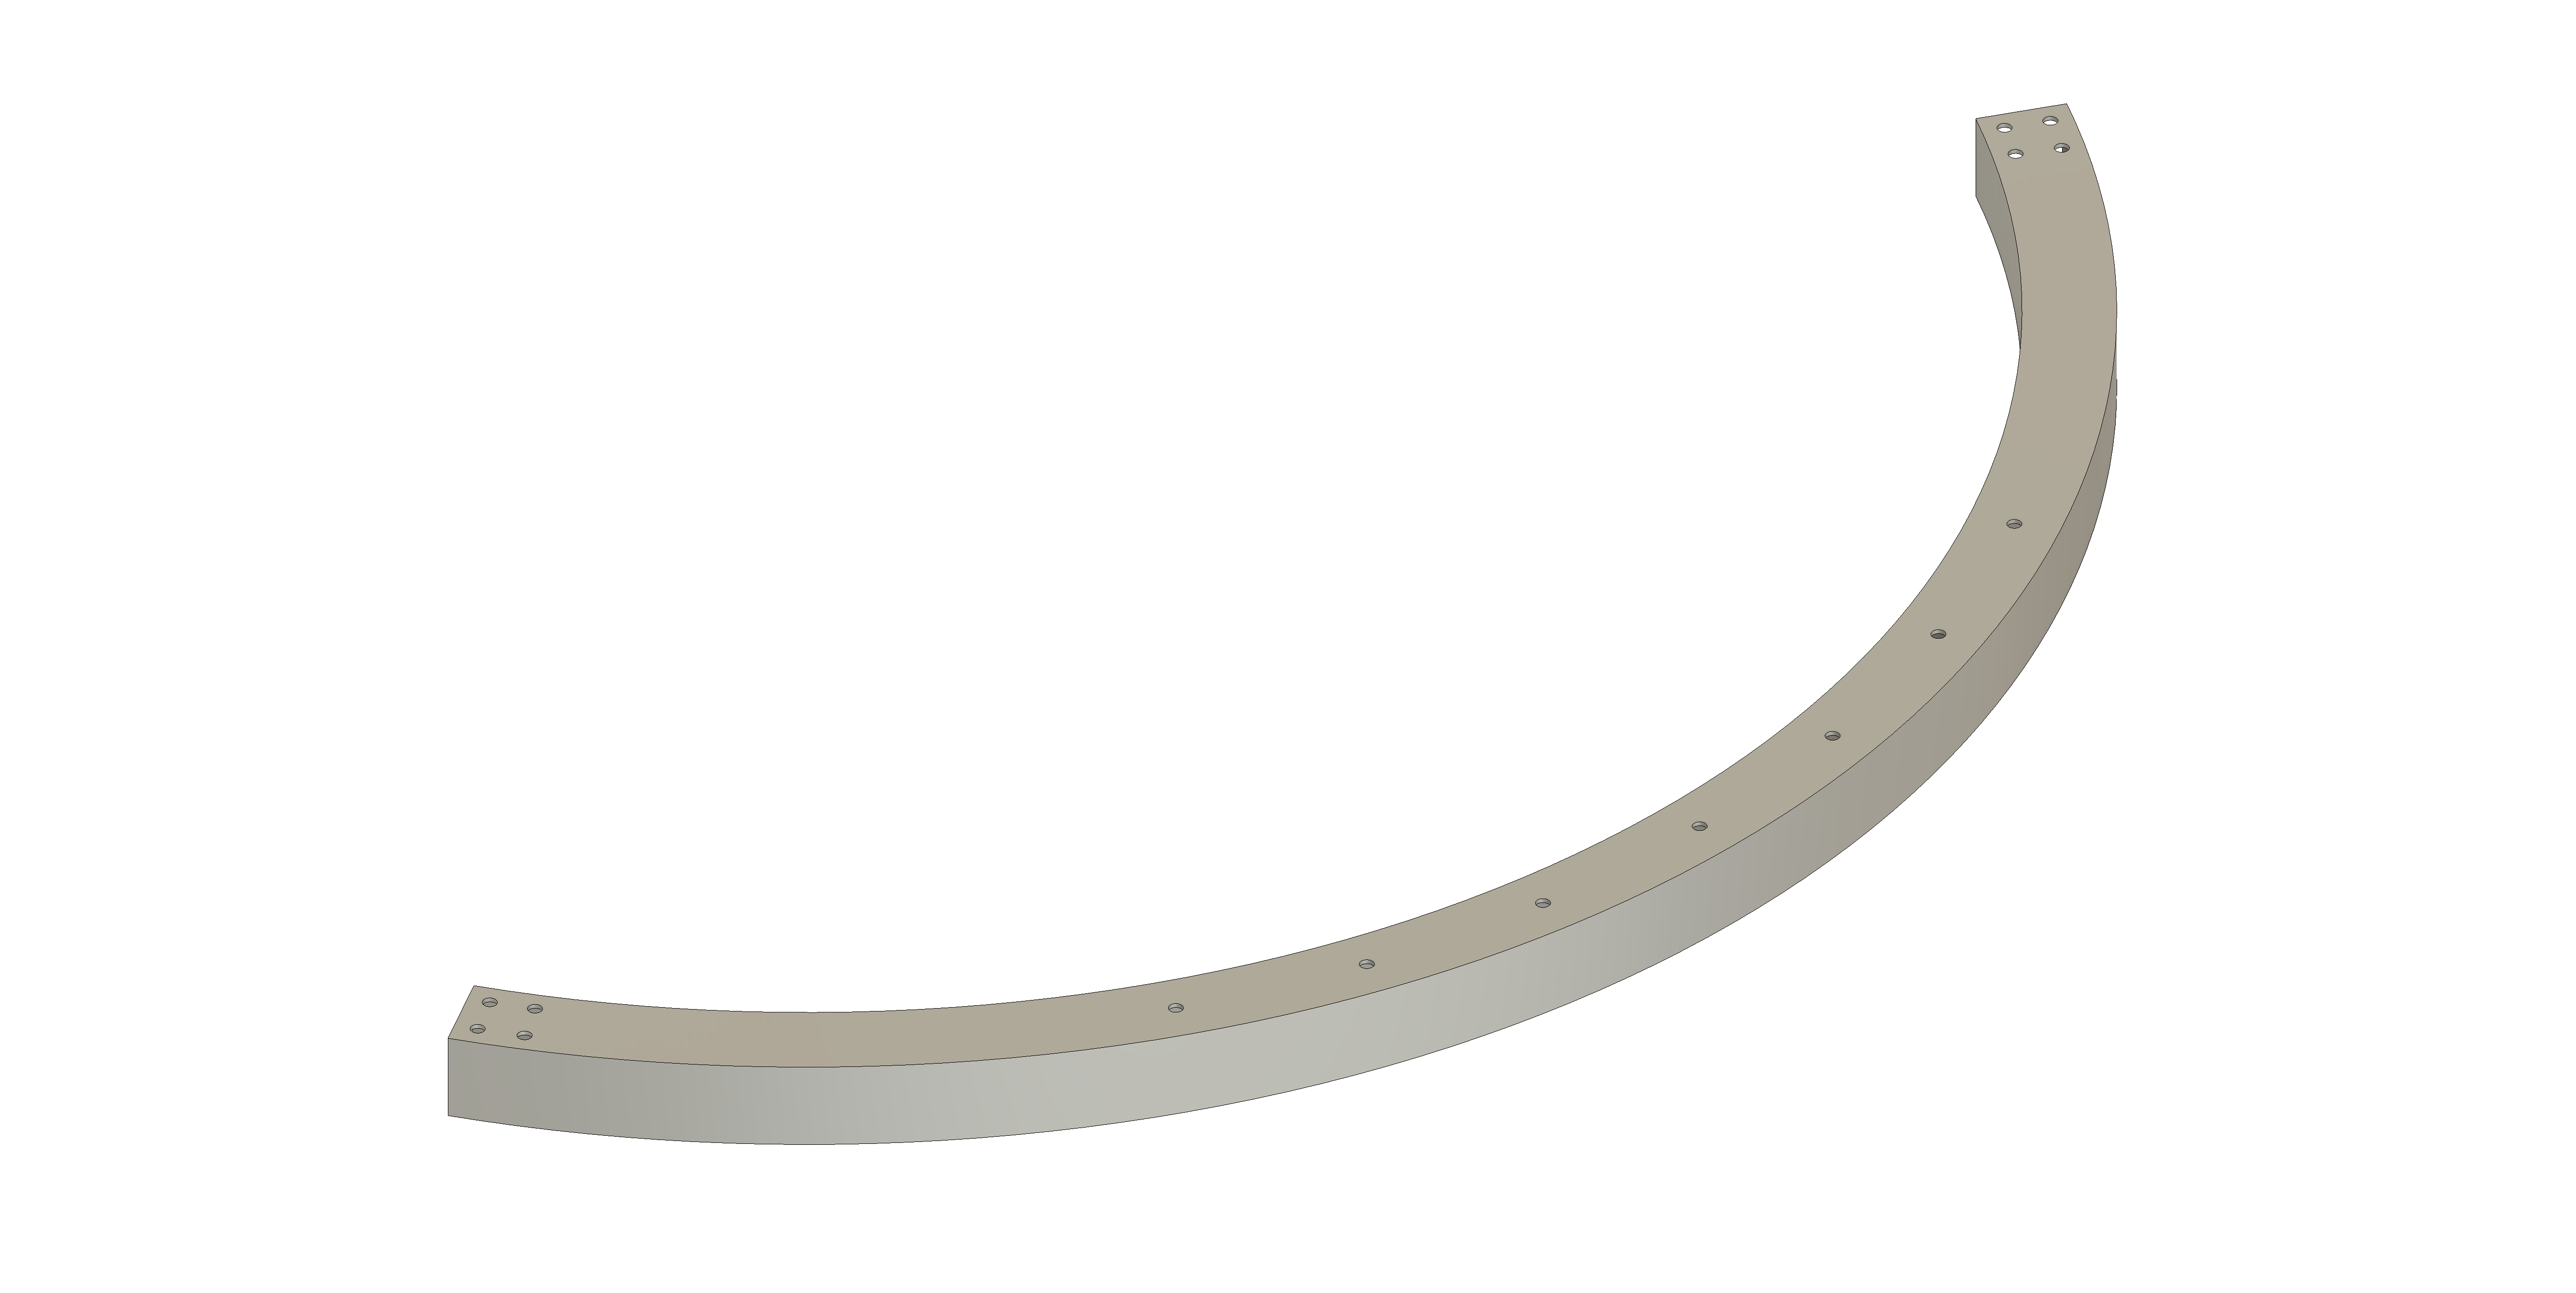
\includegraphics[width=0.4\columnwidth]{figure/设计方案/机械结构设计/保护框.png}
    \caption{保护框弯管}
    \label{fig:curved}
\end{figure}

\subsection{传感器的设计安装、电路板的固定及连接} 
机器人各个传感器与电路板都采用螺丝连接的方式，与板件刚性连接，在需要绝缘的地方使用绝缘材质连接，既保证各个传感器与电路板的正常工作，同时也保证各个硬件与机器人的固定。

如 \figref {fig:IMU_设计方案}所展示，惯性测量单元IMU由四颗螺丝固定在四根带螺纹的尼龙柱上，再通过螺丝连接的方式将尼龙柱与一块高刚性的板件连接，通过这种方式，使IMU固定在一块高刚性的板件的下端。摄像头通过螺丝连接在IMU固定板件上端，使摄像头与IMU可以作为一个整体的模块在云台上安装与拆卸，避免控制组需要频繁地对IMU和相机进行联合标定。尼龙柱在此处不仅起到IMU的固定作用，保证IMU与板件的刚性连接，同时也可以起到绝缘作用，防止金属与IMU直接接触而导致短路损坏IMU。
\begin{figure}[hbt!]
    \centering
    \subfigure[IMU固定侧视图 \label{fig:IMU1_设计方案} ]{
        \begin{minipage}[t]{0.45\linewidth}
        \centering
        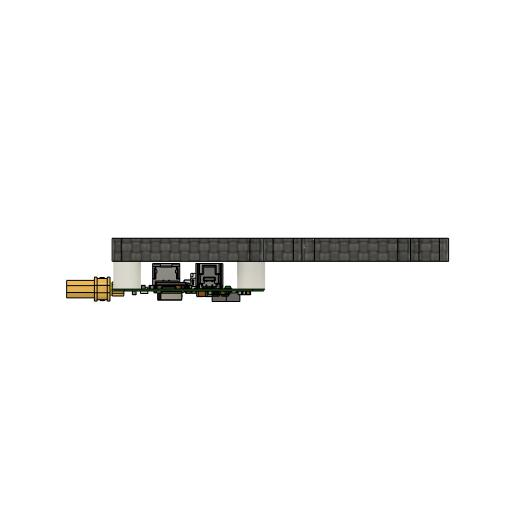
\includegraphics[width=0.7\columnwidth]{figure/设计方案/机械结构设计/IMU固定侧视图.jpg}
        \end{minipage}
    }
    \subfigure[IMU固定俯视图\label{fig:IMU2_设计方案}]{
        \begin{minipage}[t]{0.45\linewidth}
        \centering
        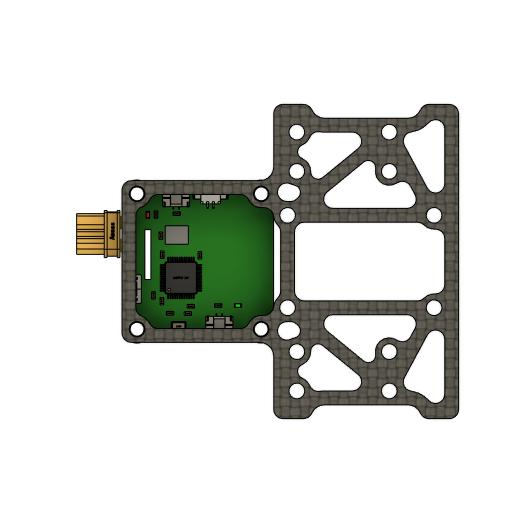
\includegraphics[width=0.7\columnwidth]{figure/设计方案/机械结构设计/IMU固定俯视图.jpg}
        \end{minipage}
    }
    \caption{IMU固定展示 \label{fig:IMU_设计方案}}
\end{figure} 

如 \figref {fig:摄像头_设计方案}
所展示，摄像头通过四根螺丝与摄像头固定板刚性连接，保证摄像头在机器人运动过程中的连接稳定性。摄像头四周通过$\qty{2}{\mm}$板件围成摄像头保护壳，板件通过板板连接件连接，以保证摄像头保护壳的坚固性，确保在比赛过程中对摄像头的稳定保护。在摄像头前端装有一块$\qty{3}{\mm}$亚克力板，既保证了对摄像头镜头的保护，同时不会遮挡摄像头的视角。

\begin{figure}[hbt!]
    \centering
    \subfigure[摄像头固定侧视图 \label{fig:摄像头1_设计方案} ]{
        \begin{minipage}[t]{0.45\linewidth}
        \centering
        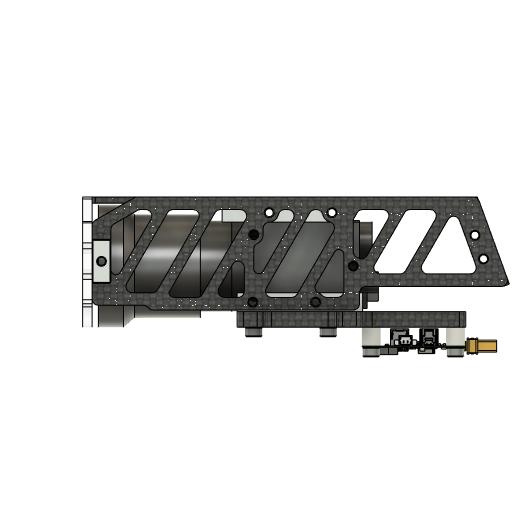
\includegraphics[width=0.7\columnwidth]{figure/设计方案/机械结构设计/摄像头固定侧视图.jpg}
        \end{minipage}
    }
    \subfigure[摄像头固定仰视图\label{fig:摄像头2_设计方案}]{
        \begin{minipage}[t]{0.45\linewidth}
        \centering
        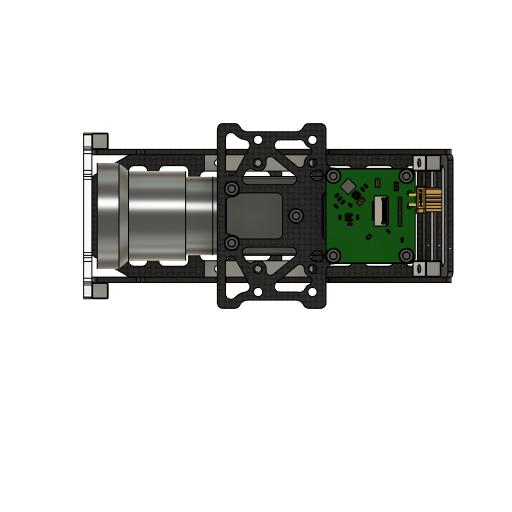
\includegraphics[width=0.7\columnwidth]{figure/设计方案/机械结构设计/摄像头固定仰视图.jpg}
        \end{minipage}
    }
    \caption{摄像头固定展示 \label{fig:摄像头_设计方案}}
\end{figure} 

如 \figref {fig:雷达_设计方案}
所展示，雷达通过四根螺丝与雷达固定板刚性连接，保证雷达机器人运动过程中的连接稳定性。雷达四周通过$\qty{2}{\mm}$板件围成雷达保护壳，板件通过板板连接件以及打印件连接，以保证雷达保护壳的坚固性，确保在比赛过程中对雷达的稳定保护。在雷达上端装有$\qty{2}{\mm}$的十字保护罩，既保证了对雷达的保护，同时不会造成过多遮挡。

如 \figref {fig:大恒相机_设计方案}
所展示，大恒相机通过四根螺丝与相机固定板刚性连接，保证相机在机器人运动过程中的连接稳定性。相机四周通过$\qty{2}{\mm}—\qty{4}{\mm}$板件围成摄像头保护壳，板件通过板板连接件连接，以保证相机保护壳的坚固性，确保在比赛过程中对摄像头的稳定保护。在摄像头前端装有一块$\qty{2}{\mm}$亚克力板，既保证了对摄像头镜头的保护，同时不会遮挡摄像头的视角。

\begin{figure}[hbt!]
    \centering
    \subfigure[雷达保护及固定 斜二测 \label{fig:雷达1_设计方案} ]{
        \begin{minipage}[t]{0.45\linewidth}
        \centering
        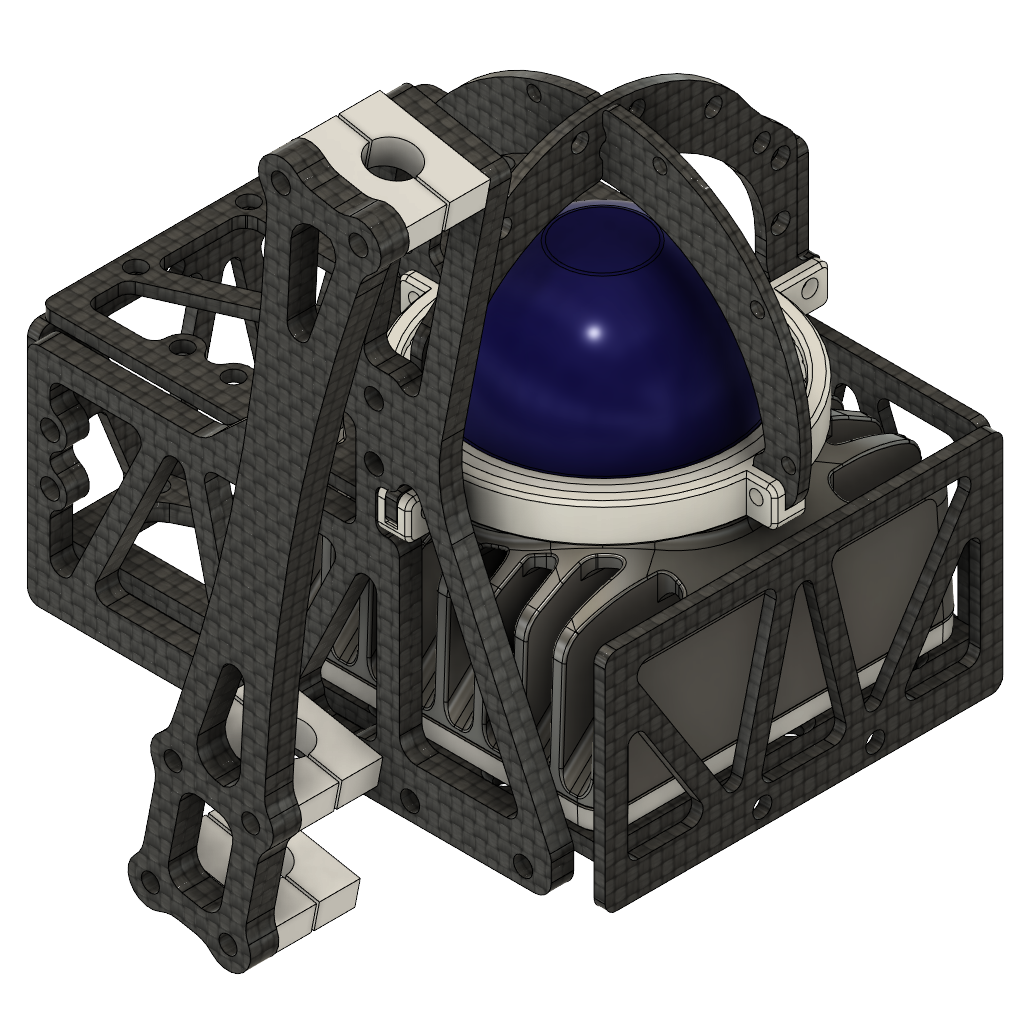
\includegraphics[width=0.6\columnwidth]{figure/设计方案/机械结构设计/雷达保护及固定 斜二测.png}
        \end{minipage}
    }
    \subfigure[雷达固定仰视图\label{fig雷达2_设计方案}]{
        \begin{minipage}[t]{0.45\linewidth}
        \centering
        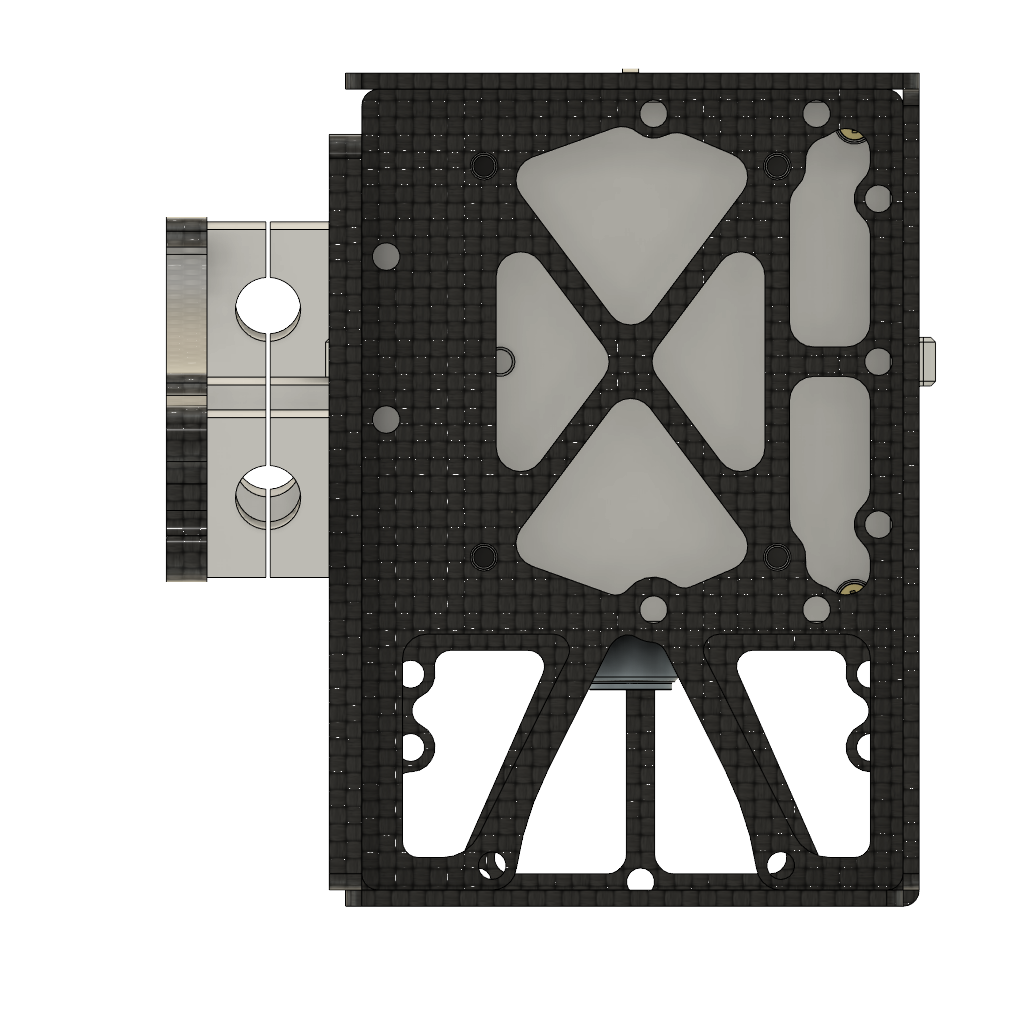
\includegraphics[width=0.6\columnwidth]{figure/设计方案/机械结构设计/雷达固定 仰视图.png}
        \end{minipage}
    }
    \caption{雷达固定展示 \label{fig:雷达_设计方案}}
\end{figure} 


\begin{figure}[hbt!]
    \centering
    \subfigure[大恒相机固定及保护\label{fig:大恒相机1_设计方案} ]{
        \begin{minipage}[t]{0.45\linewidth}
        \centering
        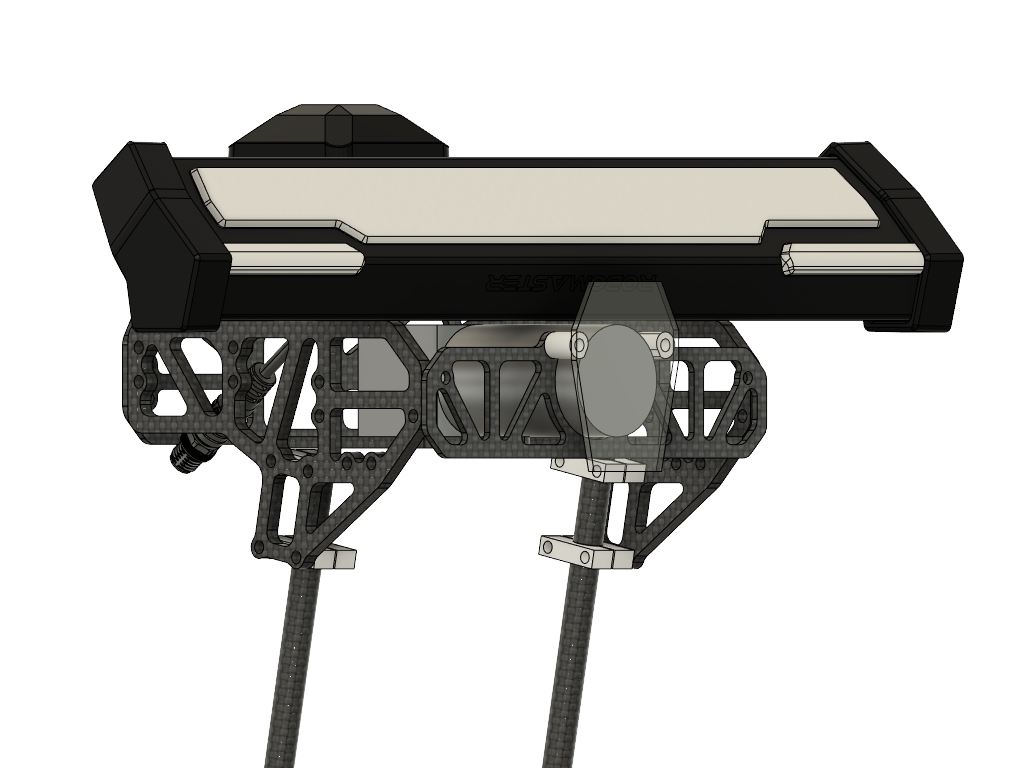
\includegraphics[width=0.6\columnwidth]{figure/设计方案/机械结构设计/大恒相机固定及保护.png}
        \end{minipage}
    }
    \subfigure[大恒相机固定仰视图\label{fig:大恒相机2_设计方案}]{
        \begin{minipage}[t]{0.45\linewidth}
        \centering
        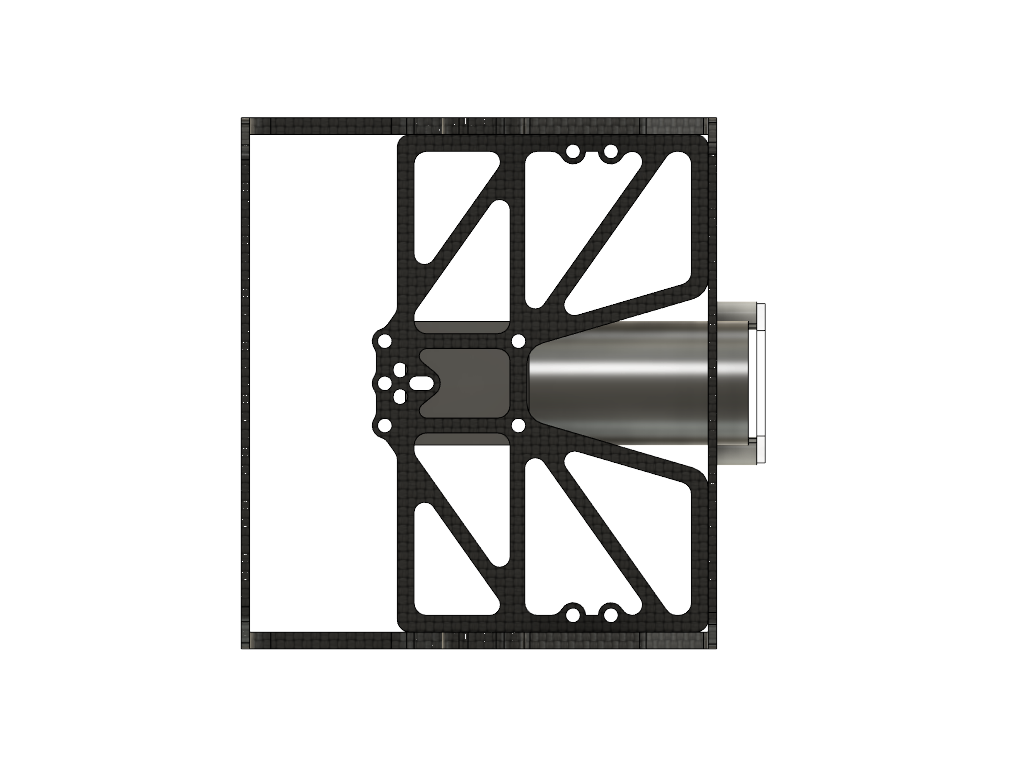
\includegraphics[width=0.6\columnwidth]{figure/设计方案/机械结构设计/大恒相机固定仰视图.png}
        \end{minipage}
    }
    \caption{大恒相机固定展示 \label{fig:大恒相机_设计方案}}
\end{figure} 

如 \figref {fig:电路板_设计方案}
所展示，机器人各个电路模块都是使用螺丝与板件固定，以云台为例，中心板通过四根螺丝固定在底板上，两个电调通过四根螺丝固定在左右两侧板上，且各个板件通过板板连接件互相连接成一个封闭的盒子，以保护盒子中的各个电路模块，避免在比赛中因为受到弹丸的击打而损坏。

\begin{figure}[hbt!]
    \centering
    \subfigure[电路板放置侧视图 \label{fig:电路板1_设计方案} ]{
        \begin{minipage}[t]{0.45\linewidth}
        \centering
        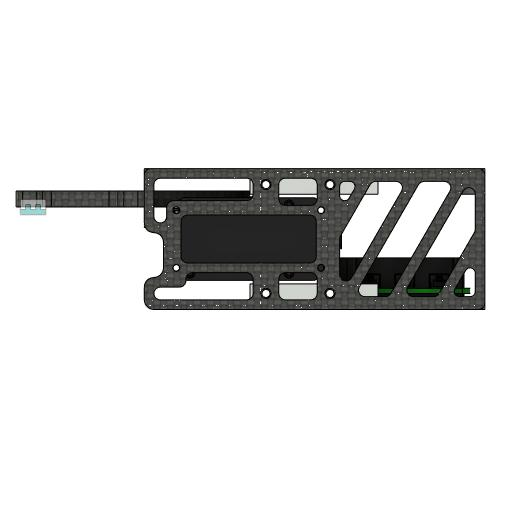
\includegraphics[width=0.6\columnwidth]{figure/设计方案/机械结构设计/电路板放置侧视图.jpg}
        \end{minipage}
    }
    \subfigure[电路板放置俯视图\label{fig:电路板2_设计方案}]{
        \begin{minipage}[t]{0.45\linewidth}
        \centering
        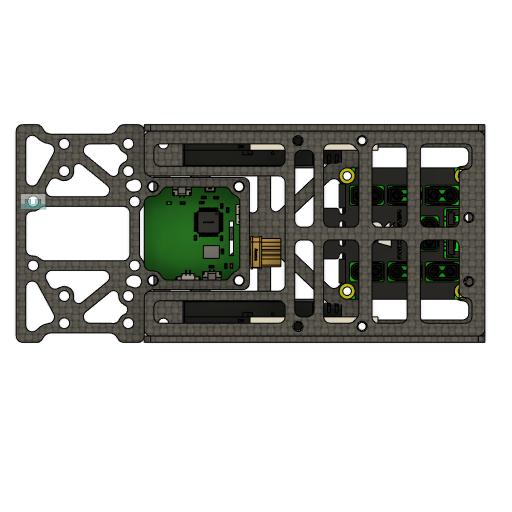
\includegraphics[width=0.6\columnwidth]{figure/设计方案/机械结构设计/电路板放置俯视图.jpg}
        \end{minipage}
    }
    \caption{电路板放置展示 \label{fig:电路板_设计方案}}
\end{figure} 


\subsection{核心零件的有限元分析、静动力学分析}
分析案例为一体式云台安装座，在设定约束条件为$4$个螺栓固定圆柱面，车体处在水平面运动状态下，载荷情况为$\qty{200}{\newton}$单向力（竖直向下）$\qty{1300}{\newton}$单向力（竖直向上）以及$\qty{200}{\newton\meter}$力矩（相当于$\qty{2}{\kilogram}$的重物所提供的负载力在加速度大小为$\qty{10}{\meter\per\s\squared}$的运动状态下）。各种数据是从设想车体受到冲击时，其负载力的竖直分量和力矩。

如 \figref {fig:有限元1_设计方案}
所展示，仿真结果仍然具有15的最低安全系数，考虑实际工况的载荷比仿真载荷要低很多，且当前安全系数显示该零件至少仍可承受15倍当前载荷，可得该零件的强度已经很满足真实应用场景，甚至飞坡时云台Yaw轴与底盘连接处发生断裂的可能性都较小。

如 \figref {fig:有限元2_设计方案}
所展示，在载荷情况与有限元分析一致的情况，且车体处在水平面运动状态下，有限元仿真结果的最大位移量为$\qty{0.001932}{\mm}$，可见其零件刚性也十分满足真实应用场景，正常水平运动不会因为刚性问题导致云台抖动。   

如 \figref {fig:有限元3_设计方案}，如 \figref {fig:有限元4_设计方案}
所展示，安装座底面有螺纹孔固定约束。车体在水平面静止状态下，两侧4个螺丝孔里边下表面有$\qty{20}{\newton}$的垂直向下的单向力。仿真结果的最大应力为$\qty{8.277}{\MPa}$，最大应变基本为$0$，完全符合需求。

\begin{figure}[hbt!]
    \centering 
    \subfigure[安全系数图\label{fig:有限元1_设计方案} ]
        {
        \centering
        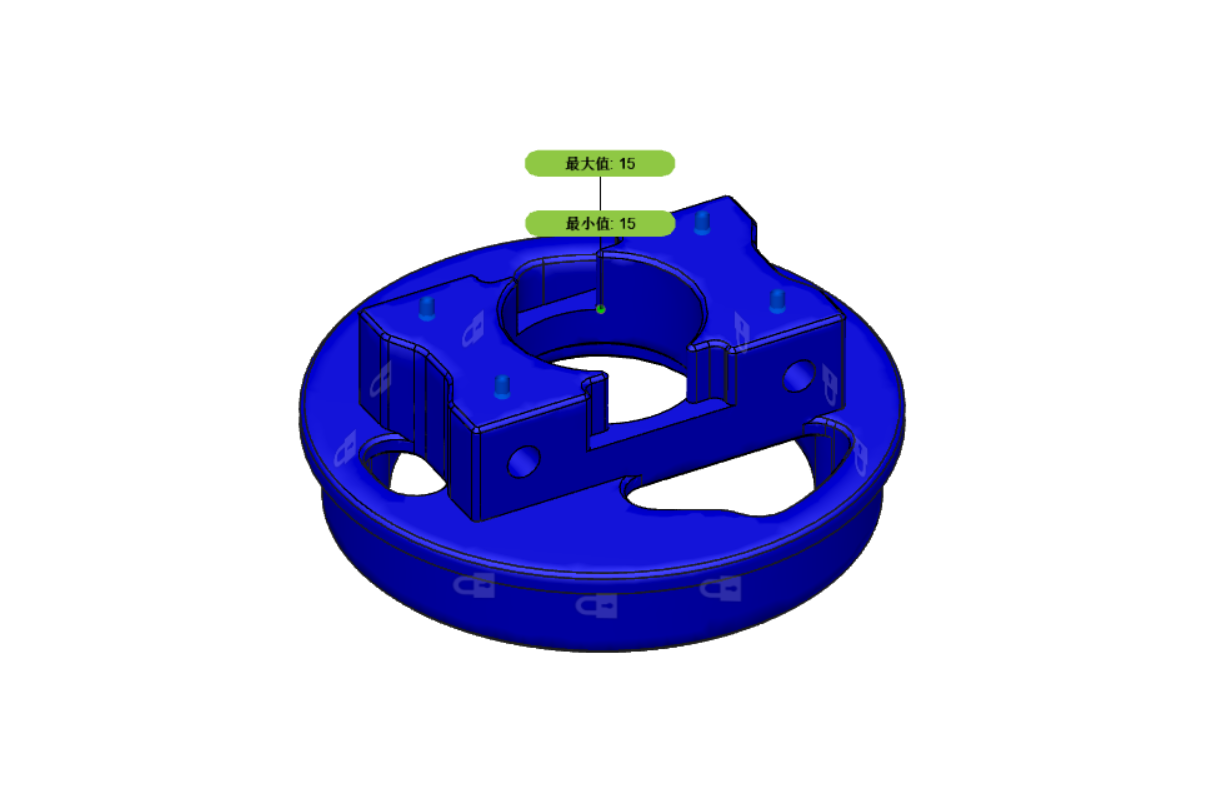
\includegraphics[width=0.35\columnwidth]{figure/设计方案/机械结构设计/安全系数图.png}
        }
    \centering 
    \subfigure[位移图\label{fig:有限元2_设计方案} ]{
        \centering
        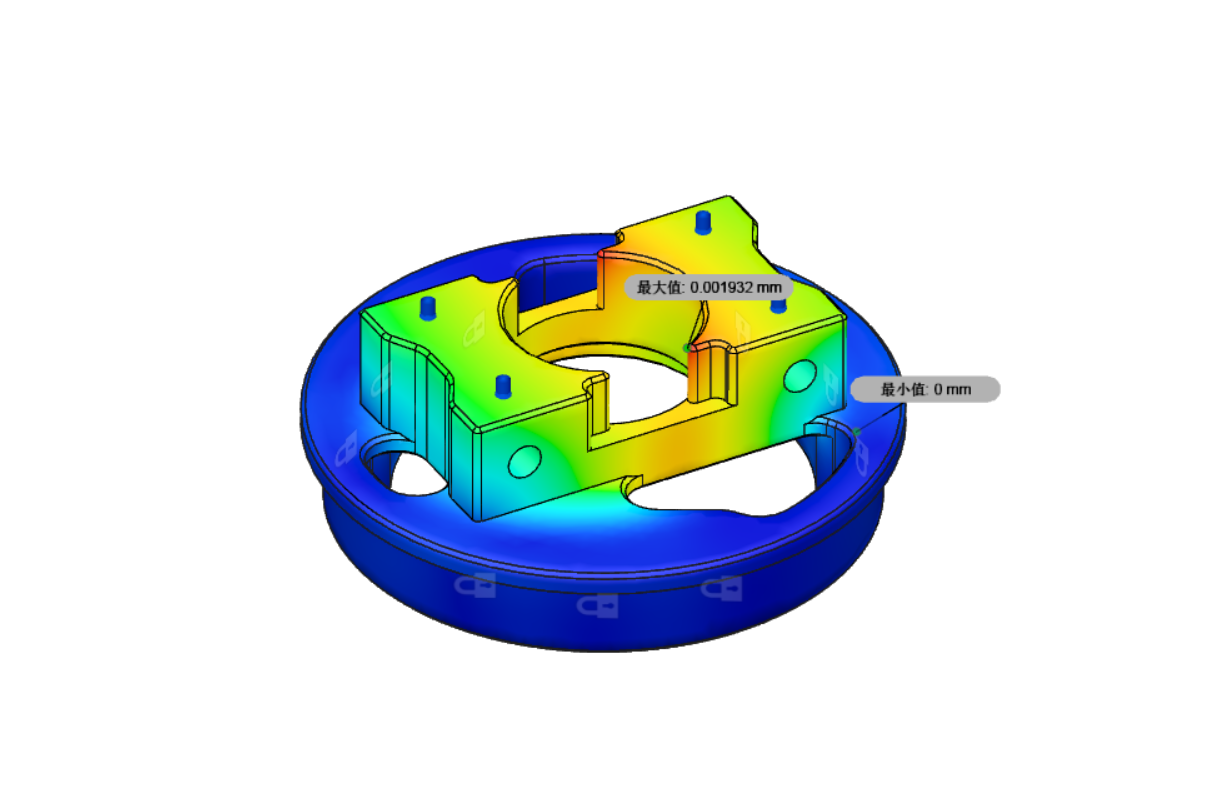
\includegraphics[width=0.35\columnwidth]{figure/设计方案/机械结构设计/位移图.png}
        }    
\end{figure}

\begin{figure}[hbt!]
    \centering 
    \subfigure[应力图\label{fig:有限元3_设计方案} ]{
        \centering
        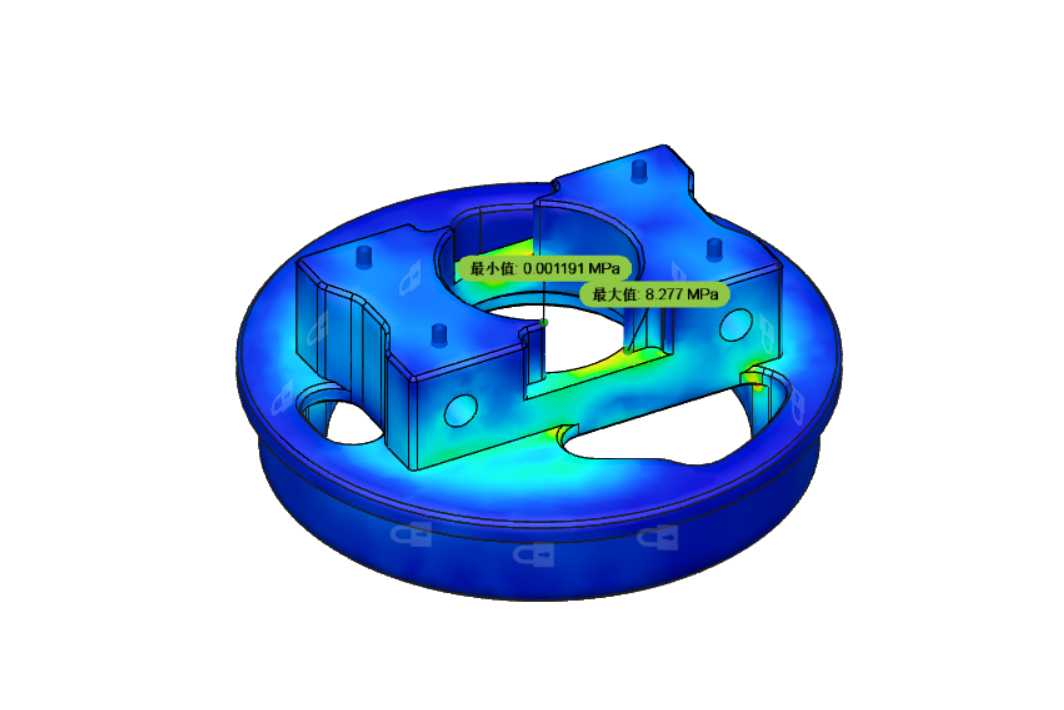
\includegraphics[width=0.35\columnwidth]{figure/设计方案/机械结构设计/应力图.png}
        }
    \subfigure[应变图\label{fig:有限元4_设计方案} ]{
        \centering
        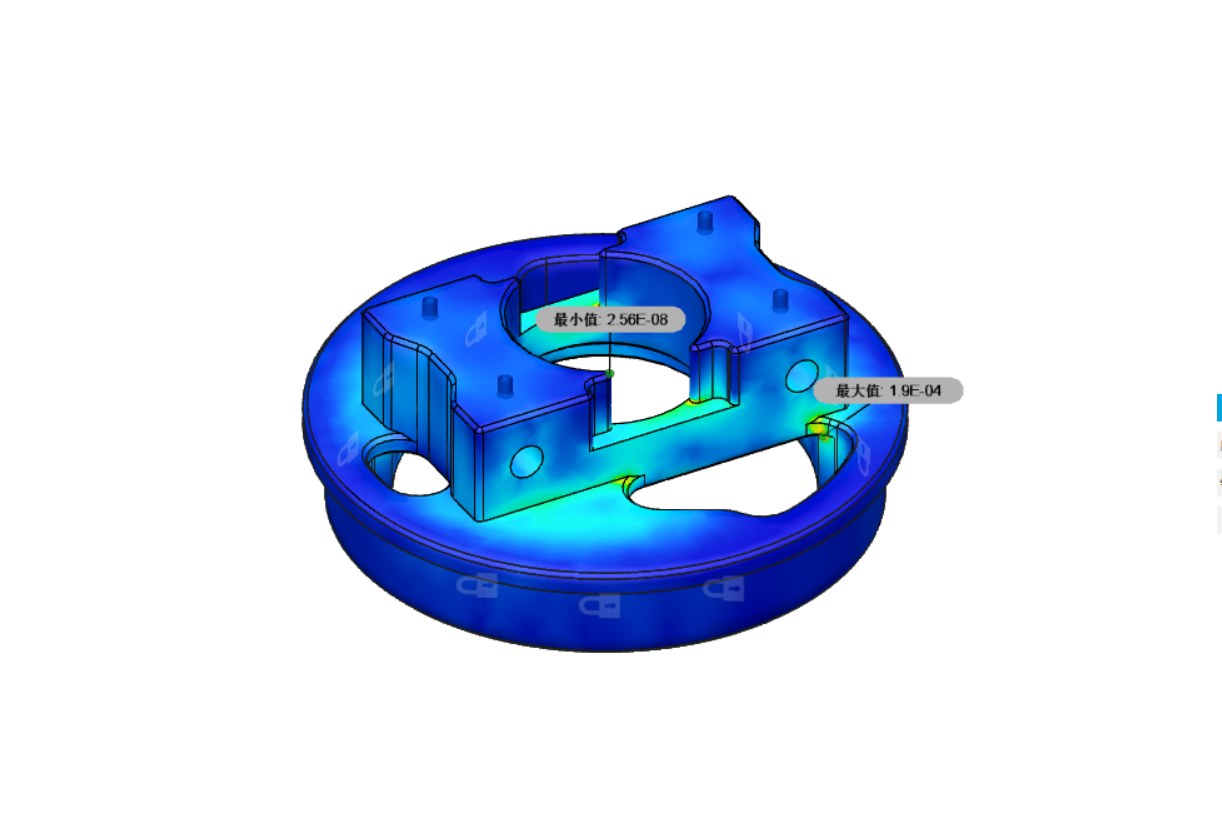
\includegraphics[width=0.35\columnwidth]{figure/设计方案/机械结构设计/应变图.png}
        }
     \caption{有限元仿真分析展示 \label{fig:有限元_设计方案}}
\end{figure} 

\clearpage